\documentclass{config/apuntes}

\title{Fundamentos de Secuenciación de Alto Rendimiento y Genómica Traslacional}
\author{Sandra Mingo Ramírez}
\date{2024/25}
\acronym{HTSTRG}

\usepackage[all]{nowidow}
\usepackage{listing}
\usepackage{color}
\usepackage{tabularx}
\usepackage{multirow}
\usepackage{makecell}
\usepackage{amsmath}
\usepackage{array}
\usepackage{soul}

\definecolor{dkgreen}{rgb}{0,0.6,0}
\definecolor{gray}{rgb}{0.5,0.5,0.5}
\definecolor{mauve}{rgb}{0.58,0,0.82}

\lstset{
  frame=tb,
  aboveskip=3mm,
  belowskip=3mm,
  showstringspaces=false,
  columns=flexible,
  basicstyle={\small\ttfamily},
  numbers=none,
  numberstyle=\tiny\color{gray},
  keywordstyle=\color{blue},
  commentstyle=\color{dkgreen},
  stringstyle=\color{mauve},
  breaklines=true,
  breakatwhitespace=true,
  tabsize=3
}

\usepackage{tocloft}

\advance\cftchapnumwidth 0.5em\relax
\advance\cftsecnumwidth 0.5em\relax
\advance\cftsubsecindent 0.5em\relax
\advance\cftsubsecnumwidth 0.5em\relax
\begin{document}

\begin{abstract}
La asignatura aborda las tecnologías y metodologías actuales para la generación y análisis de datos multi-ómicos en biología y biomedicina, con un enfoque en técnicas de secuenciación masiva (NGS). Se estudian variantes genómicas puntuales y estructurales - como mutaciones, polimorfismos de nucleótido único (SNPs) y variantes en el número de copias génicas (CNVs) - que explican la variabilidad genética poblacional y su relación con enfermedades humanas.

A lo largo del curso, se aplican herramientas bioinformáticas para el análisis de datos reales, profundizando en la epidemiología molecular y los estudios de asociación genómica (GWAS) para explorar los factores de riesgo asociados a variantes genómicas en contextos clínicos y poblacionales. También se revisa el uso de datos genómicos en tratamientos personalizados, considerando su aplicación actual y potencial en la clínica.
\end{abstract}

\pagestyle{plain}

\maketitle

\tableofcontents

%Bloque 1: caracterización del genoma por NGS - introducción a genómica traslacional, métodos de secuenciación, aligners and NGS formats, avances tecnológicos en NGS, NGS for genome assembly, variantes estructurales
%Bloque 2: Genomic variants: techniques, variant calling and annotation - identification of genetic variants, practical exercise, annotation of genetic variants, filtering and prioritization of genetic variants
%Bloque 3: Genome-Wide Association Analysis (GWAS) - technologies, QC, statistical methods, practical exercises
%Bloque 4: Molecular epidemiology - biobanks, mendelian, oligogenic and complex traits, genetic susceptibility and PRS
%Examen tipo test 80% 
%Presentación 20%

%28/10 - Fátima Sánchez Cabo
\part{Caracterización del genoma mediante NGS}
\chapter{Introducción a la genómica traslacional}
\section{Definición e importancia de la genómica}
La genómica, el estudio integral del ADN y de la estructura, función y dinámica de los genomas, representa un pilar fundamental en la biología moderna. Marcó un cambio de paradigma, pasando de un enfoque reduccionista en biología - donde se estudiaban componentes individuales y de manera aislada - a una perspectiva integradora que analiza las interacciones y relaciones entre los distintos elementos biológicos. Esta transición permitió evolucionar de la genética clásica, basada en hipótesis concretas, hacia la genómica, que integra análisis de datos masivos sin necesidad de preguntas iniciales específicas, aunque sí en constante búsqueda de respuestas biológicas complejas.

En el marco del dogma central de la biología, las “ómicas” representan tres niveles de estudio: la genómica (centrada en el ADN), la transcriptómica (ARN) y la proteómica (proteínas). Este curso se enfoca en la genómica, ya que la información genética determina las funciones bioquímicas y, por ende, los fenotipos de los organismos. Gracias a avances recientes, ahora es posible inferir la función bioquímica de las proteínas directamente a partir de la secuencia de ADN, sin necesidad de técnicas complejas como la cristalización. Además, herramientas de inteligencia artificial pueden predecir la estructura de las proteínas con precisión, acelerando la interpretación de funciones biológicas.

Las proteínas, incluyendo enzimas esenciales, son los elementos funcionales clave en la biología. La secuencia de aminoácidos en una cadena polipeptídica define sus propiedades funcionales, y, por tanto, conocer la secuencia genética subyacente (el ADN) facilita predecir la función de una proteína. Aunque determinar experimentalmente las propiedades de una proteína es complejo, la secuenciación genómica ha simplificado enormemente este proceso.

La mejora en tecnologías de secuenciación impulsó el \textbf{Proyecto Genoma Humano}, que logró identificar entre 20,000 y 25,000 genes y determinar la secuencia de los aproximadamente 3 mil millones de pares de bases del genoma humano. Este proyecto también fomentó la creación de bases de datos y herramientas para el análisis de datos genómicos, además de abrir el debate sobre los aspectos éticos, legales y sociales (conocidos como ELSI, por sus siglas en inglés), que siguen siendo temas vigentes y complejos en la actualidad.

\subsection{Evolución de la bioinformática en la genómica}
La bioinformática ha crecido a la par de la genómica en múltiples niveles. Inicialmente, era una \textbf{disciplina} incipiente y se desarrollaba como apoyo experimental; sin embargo, ha evolucionado hasta convertirse en un campo esencial que impulsa la investigación. En cuanto a su \textbf{material, los datos,} la bioinformática ha tenido que adaptarse al fenómeno del big data, pasando de manejar cantidades limitadas de datos a enfrentar volúmenes masivos, propios de la genómica actual. Paralelamente, el \textbf{rol de los bioinformáticos} se transformó, pasando de ser técnicos a científicos de datos y académicos altamente reconocidos en la industria y en la investigación.

\begin{figure}[htbp]
\centering
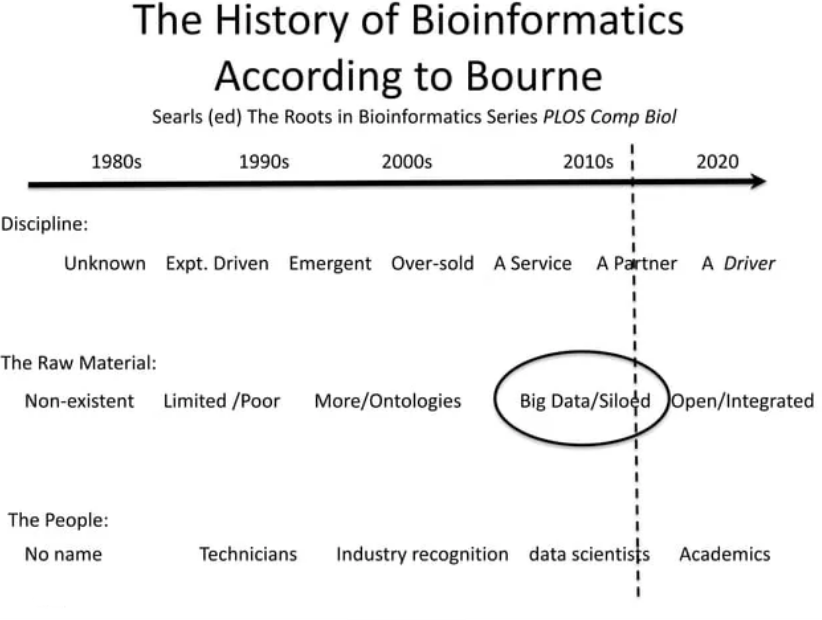
\includegraphics[width = 0.5\textwidth]{figs/history-bioinfo.png}
\caption{Breve historia de la bioinformática en tres niveles: como disciplina, como material que utiliza y como las personas que trabajan en ella. Evolución desde 1980 hasta 2020.}
\end{figure}

\section{Avances tecnológicos en secuenciación}
Existen distintos tipos de tecnologías de secuenciación, comúnmente clasificadas en tres generaciones: la primera generación (first generation), la segunda o Next Generation Sequencing (NGS) y la tercera generación. Las dos primeras generaciones se enfocan en la secuenciación de fragmentos cortos de ADN, mientras que la tercera generación permite la lectura de fragmentos largos, facilitando el ensamblaje completo de genomas. Actualmente, uno de los mayores desafíos tecnológicos es detectar variantes de baja frecuencia y realizar secuenciaciones de ADN en células individuales (single-cell sequencing), lo cual tradicionalmente se hacía de forma masiva (“bulk”).

\begin{figure}[htbp]
\centering
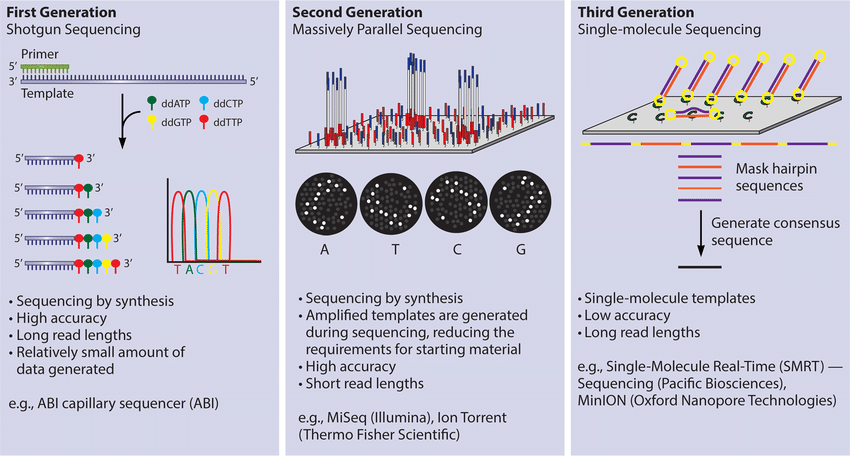
\includegraphics[width = 0.7\textwidth]{figs/sequencing-generations.png}
\caption{Las tres generaciones de secuenciación y su forma de actuar.}
\end{figure}

A medida que el costo de la secuenciación ha disminuido y la capacidad de almacenamiento ha mejorado desde 1990, los datos generados también han crecido exponencialmente. En un experimento de secuenciación, los costos abarcan tanto la secuenciación en sí como el procesamiento bioinformático, el reporte y el almacenamiento de los datos. La comunidad científica y muchos journals requieren que los datos de proyectos financiados públicamente estén disponibles en bases de datos accesibles, lo que asegura la transparencia y el acceso a esta información valiosa. Para obtener una cobertura de calidad, el ADN suele secuenciarse al menos 30 veces, lo que genera archivos de gran tamaño, como los archivos FastQ, que almacenan información de secuencia y calidad para cada base.

\section{Procesos de llamada y priorización de variantes}
Los datos de secuenciación se procesan en pipelines bioinformáticas que comienzan con archivos FastQ normalmente comprimidos y pasan por varias etapas: control de calidad, alineamiento y llamada de variantes (variant calling). Las variantes identificadas pueden incluir cambios de nucleótidos, variaciones en el número de copias de segmentos genómicos (copy number variation) o reordenamientos estructurales.

\begin{figure}[htbp]
\centering
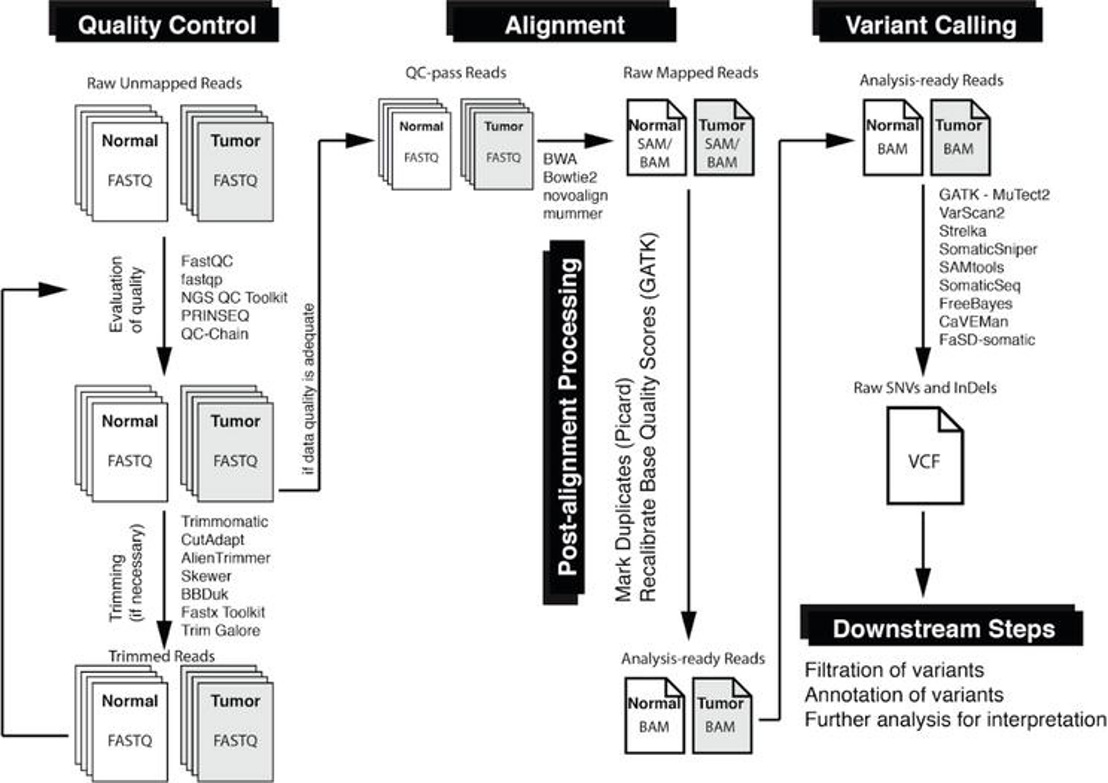
\includegraphics[width = 0.7\textwidth]{figs/bioinfo-pipeline.png}
\caption{Esquema de la pipeline que se sigue en bioinformática para la llamada de variantes.}
\end{figure}

La priorización de variantes se basa en factores como el impacto funcional, la frecuencia alélica en la población y la asociación con enfermedades. Sin embargo, muchas variantes requieren validación experimental, frecuentemente en modelos animales como ratones, para corroborar su relevancia funcional. El proceso de filtrado inicial se enfoca en variantes en exones de genes candidatos, analizando su frecuencia, patogenicidad y modelo de herencia; en caso de no hallarse variantes relevantes, se amplía el análisis a variantes oligogénicas o no codificantes.

\begin{figure}[htbp]
\centering
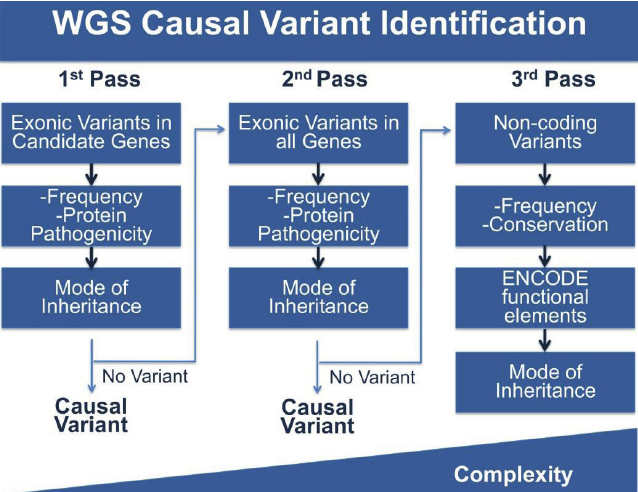
\includegraphics[width = 0.5\textwidth]{figs/variant-priorization.png}
\caption{Ejemplo de la priorización de variantes.}
\end{figure}

\section{Genómica en medicina de precisión}
La genómica ha transformado el enfoque de la medicina de precisión, permitiendo identificar enfermedades con bases genéticas, ambientales o una combinación de ambas. Algunas variantes genéticas confieren una predisposición a enfermedades sin ser causantes directas, lo cual es crucial para inferir relaciones causales y acelerar ensayos clínicos mediante la integración de grandes volúmenes de datos. Estas variantes pueden clasificarse en germinales (heredadas) o somáticas (adquiridas).

\begin{figure}[htbp]
\centering
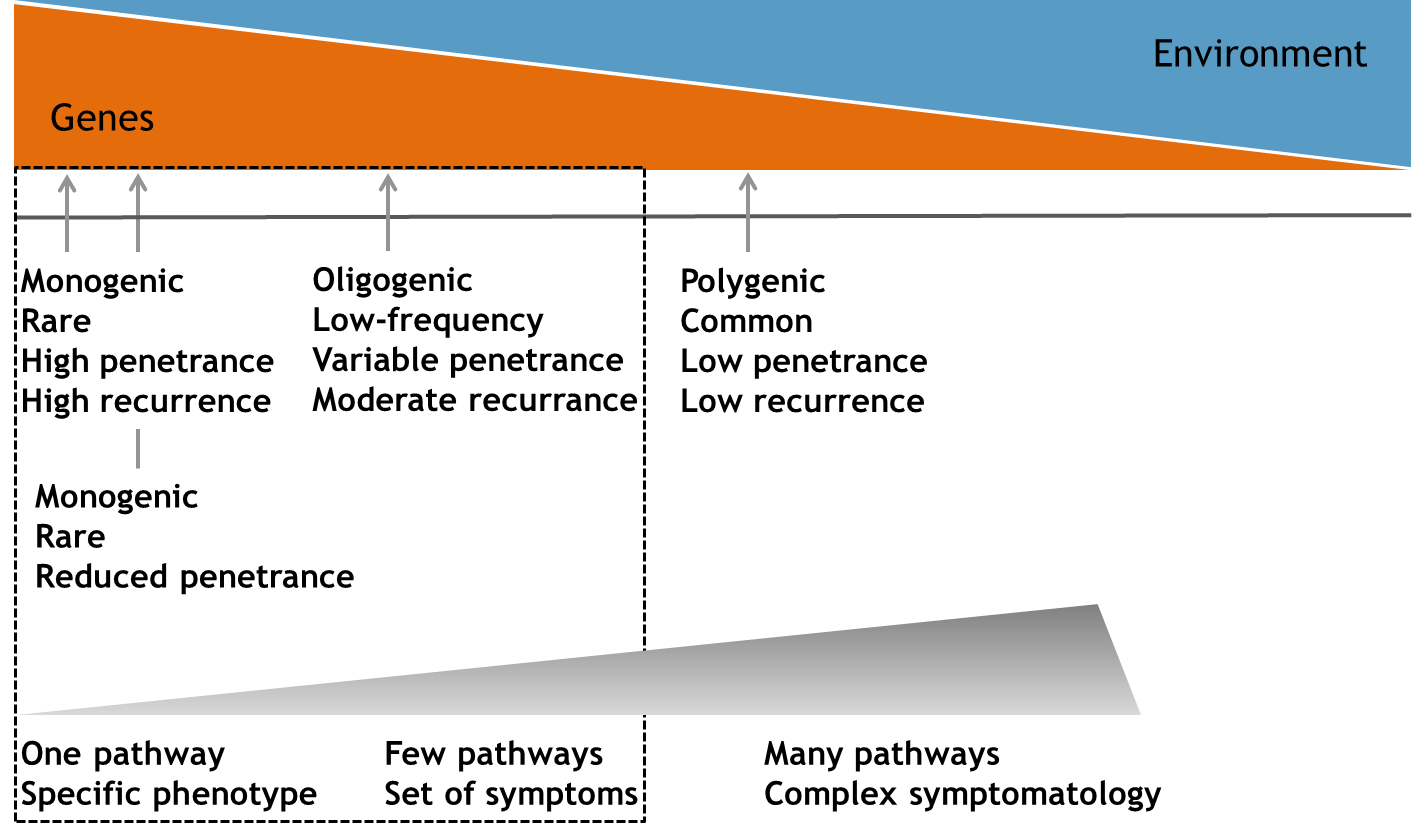
\includegraphics[width = 0.5\textwidth]{figs/genetic-environment.png}
\caption{Representación gráfica de la relación entre enfermedades con base genética, ambientales o una mezcla de ambas.}
\end{figure}

En medicina de precisión, la genómica es solo una capa de datos entre muchas. Para una comprensión holística de la salud y la enfermedad, es necesario combinarla con información de otras “ómicas” como la transcriptómica, epigenómica, proteómica, metabolómica, y datos de microbioma. Además, los datos clínicos y epidemiológicos también forman parte del ecosistema de \textbf{Big Data Biomédico}, que actualmente se maneja mediante técnicas avanzadas de computación en clusters HPC, computación en la nube y algoritmos de GPU.

\begin{figure}[htbp]
\centering
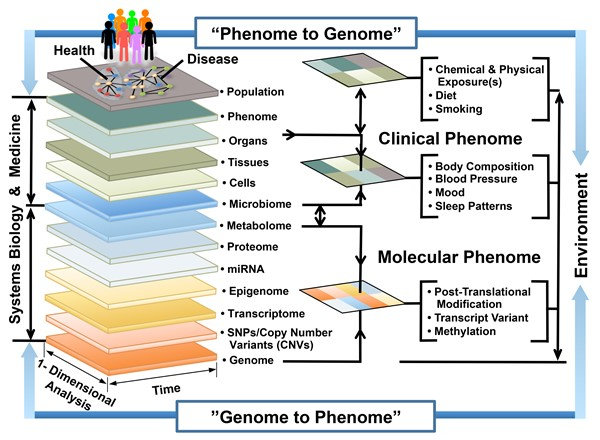
\includegraphics[width = 0.7\textwidth]{figs/bigger-picture-bioinfo.jpg}
\caption{Esquema representando el dibujo general de la bioinformática.}
\end{figure}

Varias bases de datos públicas permiten estudiar la transición entre salud y enfermedad. El estudio de Farmingham, por ejemplo, lleva más de 70 años recolectando datos de factores de riesgo cardiovascular en más de 15,000 participantes. En Reino Unido, el Biobank y, en Estados Unidos, la iniciativa All of Us, también representan recursos de gran envergadura. En España, el CNIC (Centro Nacional de Investigaciones Cardiovasculares) realiza el estudio PESA (Progression of Early Subclinical Atherosclerosis), que ha contribuido a identificar factores predictivos de aterosclerosis subclínica mediante el estudio multiómico, generando nuevos indicadores con un mayor poder predictivo de la formación de placas de colesterol.

\subsection{Epigenética y la medición de la edad biológica}
El perfil de metilación del ADN es un factor epigenético que puede modificar la expresión genética y se ha utilizado para calcular la “edad biológica” o epigenética de una persona, lo que puede servir como predictor de esperanza de vida y salud. Al comparar estos perfiles con la edad cronológica, sexo y otros factores, se obtiene información sobre el envejecimiento y el riesgo de enfermedades, facilitando el desarrollo de estrategias de salud personalizadas.

\section{Resumen}
La genómica ha liderado una revolución científica en el siglo XX, evolucionando desde el estudio de componentes individuales hasta una perspectiva integral de sistemas biológicos y de investigación basada en datos masivos. La bioinformática se ha convertido en una disciplina central en el análisis genómico y predicción de estructuras proteicas, impulsada por el Proyecto Genoma Humano y el desarrollo de tecnologías de secuenciación. Los avances actuales buscan no solo la secuenciación del ADN, sino también la integración de estos datos con datos epidemiológicos y moleculares para obtener una comprensión más profunda de la salud y la enfermedad. Así, el Proyecto Genoma Humano fue decisivo para sentar las bases de tecnologías de secuenciación, el desarrollo de la bioinformática en sí y el uso social e industrial de los datos ómicos.

La identificación de características genómicas relevantes causales de rasgos/enfermedades se basa en la anotación de variantes en bases de datos y en estudios poblacionales: hay margen de mejora y un gran éxito de la ciencia colaborativa. Hoy en día, los principales proyectos tratan no sólo de secuenciar el ADN, sino de integrar esta información con datos epidemiológicos y otros datos moleculares para comprender mejor la salud y la enfermedad.
Las enfermedades, en función de su base genética, pueden clasificarse en monogénicas (mendelianas), oligogénicas (ej., cardiopatías familiares) y complejas (evaluadas mediante puntuaciones de riesgo poligénicas). Esta clasificación permite avanzar en la medicina de precisión, abordando enfermedades desde su origen genético para ofrecer intervenciones de salud más efectivas y personalizadas.

%30/10 - Álvaro Serrano
\chapter{Métodos de secuenciación}
La secuenciación permite pasar de la información contenida en el ADN a un dominio digital mediante una representación abstracta. 

El primer método de secuenciación fue el \textbf{método Maxam-Gilbert} (figura \ref{fig:MaxamGilbert}), que utilizaba un marcador en el extremo 5' del ADN. En este proceso, el ADN se trataba con diferentes compuestos químicos para provocar rupturas específicas en función de cada base nitrogenada. Los fragmentos resultantes se separaban en un gel de acrilamida mediante electroforesis, y se revelaban mediante autoradiografía de rayos X. La secuencia se deducía observando el patrón de bandas resultante. Para los curiosos \href{https://www.youtube.com/watch?v=_B5Dj8PL4E0}{véase ésto}.

\begin{figure}[htbp]
\centering
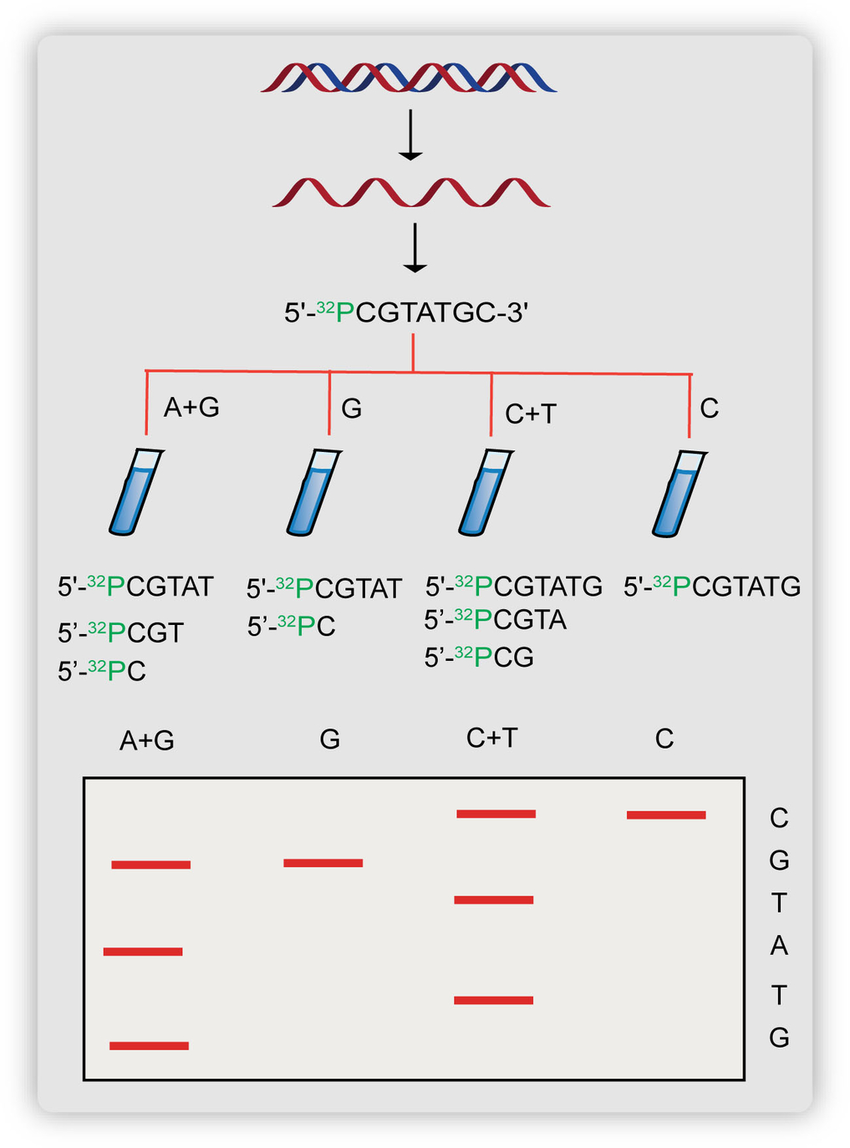
\includegraphics[width = 0.3\textwidth]{figs/maxam-gilbert.png}
\caption{\textbf{Principio de la secuenciación Maxam-Gilbert}: Las copias del fragmento de ADN monocatenario que se desea secuenciar se marcan radioactivamente y se les somete a cuatro reacciones de degradación de bases por separado (A+G, G, C+T y C). Se obtienen fragmentos de ADN de diferente longitud tras la escisión del resto de la cadena en las zonas degradadas. Los productos se cargan en cuatro pocillos separados de un gel de poliacrilamida. La secuencia se lee de abajo a arriba como GTATGC. Si se encuentra una G frente a un hueco en el gel, se confirma que se trata de 5-metilcitosina en la cadena molde.}
\label{fig:MaxamGilbert}
\end{figure}

Otro método clave es el de \textbf{terminación de cadena, o método de Sanger} (figura \ref{fig:Sanger}). Este utiliza deoxinucleótidos modificados, que tienen un átomo de hidrógeno en el grupo 2' de la pentosa, en lugar de un grupo hidroxilo (OH). Esto impide la unión del extremo 5' al 3', deteniendo así la extensión de la cadena de ADN. El resultado es una mezcla de fragmentos de distintos tamaños, los cuales se marcan con isótopos radioactivos o, en versiones más modernas, con fluoróforos. La secuencia se obtiene mediante detección de colores en una única reacción, simplificando el análisis. La clave de este método \marginpar[\footnotesize Pregunta examen] \ es el uso de dideoxinucleótidos, que interrumpen la actividad de la ADN polimerasa, permitiendo detener la cadena de manera controlada.

\begin{figure}[htbp]
\centering
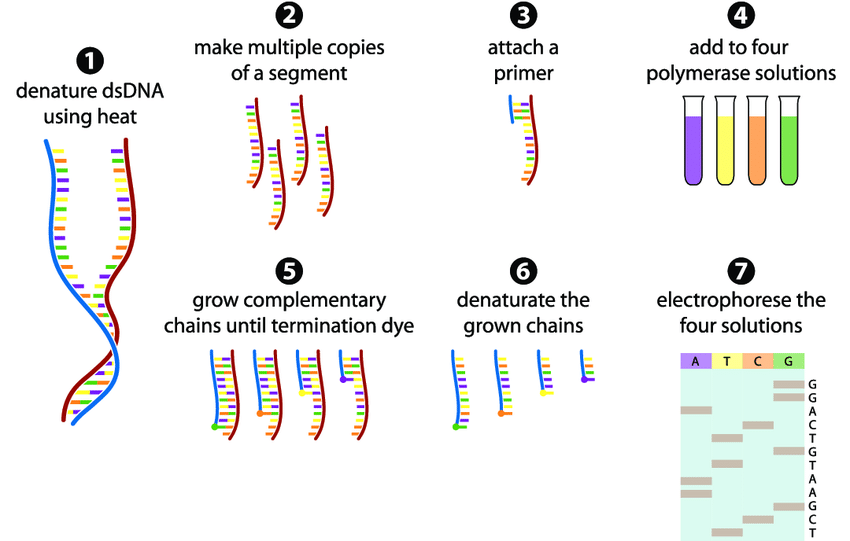
\includegraphics[width = 0.8\textwidth]{figs/sanger.png}
\caption{\textbf{El método de secuenciación Sanger en 7 pasos.} (1) El fragmento de dsADN se desnaturaliza en dos fragmentos de ssADN. (2) Un fragmento de ssADN se multiplica en millones de copias. (3) Se une un cebador que corresponde a un extremo del fragmento. (4) Los fragmentos se añaden a cuatro soluciones de polimerasa. Cada solución contiene los cuatro tipos de bases pero sólo un tipo de nucleótido de terminación. (5) La cadena crece hasta que se añade aleatoriamente un nucleótido de terminación. (6) Los fragmentos de dsADN resultantes se desnaturalizan para obtener una serie de ssADN de distintas longitudes. (7) Los fragmentos se separan por electroforesis y se lee la secuencia.}
\label{fig:Sanger}
\end{figure}

El primer secuenciador automático fue el ABI370, capaz de secuenciar hasta 5000 bases al día. Sin embargo, se necesitarían aproximadamente 16,000 años para secuenciar todo el genoma humano usando esta tecnología. Este secuenciador innovador reemplazaba los geles por electroforesis capilar y un detector de fluorescencia. Durante el Proyecto Genoma Humano en los años 90 y 2000, desarrollado en colaboración entre el sector público y privado, se introdujeron mejoras significativas a los secuenciadores, como el modelo ABI377, que empleaba varios capilares para incrementar la eficiencia. Sin embargo, la secuenciación de regiones altamente repetitivas del genoma, como los telómeros y centrómeros, fue compleja, y la primera descripción completa del genoma humano fue publicada hace apenas un año.

\section{Shotgun genome sequencing y Proyecto Genoma Humano}
A finales de los 90, comenzó el PGH. Los métodos que se utilizaron en el proyecto fueron \href{https://www.youtube.com/watch?v=aShY577MoM0}{los siguientes} (figura \ref{fig:PGH}):
\begin{itemize}
\item \textbf{Hierarchical Shotgun:} Fue el primer método en utilizarse. La idea era fragmentar el genoma humano en fragmentos grandes (150-350kb) en BACs. Entonces, a partir de estos genomas bacterianos el ADN se clona (plásmidos) en fragmentos más pequeños (2-10kb) usando enzimas de restricción. Y se volvían a fragmentar (usando distintas ER) para secuenciarse. Finalmente, se buscaban los solapamientos entre secuencias para formar contigs, los cuales se ensamblan progresivamente para reconstruir la secuencia original. 
\item \textbf{Whole-genome Shotgun:} Similar al método anterior, pero se realiza directamente sobre el genoma completo en lugar de partir de cromosomas bacterianos. El ADN se clona en bacterias, se fragmenta y se ensamblan los contigs mediante solapamiento.
\end{itemize}

\begin{figure}[htbp]
\centering
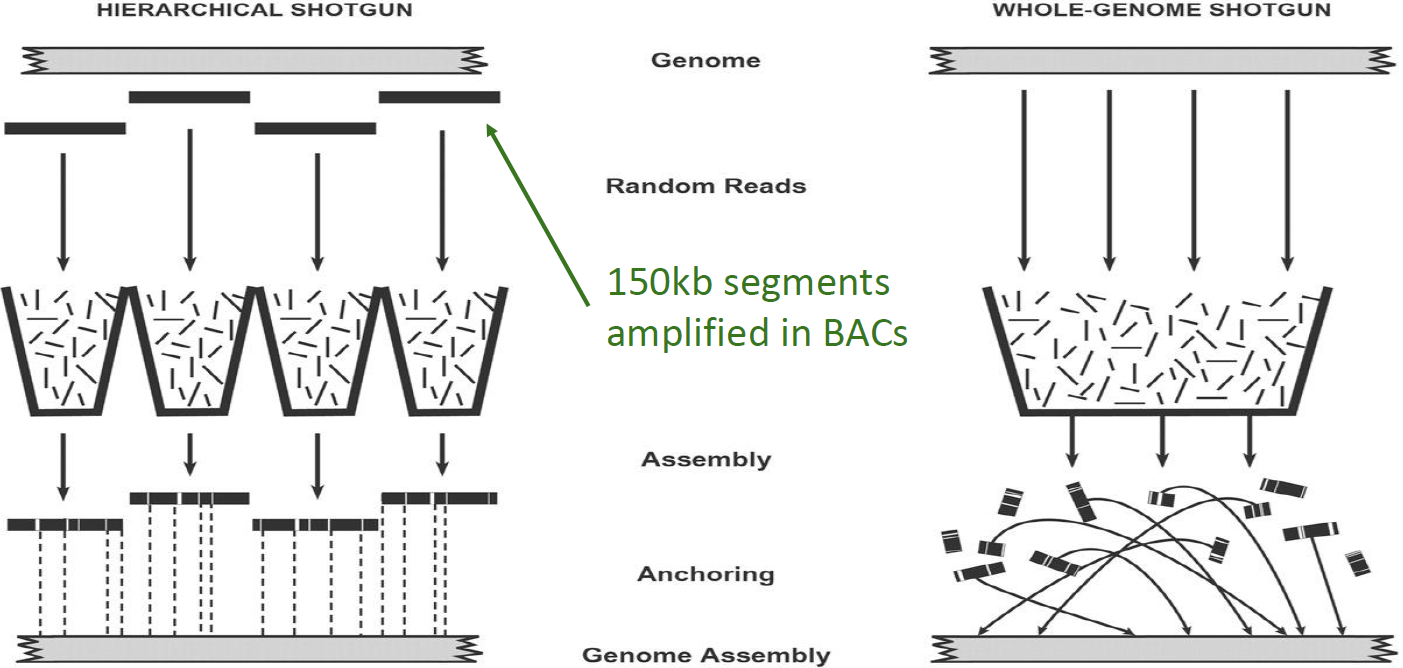
\includegraphics[width = 0.8\textwidth]{figs/HGP-sequencing.png}
\caption{\textbf{Estrategias de secuenciación en el Proyecto Genoma Humano.} (Izquierda) La estrategia de hierarchical shotgun (HS) consiste en descomponer el genoma en un camino de mosaico de clones BAC (bacterial artificial chromosome) superpuestos, realizar la secuenciación en cada BAC y volver a ensamblarlo, y luego fusionar las secuencias de clones adyacentes. El método tiene la ventaja de que todos los contigs de secuencias y scaffolds derivados de un BAC pertenecen a un único compartimento con respecto al anclaje al genoma. (Derecha) La estrategia WGS (Whole-genome shotgun) consiste en secuenciar todo el genoma e intentar reensamblar toda la colección. Con el método WGS, cada contig y scaffold es un componente independiente que debe anclarse al genoma. En general, muchos scaffolds no pueden anclarse sin esfuerzos dirigidos. (Los contigs son bloques contiguos de secuencia; los scaffolds son conjuntos de contigs unidos por lecturas emparejadas de ambos extremos de un inserto plasmídico).}
\label{fig:PGH}
\end{figure}

La electroforesis capilar, usada en ambos métodos, permite separar fragmentos de ADN de diferentes tamaños a través de un capilar con un detector de fluorescencia, logrando una lectura precisa de aproximadamente 500 pares de bases por fragmento. Con el tiempo, los costos de secuenciación disminuyeron gracias a avances en técnicas posteriores al método de Sanger.

\section{NGS: la siguiente generación de tecnología de secuenciación del ADN}
La secuenciación de segunda generación o Next-Generation Sequencing (NGS) permite una secuenciación paralela y masiva, también conocida como \textbf{high-throughput sequencing}. Los principales métodos NGS incluyen 454 Roche, Solexa Illumina, ABI/SOLiD, Complete Genomics, Pacific Biosciences, Ion Torrent y Oxford Nanopore. Estas tecnologías amplifican los fragmentos de la molécula de ADN original. 

\subsection{Preparación de librerías de NGS}
Las librerías de secuenciación se preparan fragmentando el ADN y generando secuencias que luego se amplifican y procesan en el secuenciador, obteniendo las lecturas o reads. Estas librerías se amplifican clonalmente mediante tres métodos:
\begin{itemize}
\item \textbf{Beads:} pequeñas bolitas recubiertas de primers, donde el ADN se adhiere y se amplifica.
\item \textbf{Fase sólida:} el ADN se adhiere a una superficie de cristal donde se amplifica.
\item \textbf{Nanobolas:} se produce un ovillo de ADN amplificado en forma circular, que se adhiere a una placa metálica funcionalizada (con grupos funcionales) para secuenciación.
\end{itemize}

La secuenciación NGS utiliza un gran número de moléculas idénticas, permitiendo una secuenciación paralela de alta eficiencia y alto rendimiento o high-throughput. La característica de la segunda generación es que utiliza la molécula de ADN original y, sobre ella, la amplifica, es decir, la utiliza como molde para generar muchas moléculas iguales. 

\subsection{Clasificación de NGS: secuenciación por síntesis y por ligación}
Los métodos de secuenciación de segunda generación se pueden clasificar en secuenciación por síntesis (con la enzima polimerasa) o secuenciación por ligación (con la enzima ligasa).

\begin{itemize}
\item \textbf{Secuenciación por síntesis (SBS)}
\begin{itemize}
\item \textbf{Ciclo de terminación reversible (CRT) Illumina/Solexa:} una evolución del método Sanger. Se utiliza ADN unido a beads o cristales y se añaden dNTPs modificados con el grupo 3’ OH bloqueado, limitando así la acción de la polimerasa y parando la duplicación de la cadena. Cada ciclo implica la incorporación de un nucleótido, seguido de una señal fluorescente específica del nucleótido unido. Posteriormente, el grupo OH se desbloquea con un químico de lavado para que el proceso continúe. La señal que se detecta no es de un único nucleótido, si no del conjunto de nucleótidos del cluster, que debido a la amplificación clonal, debería ser la misma señal amplificada. Esto se realiza por el límite de detección de fluorescencia de los microscopios. Además, la placa con los moldes tiene en los límites unos marcadores que permiten que el microscopio se enfoque a la altura a la que debe. Se ve representado en la figura \ref{fig:CRT}.

\begin{figure}[htbp]
\centering
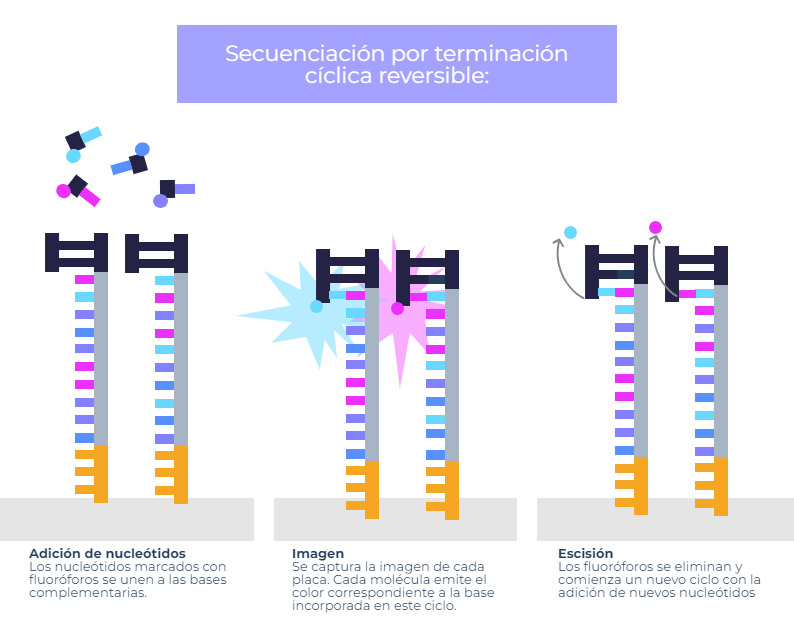
\includegraphics[width = 0.7\textwidth]{figs/secuenciacion-terminacion-ciclica-reversible.jpg}
\caption{\textbf{Secuenciación por terminación cíclica reversible:}
Esta metodología se basa en la utilización de nucleótidos marcados con fluoróforos en una reacción de síntesis de ADN. Cada vez que uno de estos nucleótidos se incorpora a la cadena, el sistema toma una captura y registra de qué tipo de nucleótido se trata. Una vez tomada la captura, se eliminan los fluoróforos de los nucleótidos que se han incorporado y se continúa la síntesis de la cadena con nuevos nucleótidos marcados.}
\label{fig:CRT}
\end{figure}

Una vez terminada la secuenciación, se utiliza como primer para secuenciar la cadena contraria. Esto se debe a que el microscopio va enfocando peor y se pierde calidad. Cada señal emitida por el fluoróforo se conoce como call o llamada. Cada call tiene una confident score de Q, que se calcula mediante la fórmula $Q = - 10 \cdot log_{10} P $. Por tanto, si Q es 30, P sería $10^{-3}$, representando P la probabilidad de error. La información que se obtiene en el archivo es la secuencia obtenida con un valor Q asociado codificado en ASCII. 

Los microscopios se clasifican en microscopios de 4 canales y de 2 canales (figura \ref{fig:microscope-channel}). Los microscopios de 4 canales tienen una mayor calidad al poder distinguir cada uno de los nucleótidos, mientras que los de 2 canales utilizan la combinación de dos fluoróforos: se detecta verde, rojo, la combinación entre verde y rojo, y la ausencia de fluorescencia. Esto último es algo arriesgado, ya que algunos nucleótidos podrían perder el fluoróforo y se consideraría ausencia de fluorescencia. No obstante, estos microscopios de 2 canales, pese a tener una peor calidad, son más rápidos y baratos. Respecto al secuenciador, hay varios tipos, por lo que al elegir uno se tendrá que tener cuenta el caso de uso y el dinero disponible (la página de Illumina tiene tablas comparativas para elegir el mejor secuenciador para cada caso). 

\begin{figure}[htbp]
\centering
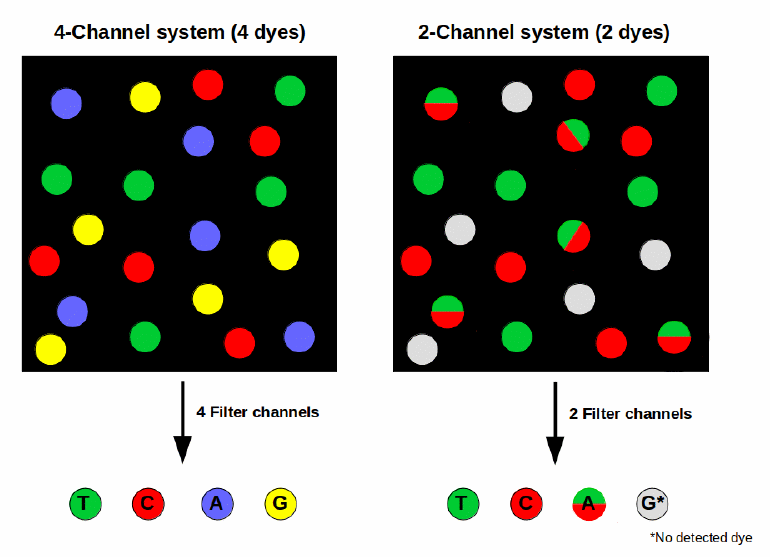
\includegraphics[width = 0.7\textwidth]{figs/microscope-channels.png}
\caption{Comparación entre los microscopios de 4 y de 2 canales.}
\label{fig:microscope-channel}
\end{figure}

Las ventajas de la secuenciación CRT es que es la que produce la mayor cantidad de secuencias secuenciadas a la vez (mayor throughput), con mayor precisión y longitud de lectura de las NGS (estándar actual con 2 canales). La desventaja es el límite que puede secuenciar, que es en torno a 150 bases por cada extremo. 

\item \textbf{Adición de nucleótidos simple (SNA):} en cada ciclo se añade un solo tipo de nucleótido, detectando su incorporación. Este método es sensible a los homopolímeros (repeticiones del mismo nucleótido), pero puede generar problemas de fase si la señal no es proporcional al número de nucleótidos añadidos. Por lo que puede tener problemas con los homopolímeros muy largos.
\begin{itemize}
\item \textbf{Pirosecuenciación:} emplea pirofosfato liberado en la síntesis de ADN. Debido a su enlace de alta energía, la acción de la pirofosfatasa acoplada a la luciferasa produce que se emita una señal de luz proporcional al número de nucleótidos añadidos. Este método es rápido, económico y preciso, aunque presenta limitaciones con secuencias largas debido al cambio de fase en el momento en el que se produzca un error. La calidad de la secuenciación es Q45 (99,997\%). Se ve representado en la figura \ref{fig:pirosecuenciacion}.

\begin{figure}[htbp]
\centering
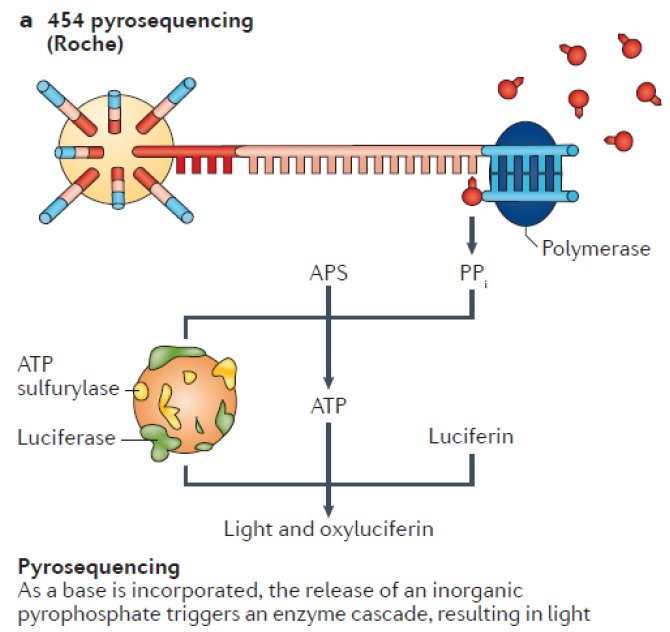
\includegraphics[width = 0.5\textwidth]{figs/pirosecuenciacion.png}
\caption{Esquema de la pirosecuenciación, tecnología que permite determinar el orden de una secuencia de ADN mediante luminiscencia.}
\label{fig:pirosecuenciacion}
\end{figure}

\item \textbf{Ion Torrent proton detection:} mide el cambio de pH (cambio de potencial) que ocurre al liberar un protón durante la polimerización del ADN. Al final de cada ciclo es necesario lavar para evitar la señal cruzada. La técnica es económica y ampliamente utilizada en hospitales, pero presenta desafíos con secuencias largas debido a la falta de proporcionalidad en la señal en secuencias con regiones muy repetitivas (si se unen dos nucleótidos en lugar de uno, la señal es proporcional a los dos, pero cuando se unen 50 nucleótidos, el cambio de potencial no es proporcional a los 50). Se ve representado en la figura \ref{fig:iontorrent}.

\begin{figure}[htbp]
\centering
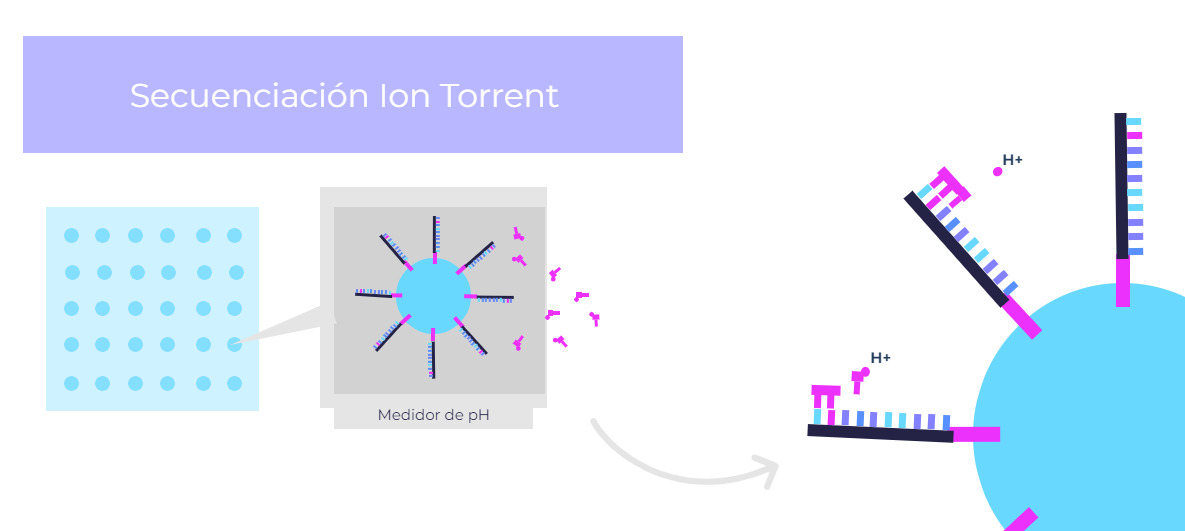
\includegraphics[width = 0.7\textwidth]{figs/Ion-torrent-sequencing.jpg}
\caption{\textbf{Secuenciación por Ion Conductor (Ion Torrent Sequencing):} 
Se trata de una estrategia que se basa en la detección de las modificaciones en el pH que se producen en la síntesis de ADN. Para ello, se van incorporando nucleótidos a una cadena de ADN, provocando que se libere un protón (H+) en la reacción y, por tanto, que se vea modificado el pH. Para poder diferenciar cuál de los cuatro tipos de nucleótidos se ha introducido en cada posición de la secuencia, se repiten varios ciclos, cada uno de ellos, con la adición de un único tipo de nucleótido. }
\label{fig:iontorrent}
\end{figure}

\end{itemize}
\end{itemize}

\item \textbf{Secuenciación por ligación (SBL)}
\begin{itemize}
\item \textbf{Secuenciación por SOLiD:} Este método (poco utilizado) emplea sondas de ligación con dos bases complementarias a la base que se secuencia. En cada ciclo, una ligasa une una sonda marcada con un fluoróforo y luego se elimina la fluorescencia para repetir el ciclo, generando datos precisos, aunque menos comunes en la práctica. Se van mapeando dos nucleótidos a la vez, dejando un espacio de 3 nucleótidos. Por ello, se repite cinco veces añadiendo espaciadores (offsets) que corren el sitio de unión de la sonda y permitan el solapamiento de las lecturas. Figura \ref{fig:solid}.

\begin{figure}[htbp]
\centering
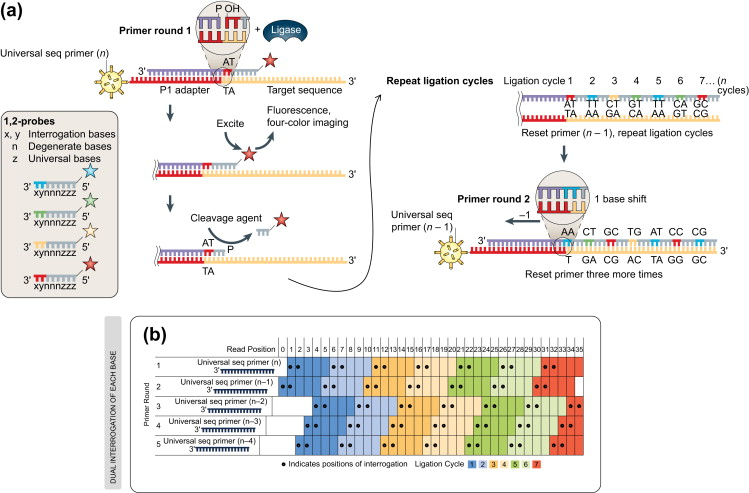
\includegraphics[width = \textwidth]{figs/solid-sequencing.jpg}
\caption{\textbf{Ilustración del método de secuenciación por ligación utilizando la plataforma SOLiD.} (a) Esquema de los diferentes pasos seguidos por el método SOLiD de ligadura por cuatricromía: hibridación de primers, ligadura selectiva de las sondas, obtención de imágenes por cuatricromía y escisión de la sonda. El ciclo SOLiD se repite nueve veces más. El producto de extensión se elimina y la plantilla se reajusta con un cebador complementario a la posición n -1 para una segunda ronda de ciclos de ligación. (b) Se realizan cinco rondas de reajuste del cebador para cada etiqueta de secuencia. Mediante el procedimiento de reajuste de cebadores, prácticamente todas las bases se consultan en dos reacciones de ligación independientes con dos cebadores diferentes.}
\label{fig:solid}
\end{figure}

\item \textbf{Complete Genomics (Nanoballs, BGI):} El ADN se amplifica mediante rolling circle para formar moléculas de ADN grandes con forma de ovillo (nanobolas o NDB), que luego se hibridan en una placa (la flowcell). El ADN se secuencia de forma iterativa con sondas fluorescentes que se unen por ligacion (como en el método anterior). Este método permite una alta densidad de nanobolas en cada flowcell, teniendo así una precisión muy alta (más que los métodos de SBS). No obstante, ya que sólo permite secuenciar lecturas pequeñas, se utilizan distintos adaptadores a los que se unen las sondas, lo que permite aumentar el throughput. Hay partes de la tecnología que no se conocen y está principalmente disponible en China.
\end{itemize}
\end{itemize}

\subsection{Limitaciones y desafíos en NGS}
La NGS de segunda generación presenta una tasa de error de Q25-Q35 y ciertas limitaciones:
\begin{itemize}
\item \textbf{Lecturas cortas} generan dificultades en el ensamblaje de genomas completos y en la identificación de variantes estructurales.
\item \textbf{Errores de secuenciación} especialmente en regiones complejas y repetitivas, como secuencias AT/GC (SBS) y homopolímeros (SNA).
\item \textbf{Sesgo de amplificación} algunas regiones se amplifican mejor que otras, lo que afecta a la uniformidad en las lecturas.
\item \textbf{Alto coste de los equipos}
\item \textbf{Fenómeno de la cadena retrasada} cuando no se incorpora un nucleótido, produciendo un descabalgamiento del ciclo de lectura real y el ciclo de lectura en el que creemos que estamos.
\item \textbf{Persistencia de errores en los cluster} al producirse un error en el cluster, el error se queda a lo largo de la secuenciación. P.ej.: en el primer ciclo.
\item \textbf{Cambios epigenéticos} pueden afectar negativamente a la precisión de secuenciación por sus diferencias químicas, ya que podría incorcorarse otro nt durante la polimerización. 
\end{itemize}

\section{Resumen}
La secuenciación ha cambiado la forma de hacer y entender la biología. La secuenciación de segunda generación o NGS permite secuenciar millones de moldes de ADN al mismo tiempo. Generalmente, el molde de ADN es amplificado clonalmente, y las llamadas se hacen mediante el consenso de los moldes clonales. Hay dos tipos de secuenciación NGS: por síntesis con la polimerasa o por ligación (SOLiD y Nanoballs). Hay dos tipos de secuenciación por síntesis. La adición simple de nucleótidos (pirosecuenciación 454 y Ion Torrent) añade un dNTP distinto en cada ciclo, pero tiene problemas con moldes homopoliméricos. La terminación cíclica reversible (Illumina) añade todos los dNTP en cada ciclo y secuencia la misma posición en el molde, pero puede sufrir de desfase (con los microscopios de 2 canales).
%Importante a quedar claro: diferencia entre secuenciación por síntesis y por ligación, y dentro de ellos la diferencia entre el método CRT y SNA. Los métodos de ligación hay que saber que existen, pero no es habitual trabajar con ellos. 

\section{Quizz}
\begin{enumerate}
\item Which of the following NGS platforms offers the highest accuracy?
\begin{itemize}
\item Ion Torrent
\item 454
\item Illumina
\item SOLiD
\end{itemize}

Answer: Illumina

\item What is the reversible chain termination method (CRT)?
\begin{itemize}
\item A method that uses modified nucleotides to stop DNA synthesis
\item A method that involves the use of anchors and fluorescent probes
\item A sequencing process based on detecting pH changes
\item A real-time PCR technique
\end{itemize}

Answer: A method that uses modified nucleotides to stop DNA synthesis

\item Which sequencing method employs PCR amplification and ddNTP?
\begin{itemize}
\item Maxam-Gilbert
\item Ion Torrent
\item Sanger
\item Nanoballs
\end{itemize}

Answer: Sanger

\item What is a common problem in second generation sequencing methods?
\begin{itemize}
\item Low cycling efficiency
\item Difficulty detecting homopolymers
\item Low precision in GC regions
\item Very long execution times
\end{itemize}

Answer: Difficulty detecting homopolymers

\item What NGS technology allows real-time sequencing?
\begin{itemize}
\item 454
\item SOLiD
\item Illumina
\item PacBio
\end{itemize}

Answer: PacBio

\item What achievement was reached with the Human Genome Project (HGP)?
\begin{itemize}
\item Sequencing of the complete human genome
\item Sequencing of the mouse genome
\item The first automated sequencing
\item Creation of the nanoball sequencing method
\end{itemize}

Answer: Sequencing of the complete human genome

\item What technology uses circle displacement amplification to generate nanoballs?
\begin{itemize}
\item PacBio
\item SOLiD
\item Illumina
\item BGI
\end{itemize}

Answer: BGI

\item What was the first NGS instrument developed?
\begin{itemize}
\item Illumina
\item Ion Torrent
\item 454
\item SOLiD
\end{itemize}

Answer: 454

\item What error is common in sequencing based on the nucleotide addition method (SNA)?
\begin{itemize}
\item Errors from long reads
\item Errors in low complexity regions
\item Difficulty detecting single nucleotide polymorphisms (SNPs)
\item Problems with homopolymers
\end{itemize}

Answer: Problems with homopolymers

\item What is the basis of the Maxam-Gilbert method for DNA sequencing?
\begin{itemize}
\item Amplification of fragments on a solid surface
\item Use of chemicals to break the DNA molecule
\item Adding nucleotides iteratively
\item Electronic detection of pH changes
\end{itemize}

Answer: Use of chemicals to break the DNA molecule

\item What is one of the main advantages of massively parallel sequencing?
\begin{itemize}
\item Generation of long and accurate reads
\item Ability to sequence multiple DNA templates at the same time
\item Capability to perform sequencing at low cost
\item Reduction of error rates in reads
\end{itemize}

Answer: Ability to sequence multiple DNA templates at the same time

\item What technique uses clonal amplification of DNA on solid surfaces?
\begin{itemize}
\item Ion Torrent
\item Pyrosequencing
\item Sequencing by synthesis
\item Nanoballs
\end{itemize}

Answer: Sequencing by synthesis

\item Which sequencing platform is based on proton detection
\begin{itemize}
\item SOLiD
\item Illumina
\item Ion Torrent
\item PacBio
\end{itemize}

Answer: Ion Torrent

\item What was the main technique used in the Human Genome Project?
\begin{itemize}
\item Maxam-Gilbert
\item Pyrosequencing
\item Sanger sequencing
\item Second generation NGS
\end{itemize}

Answer: Sanger sequencing

\item Which NGS platform is known for its low cost per Mb sequenced?
\begin{itemize}
\item Illumina
\item SOLiD
\item 454
\item Ion Torrent
\end{itemize}

Answer: Ion Torrent

\item What is one of the advantages of reversible terminator sequencing technology (CTR)?
\begin{itemize}
\item Does not require clonal amplification
\item Long read length
\item High accuracy in called bases
\item Can handle RNA templates
\end{itemize}

Answer: High accuracy in called bases

\item What NGS technology uses a system of up to two colors for detection?
\begin{itemize}
\item Ion Torrent
\item Illumina
\item PacBio
\item SOLiD
\end{itemize}

Answer: Illumina

\item What are the disadvantages of second generation sequencing systems?
\begin{itemize}
\item Low precision in SNP detection
\item Short read lengths
\item High costs per sequence
\item Low coverage of repetitive regions
\end{itemize}

Answer: Short read lengths

\item What is the main limitation of pyrosequencing?
\begin{itemize}
\item High error rate in low complexity regions
\item Problems with homopolymers
\item High error rate in short segments
\item Difficulty in detecting structural variants
\end{itemize}

Answer: Problems with homopolymers

\item What is one of the main disadvantages of the SOLiD platform?
\begin{itemize}
\item Problems with long reads
\item High error rate in homopolymers
\item Low precision in variation detection
\item Requires an additional cycle for each read
\end{itemize}

Answer: High error rate in homopolymers

\item Which NGS platform is based on luminescence detection?
\begin{itemize}
\item 454
\item Illumina
\item SOLiD
\item Ion Torrent
\end{itemize}

Answer: 454

\item What is a main disadvantage of second-generation sequencing systems?
\begin{itemize}
\item Low precision in SNP detection
\item Short read lengths
\item High costs per sequence
\item Low coverage of repetitive regions
\end{itemize}

Answer: Short read lengths

\item What key feature defines the Sanger chain termination method?
\begin{itemize}
\item Use of specific enzymes to emit light
\item Use of ddNTPs to stop DNA replication
\item Probe and anchor-based sequencing
\item Use of a microchip with electronic sensors
\end{itemize}

Answer: Use of ddNTPs to stop DNA replication

\item What type of methods are grouped under the term NGS?
\begin{itemize}
\item Massively parallel high-capacity sequencing methods
\item Manual low-precision sequencing methods
\item Methods based on RNA synthesis
\item Methods for detecting three-dimensional structures
\end{itemize}

Answer: Massively parallel high-capacity sequencing methods

\item Which sequencing technique was the first to implement the concept of sequencing by synthesis?
\begin{itemize}
\item Nanoballs
\item SOLiD
\item Sanger
\item 454
\end{itemize}

Answer: Sanger
\end{enumerate}

%04/11 - Álvaro Serrano
\chapter{Alineadores y fomatos de NGS}
\section{Preparación de librería}
Una librería es una colección de fragmentos de ADN de tamaño aleatorio obtenidos a partir de una muestra que se desea secuenciar. El proceso comienza con la extracción del material genético (ADN o ARN -> ADNc), seguido de su fragmentación en piezas pequeñas que posteriormente serán leídas. Los extremos de los fragmentos deben repararse a continuación y se les añade adaptadores (primers conocidos), que permiten su hibridación con una fase sólida donde realizar la amplificación. Finalmente, se purifican los fragmentos para obtener solo las moléculas del tamaño deseado, dependiendo del método de secuenciación que se vaya a utilizar. Por ejemplo, si quisiesemos secuenciar single-end con Illumina, añadir fragmentos de más de 150bp produciría ruido en la secuenciación.

\subsection{Fragmentación del material genético}
Existen distintas aproximaciones en la fragmentación del ADN:
% Mejor empezar por tagmentación porque todo lo que va a continuación va a colación con el de ligación, tanto la rotura, como la reparación, métodos y comparación, etc.
\begin{itemize}
\item \textbf{Aproximación por tagmentación: }
En este método (figura \ref{fig:tagmentacion}), se utiliza la enzima tagmentasa, una transposasa que corta la secuencia de ADN e incorpora adaptadores de manera enzimática \footnote{Los transposones son elementos móviles dentro del ADN.}. La tagmentación es rápida y eficiente, pues combina la fragmentación y la adición de adaptadores en un solo paso.

\begin{figure}[htbp]
\centering
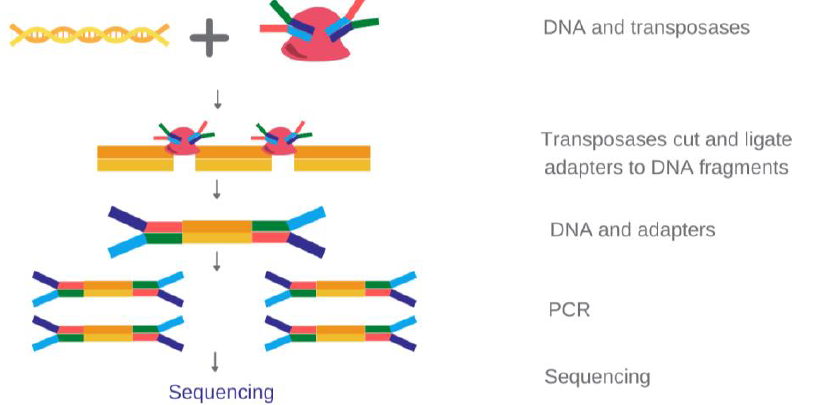
\includegraphics[width = 0.8\textwidth]{figs/tagmentation.png}
\caption{Representación esquemática de la fragmentación por tagmentación.}
\label{fig:tagmentacion}
\end{figure}

\item \textbf{Aproximación por ligación:} 
En este método, la cadena de ADN se puede romper con distintas técnicas (cada una con sus ventajas y desventajas). Los fragmentos de ADN resultantes se reparan añadiendo una adenina en los extremos, lo que permite la unión complementaria de los adaptadores. Esto produce fragmentos con un adaptador en cada extremo. Cada fragmento tiene así dos componentes: la secuencia del adaptador para la secuenciación y la secuencia molde de ADN. Además, cada fragmento puede llevar un identificador único (UMI, por sus siglas en inglés). Los UMIs permiten rastrear la molécula original de la que provienen sus copias y diferenciar los productos con distinta molécula original como, por ejemplo, los de las copias de un gen de dos cromosomas homólogos.

\begin{figure}[htbp]
\centering
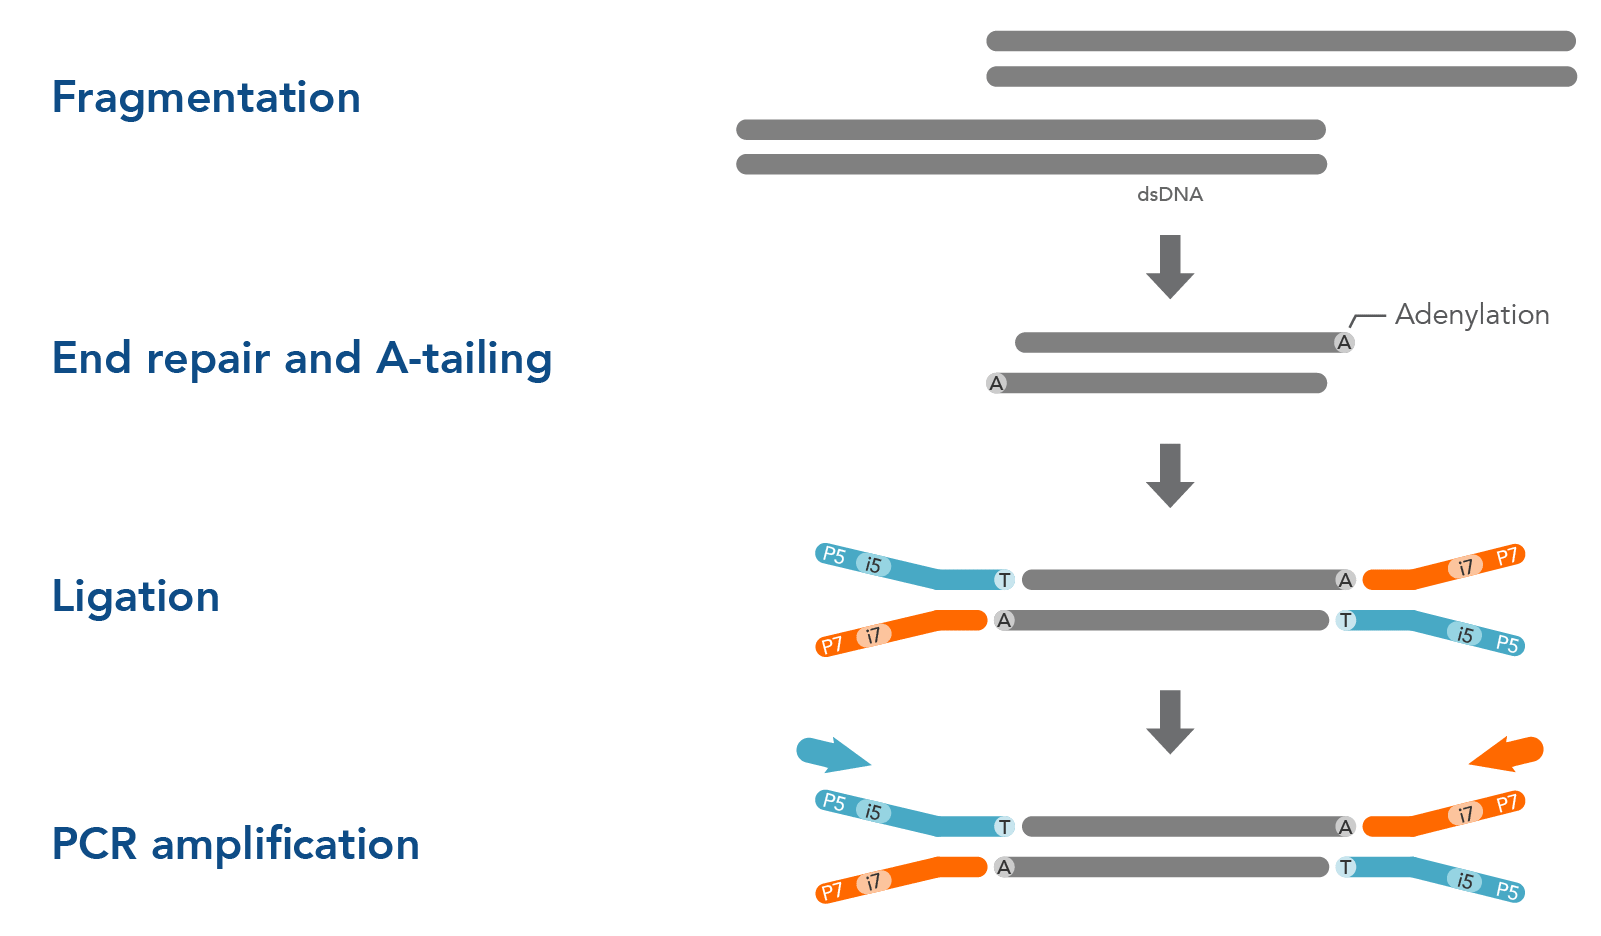
\includegraphics[width = 0.8\textwidth]{figs/19_ng_lib-prep-frag.png}
\caption{Esquema de la preparación de librerías por fragmentación.}
\end{figure}

Las técnicas de fragmentación por ligación (figura \ref{fragmentacion}) incluyen:
\begin{itemize}
\item \textit{Fragmentación física (sonicación)}:
Mediante un sonicador, se aplican ondas sonoras que generan vibración por resonancia, dividiendo el ADN en fragmentos. La frecuencia de las ondas determina el tamaño de los fragmentos obtenidos.
\item \textit{Fragmentación química:}
Se utilizan agentes químicos, como ácidos o bases fuertes, para romper los enlaces fosfodiéster del ADN. Este método es muy barato, pero los químicos fuertes pueden modificar las marcas epigenéticas mediante procesos de oxidación o reducción. Es útil en casos donde la epigenética no es relevante.
\item \textit{Fragmentación enzimática:}
Se emplean endonucleasas, que son enzimas capaces de cortar las cadenas de ADN en puntos específicos, produciendo fragmentos con extremos cohesivos o romos. Es muy barato y fácilmente escalable. Este método permite una fragmentación precisa (cortes en patrón), pero puede introducir sesgos en la representatividad de la librería generada (pérdida de material) si la diana de restricción en cuestión está sub- o sobrerrepresentada en algunas regiones del genoma. Recuérdese el paso de purificación (selección por tamaño de fragmento). Por ello, se suele utilizar un cóctel de ER para evitar soscabar la reprentabilidad de los cortes. 
\end{itemize}

\begin{figure}[htbp]
\centering
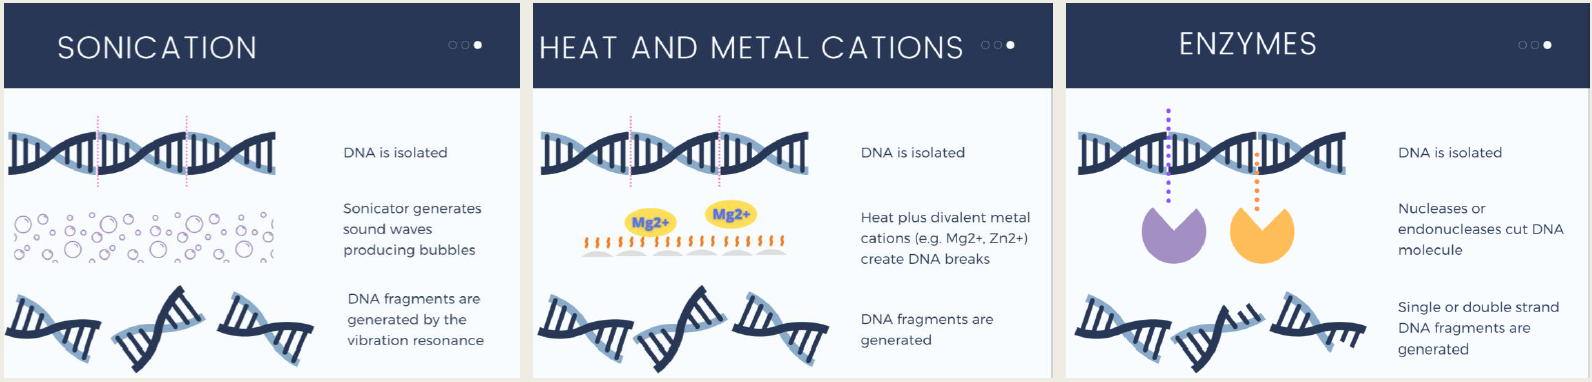
\includegraphics[width = \textwidth]{figs/ligation-methods.png}
\caption{Representación gráfica de los distintos métodos de fragmentación por ligación.}
\label{fragmentacion}
\end{figure}

\begin{table}[htbp]
\centering
\resizebox{\textwidth}{!}{\begin{tabular}{l | l l l}
& Physical & Chemical & Enzymatic \\ \hline \hline
Pro & Broad range & Well for RNA & Standard lab equipment \\
& Unbiased & & Highly scalable \\
& Less sample variation & Lower input of material \\
& Even sized of fragments & & \\
& No interferences & & \\
& Easy to implement & & \\ \hline
Cons & Expensive equipment & Cations interfere with some seq methods & Fragmentation bias \\
& Loss of material (efecto Bach: fragmentos pequeños degradables) & & Ratio material/enzymes \\
& Modification of bases & & Sample-to-sample variation
\end{tabular}}
\caption{Pros y contras de cada método de fragmentación por ligación}
\end{table}
\end{itemize}

\subsection{Reparación de extremos y ligación de adaptadores}
Después de la fragmentación del ADN, es necesario reparar los extremos de los fragmentos. Como la fragmentación no suele producir cortes limpios, los fragmentos generados suelen presentar extremos sobresalientes (overhangs). Para corregir esto, se realiza un tratamiento enzimático con polimerasas, que además añade una adenina (A) en los extremos 3’. Estos extremos, con la adenina añadida, facilitan la ligación de los adaptadores, los cuales suelen tener un overhang de timina (T) para permitir una unión complementaria con los fragmentos de ADN.

\begin{figure}[htbp]
\centering
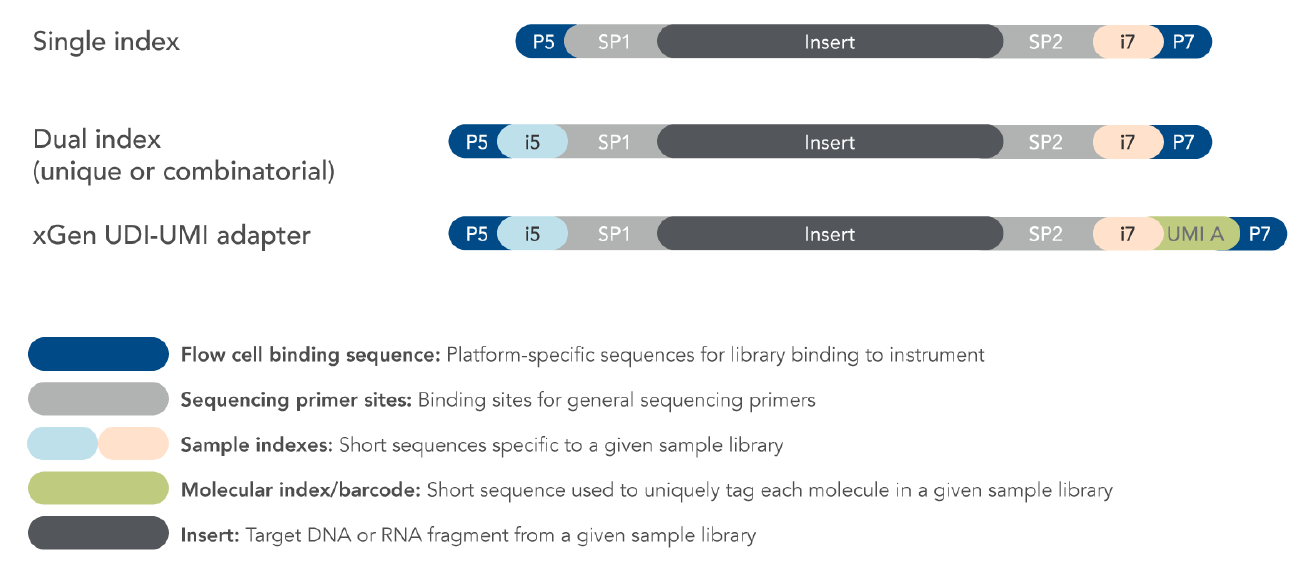
\includegraphics[width = \textwidth]{figs/adaptator.png}
\caption{Representación de los adaptadores en caso de secuenciación simple, dual y UDI-UMI.}
\label{fig:umi}
\end{figure}

Los adaptadores empleados en la secuenciación tienen distintas configuraciones (figura \ref{fig:umi}). Por lo general, se colocan dos tipos de adaptadores:el adaptador P5 (para single-end) en un extremo y el adaptador P7 (se añade para pair-end) en el otro. Esta disposición permite identificar e inducir las direcciones de lectura durante el proceso de secuenciación; dadas las interacciones iónicas y químicas de los adaptadores, se pegan de un lado o de otro. 
Además, algunos adaptadores incluyen identificadores moleculares únicos, conocidos como UMIs (Unique Molecular Identifiers), que permiten rastrear de forma única cada molécula de ADN. Durante la amplificación, todas las moléculas con el mismo UMI corresponden a la misma molécula de ADN original. Esto tiene múltiples beneficios:
\begin{itemize}
\item \textbf{Eliminación de duplicados de PCR:} Permite distinguir duplicados generados por PCR de secuencias originales.
\item \textbf{Disminuir el ratio de error:} La lectura de la misma molécula varias veces permite detectar posibles errores generados durante la construcción de la librería o la amplificación. Si diferentes secuencias presentan un UMI idéntico pero difieren en algún nucleótido, se deduce que ha habido un error, ya que las secuencias deberían ser idénticas. Esto ayuda a reducir el índice de error y a detectar variantes poco frecuentes.
\end{itemize}

\begin{figure}[htbp]
\centering
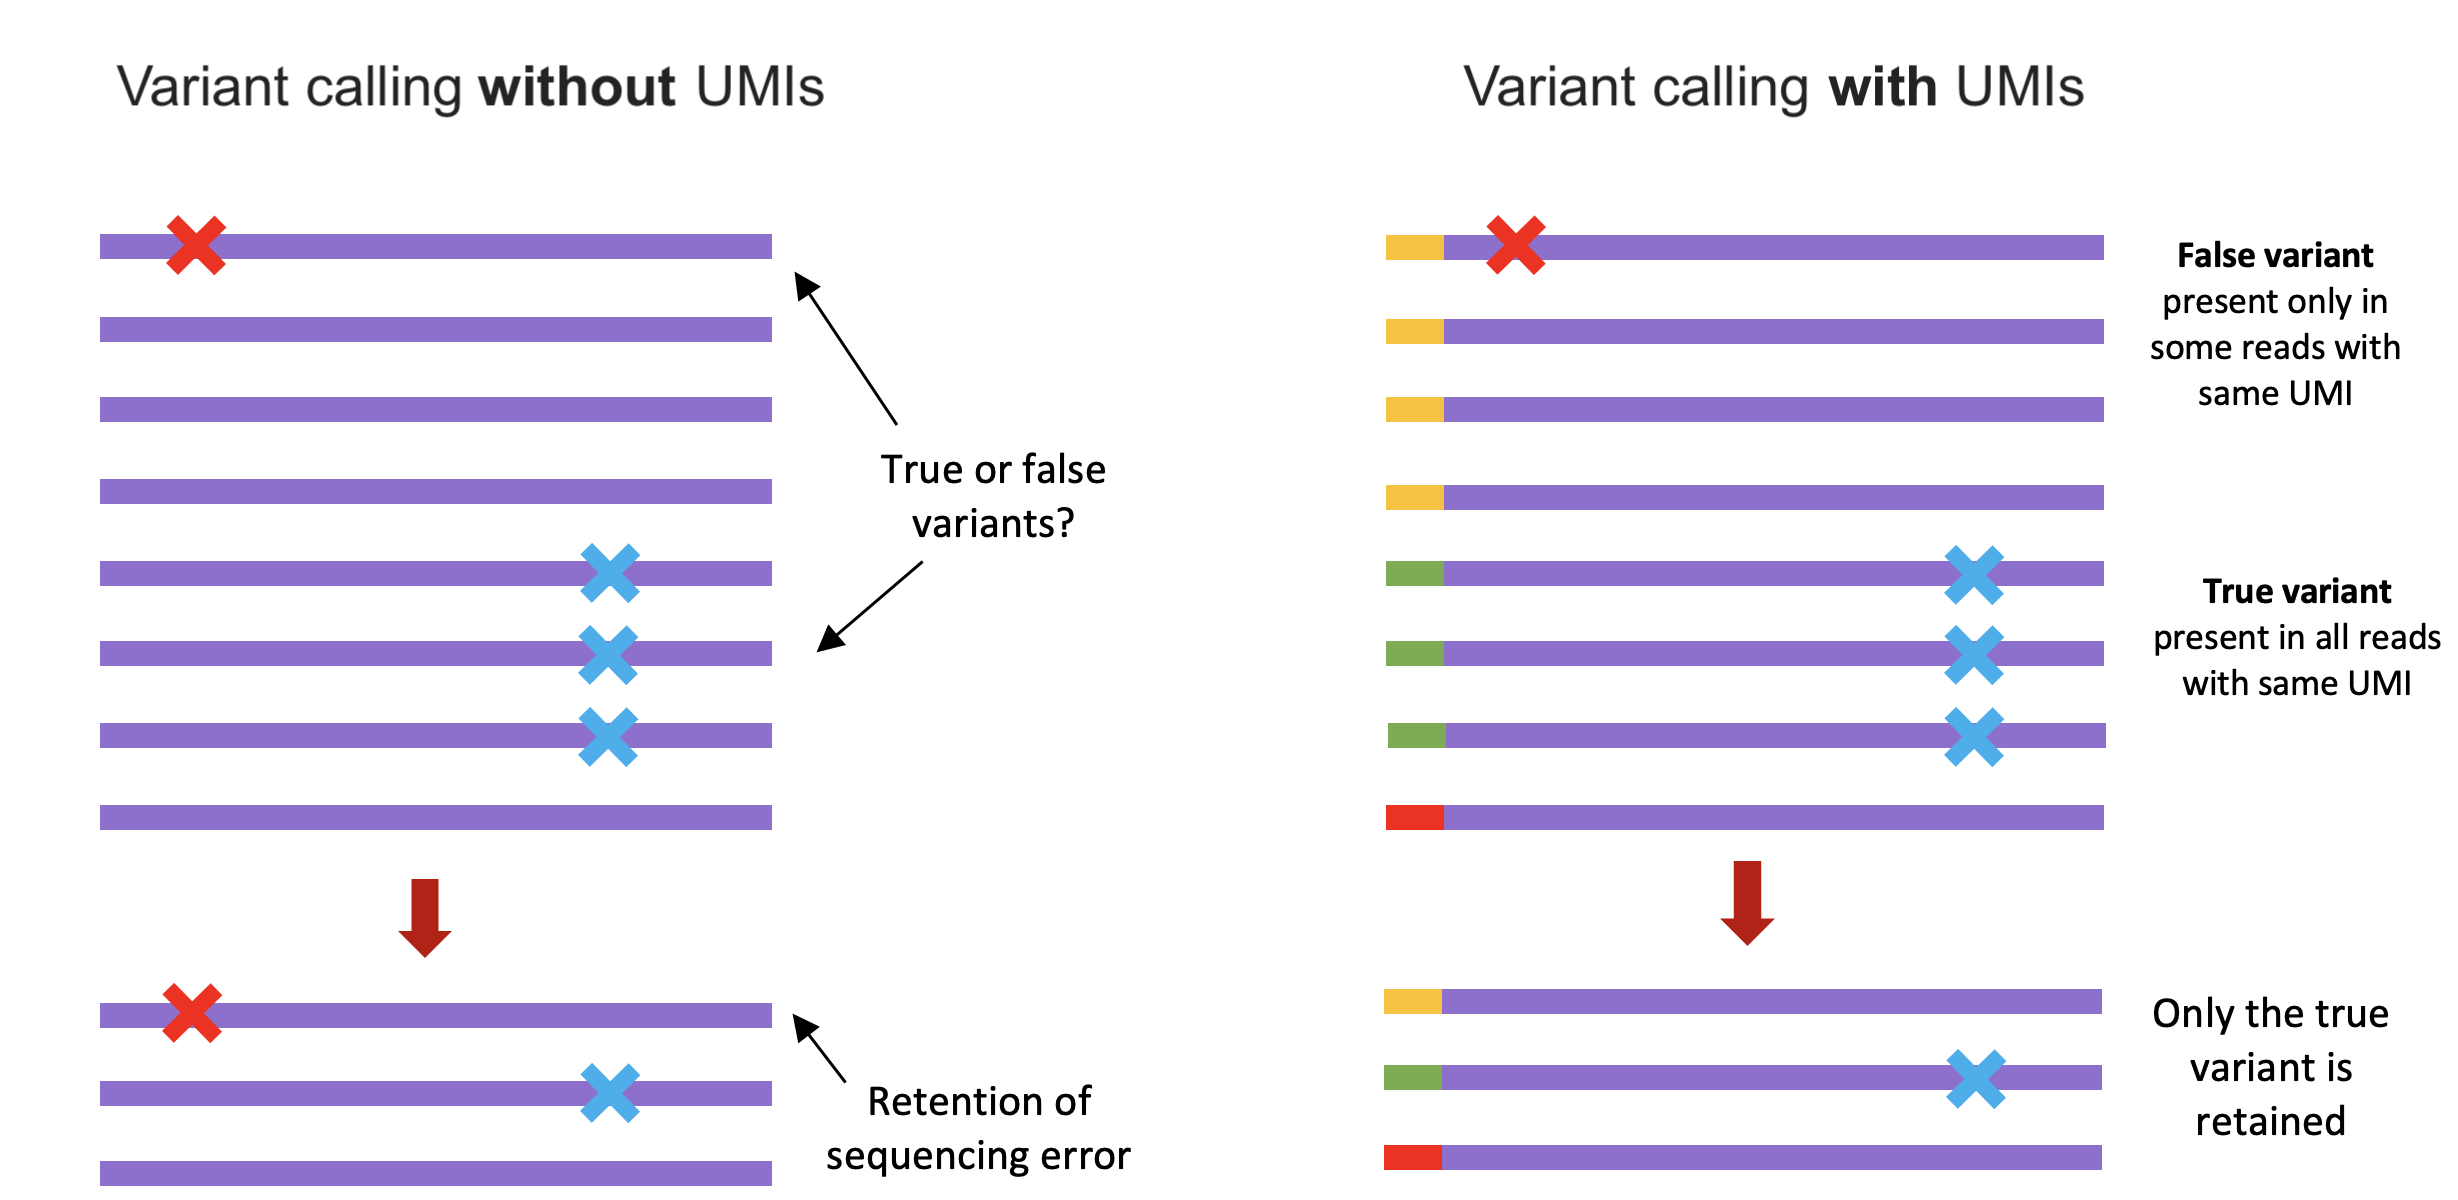
\includegraphics[width = \textwidth]{figs/umi-variants.png}
\caption{Representación de variantes con y sin UMIs.}
\label{fig:umi-variantes}
\end{figure}

En el método conocido como \textbf{Duplex Sequencing}, se emplean UMIs distintos en ambos extremos del fragmento de ADN. De este modo, durante el análisis de consenso, se pueden identificar las posiciones que muestran concordancia entre ambas hebras y descartar los nucleótidos mutados por error (figura \ref{fig:umi-variantes}).

\begin{figure}[htbp]
\centering
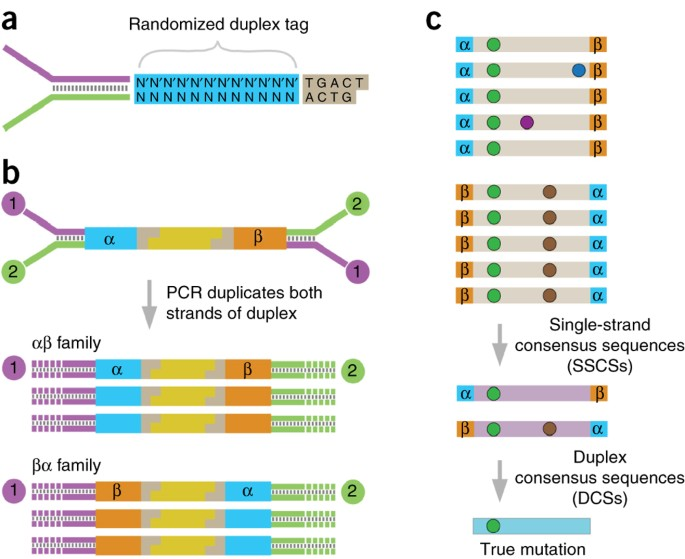
\includegraphics[width = 0.8\textwidth]{figs/duplex-sequencing.jpg}
\caption{Visión general de la secuenciación dúplex. (a) Esquema de un adaptador de secuenciación dúplex, que muestra la etiqueta aleatoria de doble cadena y la secuencia espaciadora invariante. (b) La ligación de los adaptadores con el ADN de la muestra da lugar a una secuencia única de 12 nt en ambos extremos de la molécula. La amplificación por PCR de cada cadena de un dúplex de ADN da lugar a dos productos de PCR distintos pero relacionados. (c) Las lecturas que comparten secuencias únicas de etiquetas $\alpha$ y $\beta$ se agrupan en familias de etiquetas de forma $\alpha \beta$ o $\beta \alpha$, y se crea un SSCS (single-strand consensus sequence) para cada familia de etiquetas. Las mutaciones son de tres tipos diferentes: errores de secuenciación (puntos azules o morados); errores de PCR de primera ronda (puntos marrones); mutaciones verdaderas (puntos verdes). La formación del SSCS elimina el primer tipo de error, pero no los errores de PCR de la primera ronda. La comparación de los SSCS de las familias emparejadas con etiquetas $\alpha \beta$ y $\beta \alpha$, genera un DCS (duplex consensus sequence), que elimina estos errores de PCR de primera ronda. Las mutaciones verdaderas se puntúan si y sólo si están presentes en la misma posición en ambas cadenas del ADN. "Detecting ultralow-frequency mutations by Duplex Sequencing, Nature, 2014"}
\end{figure}

Aunque los métodos basados en UMIs son altamente eficaces para detectar variantes de muy baja frecuencia, su uso es limitado debido a su alto costo, ya que requieren múltiples lecturas de la misma secuencia (mucha redundancia) para asegurar precisión (el consenso). Utilizando UMIs en un sólo una hebra, se necesita una redundancia de 1/30, y con duplex sequencing 1/200 para tener una buena representación. A veces, no interesa gastar tanto poder de secuenciación. 

\subsection{Adaptadores para secuenciación de célula única (single cell)}
En la secuenciación de célula única (Single Cell), se emplean adaptadores y primers que contienen identificadores UMIs específicos tanto para cada célula como para cada molécula de ADN. Esto permite diferenciar si las lecturas corresponden a una célula particular y, dentro de esa célula, a una molécula específica. En Single Cell, se utiliza un enfoque de consenso: las lecturas múltiples de la misma molécula permiten generar una secuencia de consenso para mejorar la precisión de los datos. A la hora de crear una biblioteca, esto es muy importante para aprovechar lo máximo posible el poder de secuenciación (presupuesto).

\begin{figure}[htbp]
\centering
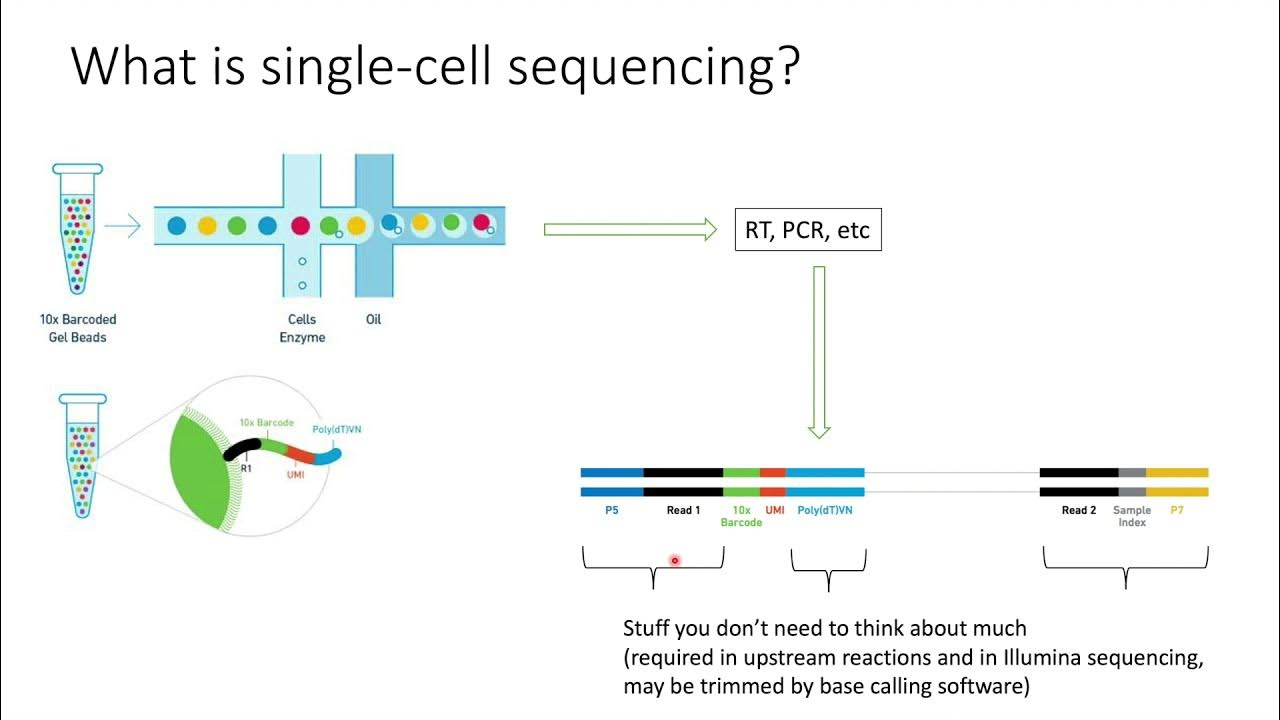
\includegraphics[width = 0.8\textwidth]{figs/single-cell-seq.jpg}
\caption{Descripción esquemática de la generación de GEM (gel beads-in-emulsions) y el código de barras con el flujo de trabajo del chip GEM-X. Los GEM se generan combinando perlas de gel con código de barras, una mezcla maestra que contiene células y aceite de partición en un chip GEM-X 3' o 5'. Para lograr una resolución unicelular, las células se suministran a una dilución límite, de modo que la mayoría ($\approx$90-99\%) de los GEM generados no contienen ninguna célula, mientras que el resto contiene en gran medida una sola célula.}
\end{figure}

La construcción de librerías en Single Cell se realiza mediante chips (que son como cajitas) que permiten el paso de flujo de células individuales junto con una especie de liposomas que contienen la mezcla de PCR. Cada mezcla de PCR tiene adaptadores con un barcode específico de célula, pero diferentes barcodes de molécula. Esto permite identificar y diferenciar las células individuales entre sí.

%Glosario
\begin{table}[htbp]
\begin{mdframed}[backgroundcolor=black!10]
    \centering
\textbf{Glosario}
\begin{description}
\item[Adaptadores:] Moléculas cortas de ADN fabricadas artificialmente que se unen a fragmentos de ADN y se utilizan para unirse a la célula de flujo.
\item[Barcoding:] El proceso de identificar muestras de ADN añadiendo índices a los fragmentos de ADN durante la preparación de la librería.
\item[Índice:] Molécula corta de ADN fabricada artificialmente que se utiliza para asignar códigos únicos a las muestras, lo que permite su identificación durante la secuenciación.
\item[Insert:] Fragmento de ADN entre dos adaptadores.
\item[Librería:] Una colección de fragmentos de ADN de tamaño aleatorio procedentes de una muestra determinada para ser secuenciados.
\item[Preparación de librería por ligación:] Método para ligar adaptadores a fragmentos de ADN para ser secuenciados.
\item[Multiplexing:] El proceso de añadir índices a los fragmentos de ADN durante la preparación de la librería.
\item[Oligos:] Moléculas de ADN artificial unidas a la célula de flujo que se unen por complementación a los adaptadores de los fragmentos de ADN.
\item[Lecturas/Reads:] Secuencias de pares de bases obtenidas de fragmentos de ADN.
\item[Preparación de librería por tagmentación:] Método para cortar y ligar adaptadores a fragmentos de ADN utilizando una enzima transposasa.
\item[Transposasa:] Enzima utilizada en la preparación de bibliotecas de marcaje para cortar y ligar adaptadores a fragmentos de ADN.
\end{description}
    \end{mdframed}
\end{table}

\section{Formatos de datos}
El formato de archivo usado por los alineadores es generalmente \textbf{FastQ} para las secuencias, aunque \textbf{Fast5} o \textbf{HDF5} también se emplean en algunos casos, especialmente en secuenciación de célula única (single cell), donde se necesita un mayor nivel de detalle (matrices de datos muy grandes) en el almacenamiento de datos.

Cuando se trabaja con alineadores, el proceso suele generar un perfil con picos que representan las bases detectadas, a cada uno de los cuales se le asigna el nombre de base. El alineador produce un archivo final dividido en campos que contiene: (i) el nombre de la $@$secuencia, (ii) la secuencia de bases asignadas, (iii) un + con posibles metadatos y (iv) la calidad de lectura de cada base en un formato codificado llamado \textbf{Phred33}, que usa caracteres ASCII para representar los valores de calidad.

En formatos antiguos, la cabecera de cada secuencia incluía datos detallados, como el nombre del instrumento de secuenciación, el identificador de la flowcell, las coordenadas X e Y del clúster, el número de la muestra y si es single-end(\_1) o pair-end(\_2). En el formato actual, esta información en la cabecera ha sido simplificada o se presenta de manera distinta, pero además presenta el nombre del UMI.

En cuanto al tipo de secuenciación, se distinguen dos tipos:
\begin{itemize}
\item \textbf{Single-end:} lee la secuencia en una sola dirección.
\item \textbf{Paired-end:} realiza lecturas en ambas direcciones, proporcionando información desde ambos extremos del fragmento de ADN. La secuenciación puede ser solapante (overlapping) para incrementar la evidencia de la secuencia, o no solapante (non-overlapping) cuando se busca mapear estructuras más amplias sin redundancia en los extremos.
\end{itemize}

\begin{figure}[htbp]
\centering
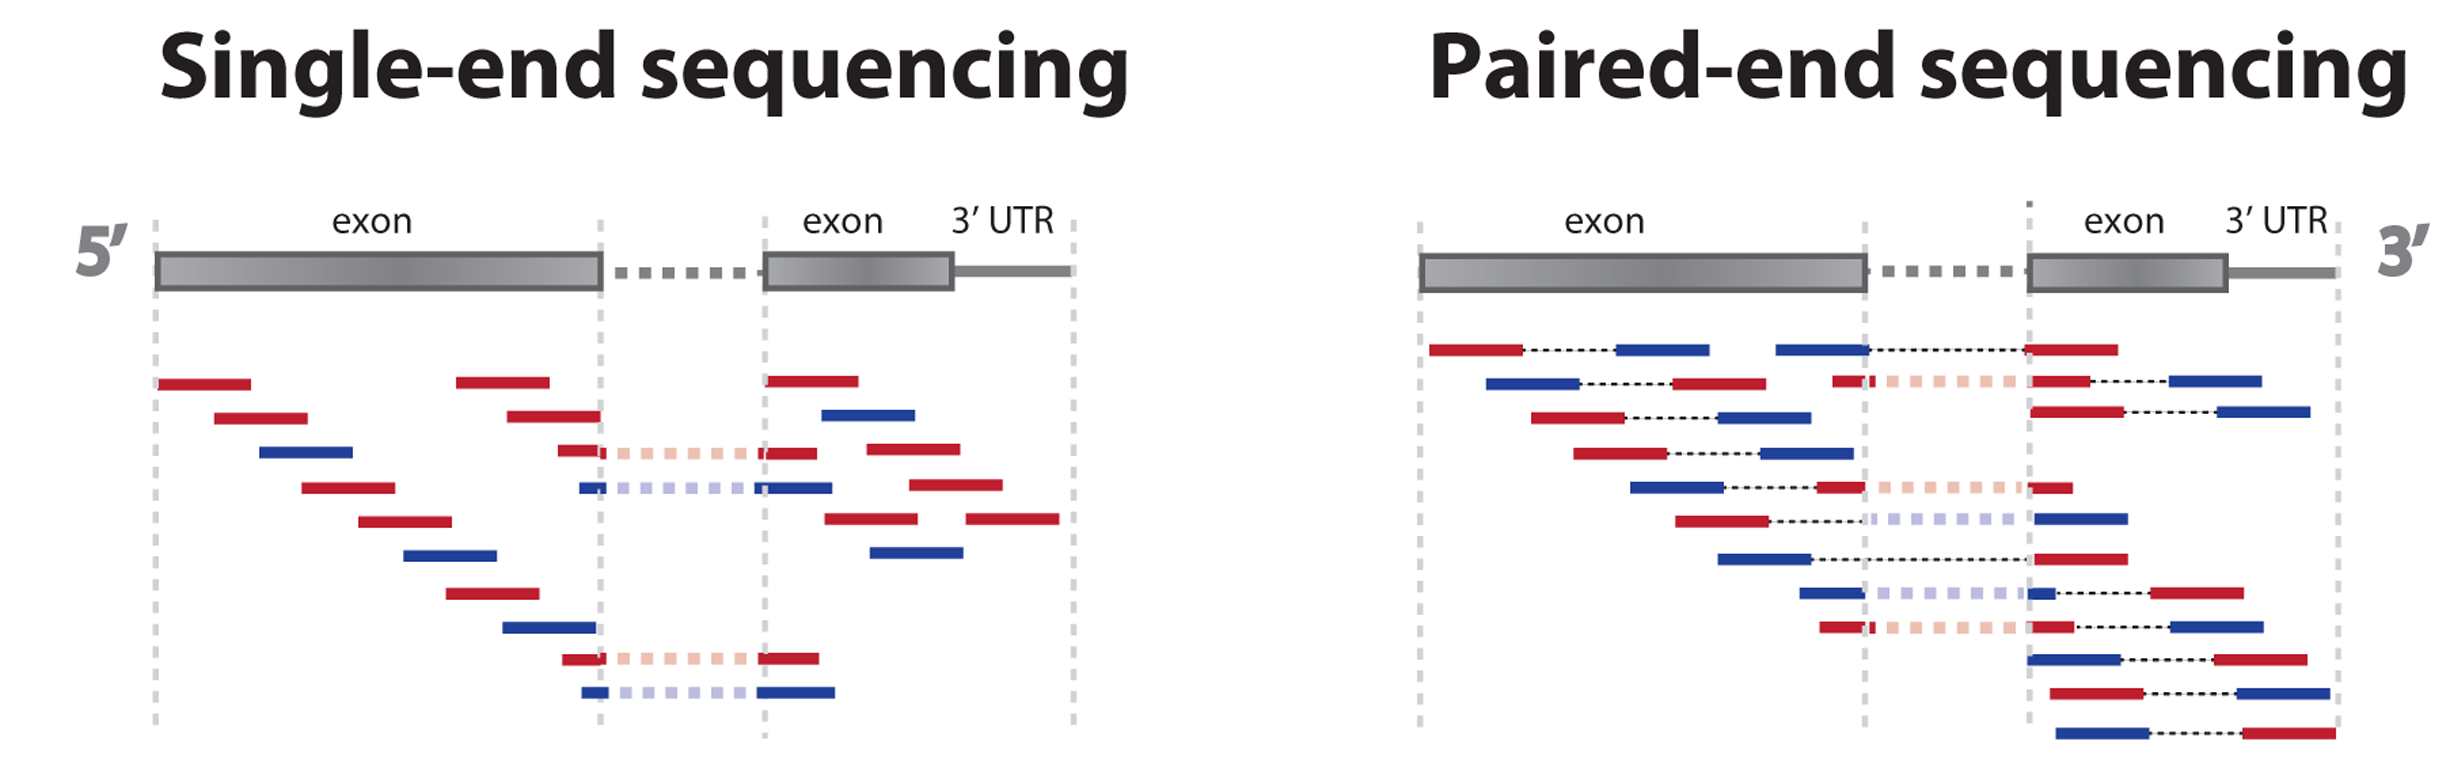
\includegraphics[width = 0.8\textwidth]{figs/singleEndVsPairedEnd.png}
\caption{Representación gráfica de la diferencia entre Single end y Paired end.}
\end{figure}

Durante un experimento de secuenciación, se utiliza un programa llamado \textbf{FastQC} para evaluar la calidad de las bases a lo largo de la lectura mediante una métrica llamada \textbf{Q score}. La visualización de estos resultados suele hacerse a través de diagramas de barras y cajas. Normalmente, la calidad de las bases tiende a disminuir conforme avanzan los ciclos de lectura, pero debe mantenerse dentro de un rango confiable.

\begin{figure}[htbp]
\centering
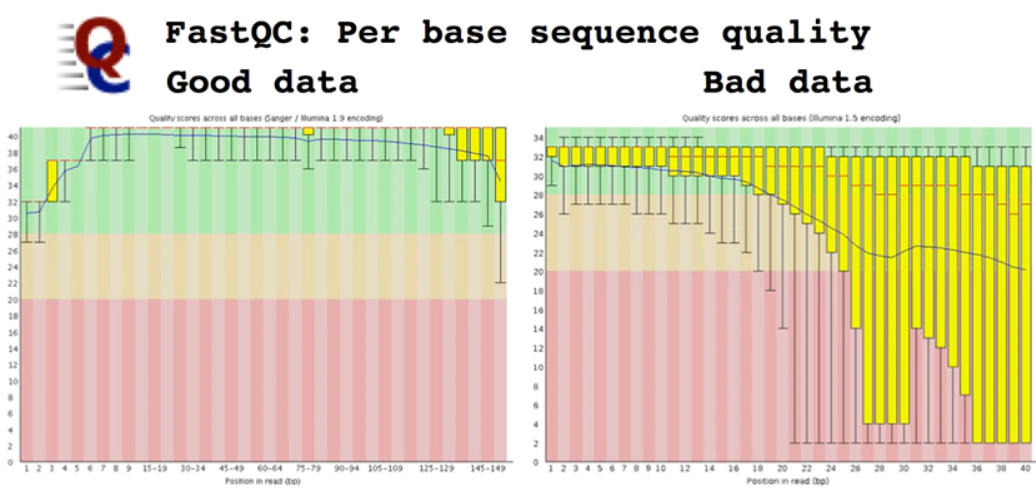
\includegraphics[width = \textwidth]{figs/good-bad-fastq.png}
\caption{La calidad de la secuencia por base, que representa la puntuación Q de la secuencia en crudo, se lee como un gráfico de caja para cada ciclo. Cuanto más alto, mejor, y en la mayoría de los ciclos se observa un descenso característico de la calidad.}
\end{figure}

FastQC proporciona varias métricas clave para evaluar la calidad: 
\begin{itemize} 
\item \textbf{Calidad promedio por secuencia}: muestra la calidad media de las bases en cada posición a lo largo de todas las secuencias. 
\item \textbf{Proporciones de bases por posición}: indica la proporción de bases (A, T, C, G) en cada posición. 
\item \textbf{Contenido de bases por posición}: permite identificar cualquier sesgo en el contenido de bases a lo largo de la secuencia. 
\item \textbf{Contenido GC:} al inicio de la secuenciación, puede haber una variación en el contenido GC debido a la secuencia de los adaptadores, pero si se estabiliza después de las primeras bases, indica una secuenciación correcta y se pueden cortar los primeros nucleótidos. 
\end{itemize}

\section{Preprocesamiento y genomas de referencia (FASTA)} 
El preprocesamiento de las lecturas aumenta la calidad de las secuencias, mejora el mapeo en la referencia, elimina posibles contaminantes y sesgos, y descarta segmentos no informativos.

Las secuencias generadas se comparan con \textbf{genomas de referencia}, que generalmente están en formato \textbf{FASTA}. En estos archivos, los nucleótidos están representados según el código IUPAC para permitir una representación estándar de variaciones entre individuos. Históricamente, los genomas de referencia se creaban con la información genética de un solo individuo. Sin embargo, hoy en día, se basan en el consenso de los genomas de múltiples individuos, lo que permite identificar variantes y posiciones con alta confianza que difieren entre individuos; por ello, la necesidad de usar el código IUPAC.

Los genomas de referencia y sus anotaciones se pueden encontrar en sitios como \href{https://hgdownload.soe.ucsc.edu/downloads.html}{UCSC Genome Browser}. Es importante tener en cuenta las diferencias en las anotaciones genómicas entre repositorios europeos y americanos, ya que pueden variar en la numeración y anotación de los cromosomas.

El formato FASTA se compone de dos líneas consecutivas:
\begin{itemize}
\item “>” Nombre de la secuencia y descripción opcional
\item Línea(s) con la secuencia completa
\end{itemize}
Aunque puede haber sólo una secuencia por archivo, es común que haya varias secuencias en el mismo archivo (multifasta). Y cuenta con varias extensiones (.fasta, .fas, .fa, .fna, .fsa).

\section{Alineamientos y mapeo}
El alineamiento es el proceso de comparar secuencias de ADN, ARN o proteínas para identificar regiones de similitud, lo cual puede revelar relaciones funcionales, estructurales o evolutivas entre las secuencias. Los objetivos principales del alineamiento son:
\begin{itemize}
\item Determinar el grado de homología para inferir relaciones filogenéticas
\item Identificar dominios funcionales
\item Comparar el gen con sus productos asociados
\item Encontrar posiciones homólogas entre secuencias
\item Identificar diferencias entre secuencias similares
\end{itemize}

\subsection{Alineamiento vs Mapeo}
Aunque a menudo se usan indistintamente, el alineamiento y el mapeo tienen diferencias importantes:
\begin{itemize}
\item \textbf{Alineamiento:} Cada posición de la secuencia de consulta se compara exhaustivamente con una secuencia de referencia para evaluar su precisión en cada sitio.
\item \textbf{Mapeo:} El objetivo es encontrar los loci más probables en la referencia donde una secuencia podría alinearse, priorizando eficiencia en velocidad y memoria. Es decir, encontrar la posición en la que se encuentra una secuencia lo más rápido posible.
\end{itemize}

Existen programas diseñados específicamente para el mapeo, llamados alineadores de lectura corta, que permiten configuraciones de mapeo como mapeo único, mapeo múltiple o mapeo con calidades parciales. Intentan ser rápidos y eficientes con el uso de la memoria. Dependiendo del tipo de secuenciación, se emplean diferentes alineadores:
\begin{itemize}
\item \textbf{Para ADN:} Novoalign, Bowtie2, BWA
\item \textbf{Para ARN:} RSEM, Salmon, Sleuth
\end{itemize}

\subsection{Algoritmos de mapeo por hashing}
El mapeo inicia con una etapa de \textbf{indexación del genoma}, un proceso intensivo en tiempo y memoria que se realiza solo una vez por genoma de referencia y por programa. En esta fase, los algoritmos de alineamiento utilizan técnicas como \textbf{hashing} o \textbf{índices} basados en \textbf{k-mers} (subsecuencias de longitud fija). Con una ventana móvil, se anotan las posiciones de cada k-mer en la secuencia de referencia.

Posteriormente, las lecturas se comparan con el diccionario de k-mers para localizar sus posiciones sin usar una ventana móvil adicional. A continuación, se construye un "árbol de posibilidades" que evalúa la compatibilidad de cada lectura con la referencia. Si una mutación en la lectura no coincide con la referencia, el k-mer no estará en el índice, y se buscarán los k-mers más cercanos, evaluando la mapping quality según el número de errores (mismatches) y la distancia de edición. El objetivo es minimizar los gaps (espacios sin coincidencias) para mejorar la precisión del alineamiento.

\begin{figure}[htbp]
\centering
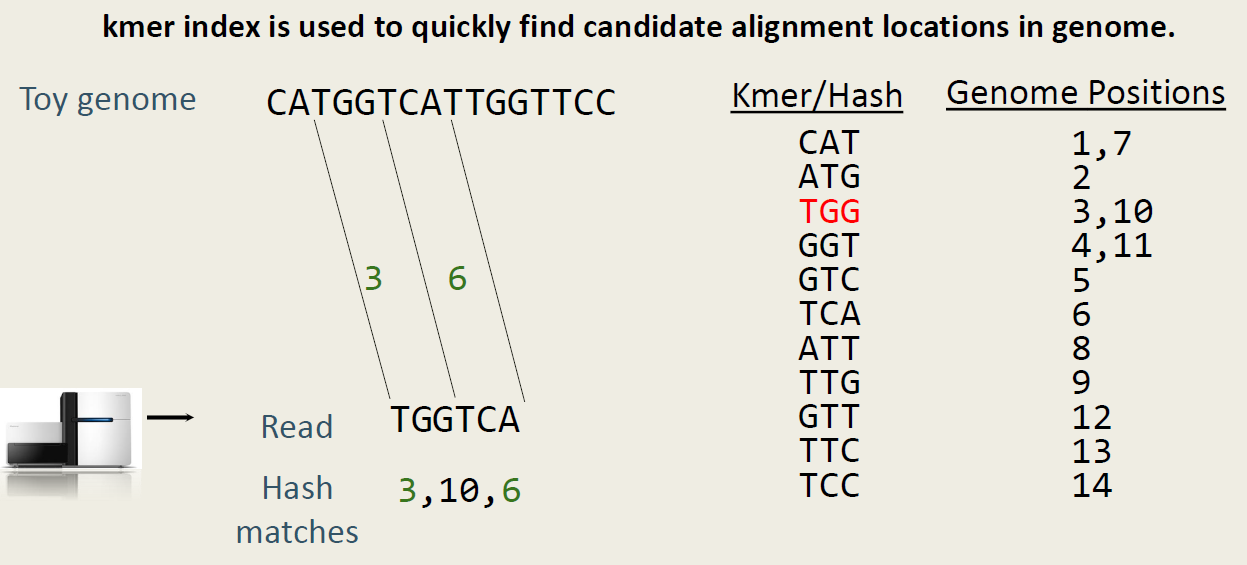
\includegraphics[width = \textwidth]{figs/hash-mapping.png}
\caption{Mapeado basados en hash o índices. El primer paso es obtener el hash o índice del genoma de referencia completo. A continuación, se utilizan esos índices para mapear (es decir, encontrar sitios de alineamiento) las lecturas.}
\end{figure}

\subsection{Transformación de Burrows-Wheeler (BWT)}
La \textbf{transformación de Burrows-Wheeler} es un método de compresión que permite realizar búsquedas rápidas de alineamiento en el genoma de referencia, optimizando el rendimiento de los alineadores.

\subsection{Estados de lecturas post-mapeo y mapping quality}
Una vez mapeadas las lecturas al genoma de referencia, se pueden obtener los distintos estados:
\begin{itemize}
\item \textbf{Lecturas no mapeadas:} No encuentran ninguna coincidencia en la referencia.
\item \textbf{Lecturas con mapeo único:} Mapean la secuencia en una sola posición de la referencia. Normalmente se trabaja con estas lecturas.
\item \textbf{Lecturas con mapeo múltiple (multimappers):} Ha mapeado varias posiciones. Se distinguen mapeos primarios y secundarios en función de la puntuación de mapeo. Se puede concatenar con técnicas heurísticas.
\end{itemize}

Existen opciones para reportar todos los alineamientos, solo los mejores, o aquellos que superan un umbral de calidad específico.

La calidad de mapeo usa la misma escala Phred33 que las calidades de lectura, y los resultados de alineación se almacenan en formatos SAM, BAM o CRAM:
\begin{itemize}
\item \textbf{SAM:} Formato de texto plano que se puede leer por la terminal.
\item \textbf{BAM:} Versión binaria de SAM. Normalmente se utiliza el BAM porque está más comprimido y es más portable.
\item \textbf{CRAM:} Similar a BAM, pero usado principalmente por el ENA-EBI, optimizado para almacenar una cantidad masiva de datos de forma compacta. Almacena las variantes de nucleótidos (mismatch call) de una secuencia con respecto a una secuencia de referencia y su posición (mismatch position) con respecto al inicio de la secuencia que contiene la variante (start offsets).
\end{itemize}

Los formatos SAM y BAM se pueden convertir entre sí mediante la herramienta \textbf{samtools}, que permite especificar el grado de compresión.

La cabecera del archivo S/BAM comienza con todas las líneas que empiezan por $@$ que almacena metadatos como la versión de SAM, la ordenación, los contigs y la información general del mapeo. A continuación se muestran los datos de la secuencia.
\begin{figure}[htbp]
\centering
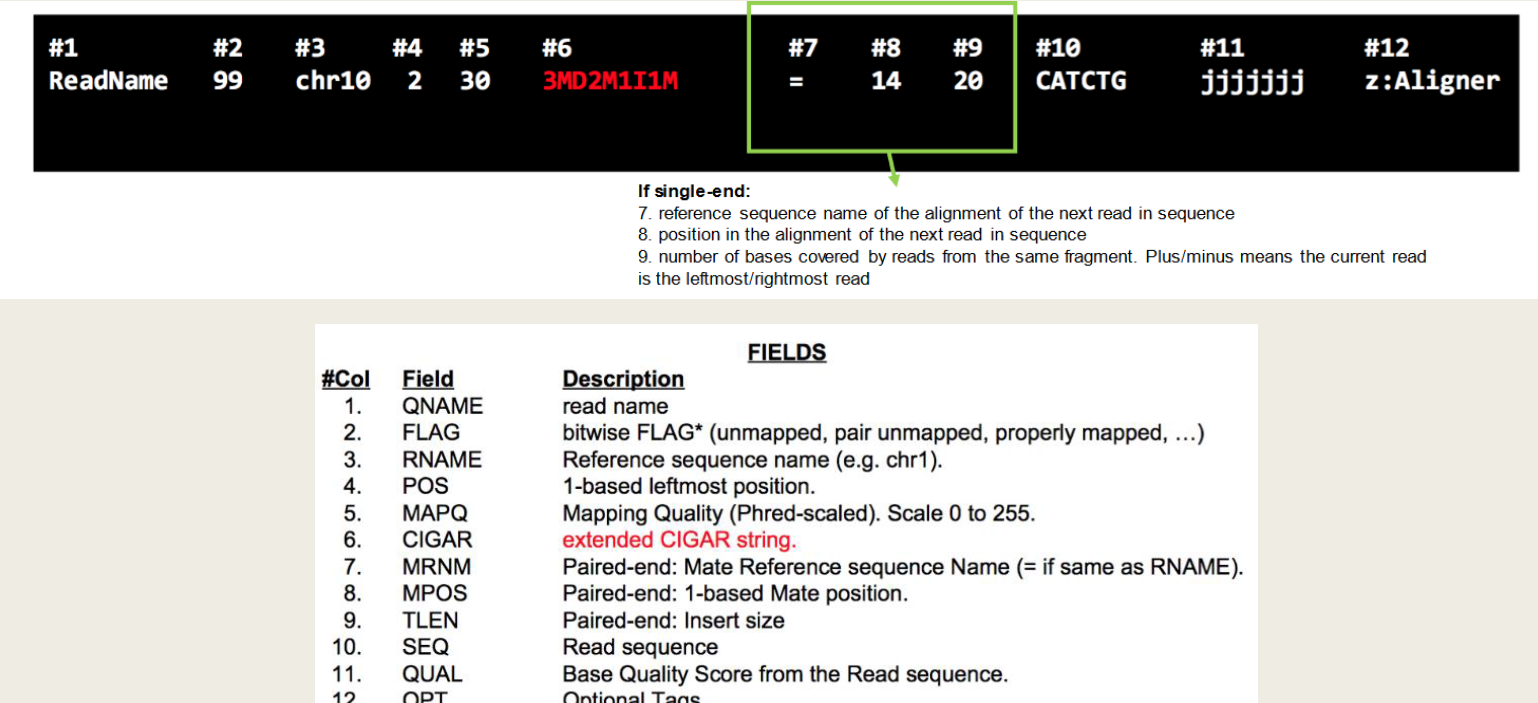
\includegraphics[width = \textwidth]{figs/sam-header.png}
\caption{Campos que incluye la cabecera de los ficheros SAM y BAM.}
\end{figure}

Los datos de alineación incluyen: 
\begin{itemize} 
\item QName: Nombre de la lectura 
\item Flag: Indica si la lectura está mapeada o no, entre otras propiedades. Sigue la codificación de \href{https://broadinstitute.github.io/picard/explain-flags.html}{picard}.
\item RName: Cromosoma donde se ha mapeado la lectura. 
\item Pos: Posición inicial del mapeado en el cromosoma 
\item MapQ: Calidad de mapeo 
\item CIGAR string: resumen del mapeado y alineamiento. Codifica el número de los tipos de eventos en el alineamiento (match, mismatch, inserciones, deleciones). Por ejemplo, un CIGAR de 3M1D2M1I1M indica que hay 3 match, 1 deleción, 2 match, 1 inserción y 1 match.
\item Información sobre el mapeo del par: En caso de secuenciación paired-end, se incluye la ubicación de la pareja de la lectura. 
\end{itemize}

%06/11 - Álvaro Serrano
\subsection{Otros formatos de ficheros en bioinformática}
\paragraph{Bed para intervalos}
Este formato da información de coordenadas. Tiene 3 columnas obligatorias: cromosoma, posición de inicio (0 based) y posición de fin (1 based). Estas posiciones se pueden restar para obtener el tamaño del fragmento. Bed es un formato abierto que puede incluir otras columnas: nombre, score, strand, etc. Estos ficheros son de texto plano, aunque tienen la extensión .bed. 

\paragraph{VCF para llamada de variantes}
Las variantes son posiciones en el genoma que se marcan como mutadas. Tiene una cabecera que empieza con una doble almohadilla. Es un fichero de texto plano, que se puede binarizar en un fichero bcf. Dentro del cuerpo, las columnas son cromosoma, posición de la mutación, ID, nucleótido en la referencia, alternativa (nucleótido observado en la mutación), calidad (profundidad a la que se ha secuenciado, es decir, veces que se ha secuenciado una determinada posición), filtro , información adicional, tipo de formato y muestras. También aporta información sobre la fase, es decir, si una misma lectura detecta varias mutaciones.

\paragraph{GTF y GFF para transcriptomas de referencia} 
Estos archivos contienen anotaciones de elementos (secuencia codificante, non-coding RNA, etc) referidos al genoma, por lo que es útil para experimentos de transcriptómica. Cada característica está en una fila con nueve columnas separadas por tabuladores: nombre de la secuencia, fuente, característica, posición de inicio y de fin (ambas basadas en 1), score, strand, frame y atributos. 

\paragraph{CSV y TSV para cuentas}
No hay especificaciones de formato, ni límites en cuanto a la dimensión de la matriz. Son ficheros tabulares estándares. Es importante tener buenas prácticas, es decir, utilizar nombres intuitivos para columnas y filas, y no utilizar espacios, si no puntos o barras bajas. En las filas se guardan las observaciones, y las columnas las características. 

\chapter{Secuenciación de tercera generación}
La secuenciación de segunda generación, como los métodos basados en Illumina, permite obtener lecturas pequeñas (de alrededor de 100-300 pb) y de alta precisión, pero presenta limitaciones al enfrentar regiones genómicas complejas, como las altamente repetitivas, debido a la longitud de las lecturas. La secuenciación de tercera generación surge para superar estas limitaciones, proporcionando lecturas más largas (de varias kilobases) que permiten el análisis detallado de variantes estructurales, lo cual es esencial para estudios de genómica estructural y ensamblaje de genomas complejos.

Se distinguen dos enfoques principales en la secuenciación de tercera generación:
\begin{itemize}
\item \textbf{Secuenciación de molécula única:} secuencia cada molécula individual sin amplificación clonal, reduciendo así el sesgo introducido por técnicas de PCR. Destacan PacBio y Oxford Nanopore, cada uno con sus características particulares en cuanto a precisión, velocidad y métodos de detección.
\item \textbf{Aproximaciones sintéticas (basadas en Illumina):} permiten reconstruir secuencias largas a partir de lecturas cortas mediante ensamblaje. Estas no se consideran tercera generación en sentido estricto, pero comparten ciertos objetivos en cuanto a mejorar la resolución de lecturas largas (se habla de pseudotercera generación).
\end{itemize}

\section{Secuenciación de molécula única a tiempo real - PacBio}
La tecnología de PacBio (Pacific Biosciences) emplea una única molécula de ADN de longitud variable, generalmente en el rango de varias kilobases. Se preparan fragmentos circulares de ADN al añadir estructuras químicas en forma de horquilla en los extremos, lo que permite la circularización de la molécula y una lectura continua de la secuencia.

El secuenciador PacBio utiliza una flowcell con pocillos que contienen cámaras donde se detectan señales de fluorescencia para identificar los nucleótidos incorporados en tiempo real. Este proceso funciona gracias a una polimerasa anclada en cada pocillo que, al añadir nucleótidos marcados con fluorescencia, permite que la cámara capture el cambio y lea la secuencia. La velocidad de secuenciación es de aproximadamente 3 bases por segundo.

Cada pocillo secuencia una molécula única no amplificada que proviene directamente del organismo a estudiar. Al estar la molécula circularizada, la secuenciación puede realizarse de manera continua: la polimerasa desnaturaliza la cadena, incorpora nucleótidos y la cadena sintetizada se deshibrida, permitiendo múltiples pasadas sobre la misma región.

\begin{figure}[htbp]
\centering
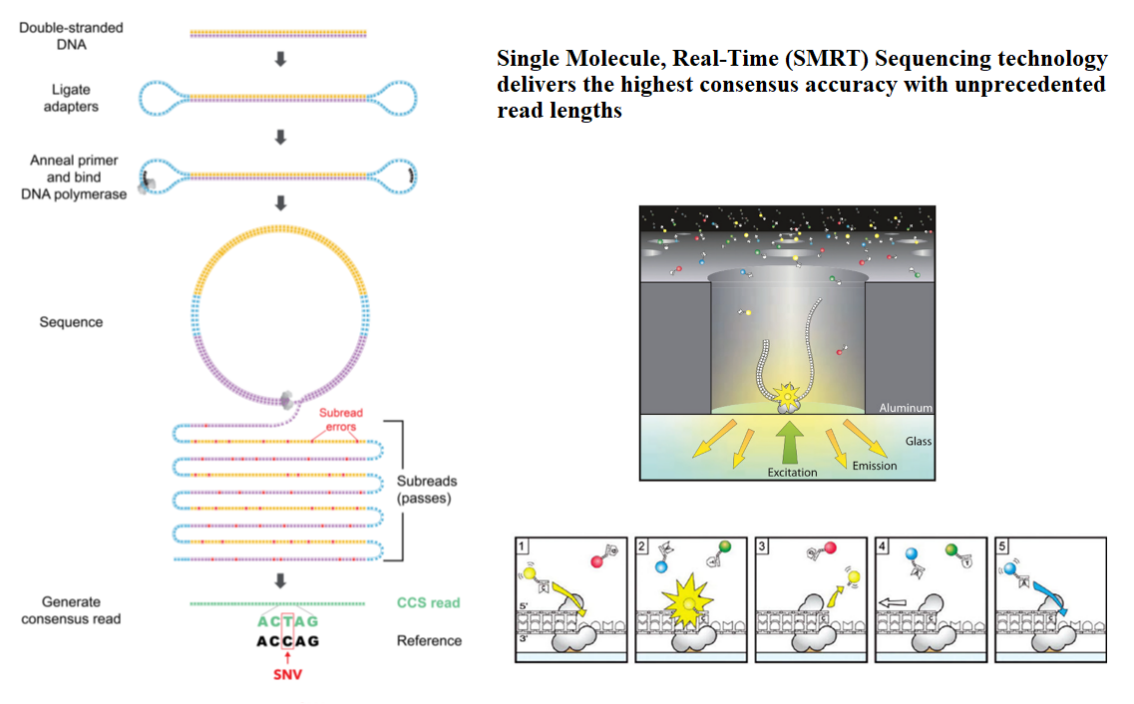
\includegraphics[width = \textwidth]{figs/pacbio.png}
\caption{La plataforma de secuenciación PacBio es una plataforma de secuenciación de lectura larga, también conocida como una de las tecnologías de secuenciación de tercera generación (TGS). La tecnología central, la molécula única en tiempo real (SMRT), permite generar lecturas de decenas de kilobases de longitud. Sobre la base de la «secuenciación por síntesis», la resolución de nucleótidos individuales se consigue mediante la guía de ondas de modo cero (ZMW), en la que sólo se ilumina un volumen limitado en la parte inferior (el lugar de síntesis de la molécula). Además, la secuenciación SMRT evita en gran medida el sesgo de secuencia específica en el sistema NGS, ya que la mayoría de los pasos de amplificación PCR no son necesarios en el proceso de construcción de bibliotecas.}
\end{figure}

PacBio permite dos enfoques distintos:
\begin{itemize}
\item \textbf{Circular Long Templates (CLT):} se secuencian fragmentos largos una sola vez para capturar grandes porciones de información estructural del ADN.
\item \textbf{Circular Consensus Sequencing (CCS):} se secuencian fragmentos más cortos repetidamente, lo que permite asegurar la precisión en cada posición al promediar múltiples lecturas del mismo fragmento.
\end{itemize}

Este método es especialmente útil en el ensamblaje de genomas debido a la longitud de las lecturas. La calidad en el modo CCS puede alcanzar valores elevados (Q50), aunque en regiones de homopolímeros extensos puede haber dificultades en la discriminación precisa de nucleótidos individuales, generando posibles discrepancias con la secuencia real si solo se realiza una pasada.
%PacBio Sequencing - How it works YouTube

\section{Secuenciación por Nanoporos - Oxford Nanopore Technology (ONT)}
La tecnología de secuenciación por nanoporos, desarrollada por Oxford Nanopore, utiliza proteínas alfa-hemolisinas que forman poros a través de los cuales pasa una cadena de ADN, generando una señal eléctrica que permite identificar los nucleótidos en tiempo real. Esta señal, medida como una interferencia de corriente (diferencia de potencial), permite la identificación directa de bases sin la necesidad de etiquetas de fluorescencia, lo cual distingue a ONT de otros métodos de secuenciación.

En el caso de ADN de doble cadena, el sistema emplea una proteína motora que desnaturaliza el ADN, permitiendo que solo una cadena pase a través del poro. A medida que cada nucleótido atraviesa el poro, la interferencia generada, conocida como \textbf{"squiggle" o garabato}, se mide y se asocia con una secuencia de bases. Para traducir esta señal en una secuencia, se comparan patrones de squiggles generados experimentalmente con secuencias sintéticas (o "similares"), lo que permite identificar los nucleótidos en cada posición.

\begin{figure}[htbp]
\centering
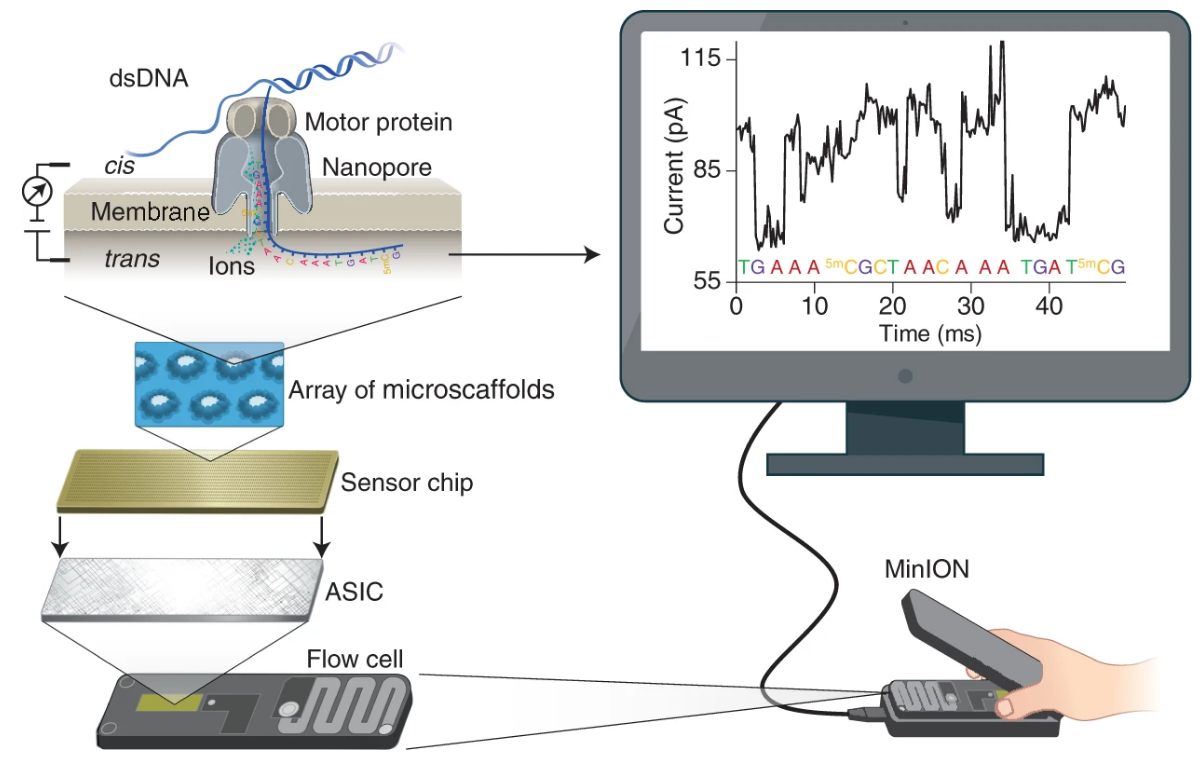
\includegraphics[width = 0.8\textwidth]{figs/nanopore.png}
\caption{Una celda de flujo MinION contiene 512 canales con 4 nanoporos en cada canal, para un total de 2.048 nanoporos utilizados para secuenciar ADN o ARN. Los pocillos se insertan en una membrana de polímero resistente a la electricidad soportada por una matriz de microesqueletos conectados a un chip sensor. Cada canal se asocia a un electrodo independiente en el chip sensor y es controlado y medido individualmente por el circuito de integración de aplicaciones específicas (ASIC). La corriente iónica pasa a través del nanoporo porque se aplica un voltaje constante a través de la membrana, donde el lado trans está cargado positivamente. Bajo el control de una proteína motora, primero se desenrolla una molécula de ADN de doble cadena (o un dúplex híbrido de ARN-ADN) y, a continuación, el ADN o ARN monocatenario con carga negativa se desplaza a través del nanoporo, impulsado por el voltaje. A medida que los nucleótidos atraviesan el nanoporo, se mide un cambio de corriente característico que se utiliza para determinar el tipo de nucleótido correspondiente a unas 450 bases por s. "Nanopore sequencing technology, bioinformatics and applications, Nature, 2021"}
\end{figure}

El sistema ONT incluye una región denominada \textbf{k-mero} en el poro, que es el área de mayor estrechamiento y donde la señal de corriente es más intensa. Esto permite capturar mayor información y mejorar la precisión de la secuenciación, aunque este proceso es complejo y requiere el uso de algoritmos avanzados, como redes neuronales, para categorizar las señales y asignar los nucleótidos correspondientes.

La tecnología de ONT es altamente precisa y tiene la capacidad de secuenciar hasta 500 megabases, con un tamaño promedio de lectura de entre 4-6 kilobases. Sin embargo, la calidad de las lecturas puede ser inferior a otros métodos de secuenciación, con una precisión de aproximadamente 92-93\%, debido en parte a las limitaciones en la resolución de homopolímeros y otras regiones repetitivas.

A pesar de estas limitaciones, la tecnología ONT es portátil, escalable y rápida, lo que permite lecturas largas sin necesidad de amplificación por PCR. La tecnología admite modificaciones químicas en el ADN, como la adición de un "hairpin" (estructura en horquilla), que permite secuenciar ambas hebras del ADN en un solo paso.

Las principales desventajas de la secuenciación por nanoporos son la elevada tasa de error y las dificultades en regiones con homopolímeros extensos, así como su dependencia de "training sets" (conjuntos de datos de entrenamiento) actualizados para mejorar la precisión en el análisis de secuencias complejas.

\section{Consideraciones generales sobre la secuenciación de tercera generación}
Las técnicas de secuenciación de tercera generación han revolucionado el campo de la genómica estructural, permitiendo lecturas largas que facilitan el ensamblaje de genomas completos y el análisis de variaciones estructurales. Sin embargo, en comparación con la secuenciación de segunda generación, presentan una menor precisión en general. A medida que se integran algoritmos de inteligencia artificial y técnicas avanzadas de procesamiento de señales, la precisión de estas tecnologías sigue mejorando.

Un desafío específico en estas tecnologías es la susceptibilidad de las moléculas únicas a la adición de múltiples nucleótidos, lo que puede generar errores en homopolímeros y regiones complejas del ADN.

\section{Resumen}
La secuenciación de tercera generación permite secuenciar templates más largos, siendo así mejor para variantes estructurales. Además, no es necesaria la amplificación clonal. En \textbf{PacBio}, se utilizan templates circularizados. La polimerasa incorpora dNTPs con fluoróforos que se capturan por una cámara directamente cuando se unen. Es muy rápido (3 bases por segundo), pero sufre en regiones con homopolímeros. Se secuencian los templates largos una vez con una tasa de error alta o templates cortos varias veces para obtener el consenso. En \textbf{Nanopore}, se comprueba directamente la composición de un ssDNA mediante la interpretación de la interrupción de la corriente (el garabato o squiggle). Dentro del poro, la zona estrecha dtermina el k-mero. Éste sufre más con homopolímeros cuando el k-mero es más corto. Tiene una tasa de error alta, pero se está optimizando con machine learning. También puede haber problemas con bases modificadas. Los equipos son muy portables, lo que supone una gran ventaja.

\section{Quizz}
\begin{enumerate}
\item What is an advantage of hash table-based mapping?
\begin{itemize}
\item Allows alignment without reference
\item Requires less memory
\item Higher speed and efficiency
\item Only used with long reference genomes
\end{itemize}

Answer: Higher speed and efficiency

\item What does the variant allele frequency (VAF) mean?
\begin{itemize}
\item The number of observed reads that match a specific variant
\item The percentage of errors in a sequence
\item The number of sequences in a reference genome
\item The quality of the sequence in an alignment
\end{itemize}

Answer: The number of observed reads that match a specific variant

\item What does a high Phred Q value in quality scores mean?
\begin{itemize}
\item Higher probability of error
\item Higher accuracy in the called base
\item Low quality sequences
\item Systematic error in final bases
\end{itemize}

Answer: Hiher accuracy in the called base

\item What is an example of a short read aligner (SRA)?
\begin{itemize}
\item ClustalW
\item BWA
\item Excel
\item SnapGene
\end{itemize}

Answer: BWA

\item What does 'NGS' mean?
\begin{itemize}
\item Next Genomic Study
\item Next Generation Sequencing
\item Next Generation Science
\item Next Generation Studies
\end{itemize}

Answer: Next Generation Sequencing

\item What file format is used to represent DNA sequences with their quality scores?
\begin{itemize}
\item VCF
\item SAM
\item FASTQ
\item GFF
\end{itemize}

Answer: FASTQ

\item What does a GTF/GFF file describe in bioinformatics?
\begin{itemize}
\item DNA mutations
\item Genomic annotations
\item Sequence variants
\item Reference sequences
\end{itemize}

Answer: Genomic annotations

\item What is the goal of unique molecular identifiers (UMI)?
\begin{itemize}
\item Identify individual molecules and reduce PCR duplicates
\item Align reference DNA
\item Improve the VCF file format
\item Store alignment quality
\end{itemize}

Answer: Identify individual molecules and reduce PCR duplicates

\item What type of file is used to represent genomic coordinates in interval analysis?
\begin{itemize}
\item FASTA
\item BAM
\item BED
\item CRAM
\end{itemize}

Answer: BED

\item What type of format is commonly used to store the reference genome?
\begin{itemize}
\item FASTA
\item BED
\item BAM
\item SAM
\end{itemize}

Answer: FASTA

\item What do UMIs represent in sequencing?
\begin{itemize}
\item Duplication indicators
\item Unique molecular identifiers
\item Adapter sequences
\item Alignment marks
\end{itemize}

Answer: Unique molecular identifiers

\item What is the main purpose of a library in sample preparation?
\begin{itemize}
\item Store sequence data
\item Fragment DNA
\item Generate DNA fragments from a sample for sequencing
\item Calculate the quality of the sequence
\end{itemize}

Answer: Generate DNA fragments from a sample for sequencing

\item What component in a VCF file indicates the score assigned to a variant call?
\begin{itemize}
\item Chr
\item Qual
\item Pos
\item Alt
\end{itemize}

Answer: Qual

\item What is the BED format used for in bioinformatics?
\begin{itemize}
\item Store alignments
\item Represent genomic coordinates
\item Sequence DNA
\item Store quality data
\end{itemize}

Answer: Represent genomic coordinates

\item What file format is used to report genetic variations?
\begin{itemize}
\item SAM
\item FASTA
\item GTF
\item VCF
\end{itemize}

Answer: VCF

\item What is the Phred Q value if the probability of error is 1 in 100?
\begin{itemize}
\item 10
\item 20
\item 30
\item 40
\end{itemize}

Answer: 20

\item What technology uses real-time single-molecule sequencing?
\begin{itemize}
\item Illumina
\item PacBio
\item SOLiD
\item ABI
\end{itemize}

Answer: PacBio

\item What is the CIGAR line in a SAM/BAM file?
\begin{itemize}
\item An ASCII code line
\item A compressed representation of an alignment
\item The identification of the reference sequence
\item A metadata line
\end{itemize}

Answer: A compressed representation of an alignment

\item Which of the following is a characteristic of BAM files?
\begin{itemize}
\item They are human-readable text files
\item They are binary alingment files
\item They cannot be compressed
\item They are reference genome files
\end{itemize}

Answer: They are binary alignment files

\item What is the function of adapters in NGS?
\begin{itemize}
\item Sequence RNA fragments
\item Ligate DNA fragments to flow cells
\item Fragment DNA
\item Adjust the quality of the sequence
\end{itemize}

Answer: Ligate DNA fragments to flow cells

\item What is one of the mandatory columns in a VCF file?
\begin{itemize}
\item Qual
\item ID
\item REF
\item All of the above
\end{itemize}

Answer: All of the above

\item Which of the following options is NOT a stage in library preparation?
\begin{itemize}
\item Fragmentation
\item Ligate adapters
\item Mapping analysis
\item Purification
\end{itemize}

Answer: Mapping analysis

\item What file is a human-readable text format that contains sequence alignment information?
\begin{itemize}
\item SAM
\item BAM
\end{itemize}

Answer: SAM

\item What file is a human-readable text format that contains sequence alignment information?
\begin{itemize}
\item SAM
\item BAM
\item VCF
\item GFF
\end{itemize}

Answer: SAM

\item What is the main feature of nanopore sequencing?
\begin{itemize}
\item Ionic current monitoring to detect DNA composition
\item Use of fluorescent tags on each base
\item Low throughput
\item Only sequence RNA
\end{itemize}

Answer: Ionic current monitoring to detect DNA composition

\item What type of alignment is characteristic of NGS?
\begin{itemize}
\item Alignment based on long sequences
\item Short read alignment to a reference genome
\item Alignment with very low quality sequences
\item Alignment without the need for reference
\end{itemize}

Answer: Short read alignment to a reference genome

\item What library preparation method uses the transposase enzyme?
\begin{itemize}
\item Ligate adapters directly
\item Ligate UMIs
\item Tagmentation
\item Generate high-quality sequences
\end{itemize}

Answer: Tagmentation

\item What file is the binary version of a SAM file?
\begin{itemize}
\item CRAM
\item BAM
\item FASTA
\item CSV
\end{itemize}

Answer: BAM

\item What file is typically used to store tabular data in bioinformatics?
\begin{itemize}
\item CSV/TSV
\item BED
\item FASTA
\item CRAM
\end{itemize}

Answer: CSV/TSV

\item What is the main advantage of third-generation sequencing?
\begin{itemize}
\item Low accuracy
\item Long reads without template amplification
\item High speed without alignment
\item Low error rate in homopolymeric regions
\end{itemize}

Answer: Long reads without template amplification
\end{enumerate}

%aserrano@cnic.es
%08/11 - Tomás di Domenico
\chapter{Whole Genome Sequencing (WGS)}
\section{Introducción a Whole Genome Sequencing}
WGS implica secuenciar todo el genoma de telómero a telómero. Esto se debe a que antes no se solía secuenciar todo el genoma, si no algún panel o el exoma. Ahora, el genoma completo sí se está secuenciando por la disminución de los costes. 
\begin{itemize}
\item \textbf{Targeted panel sequencing}: como se selecciona un fragmento a secuenciar, se consigue una mayor cobertura por el mismo precio.
\item \textbf{Whole-exome sequencing (WES):} se secuencia todo el exoma, por lo que la cobertura es intermedia.
\item \textbf{Whole-genome sequencing (WGS):} se secuencia todo el genoma, pero con una cobertura menor.
\end{itemize}

Las ventajas de WGS es que no hay ADN "basura", y que mucha regulación ocurre en el genoma no codificante. Además, las variantes estructurales solo se ven con una perspectiva completa. En resumen, un WGS es la representación completa del genoma de un organismo. No obstante, no siempre se realiza WGS por temas económicos: los costes de secuenciación, los costes de almacenamiento y los costes de análisis. El exoma representa un 1\% del genoma, por lo que conseguir una mayor cobertura en WES es más barato que en WGS.

\begin{figure}[htbp]
\centering
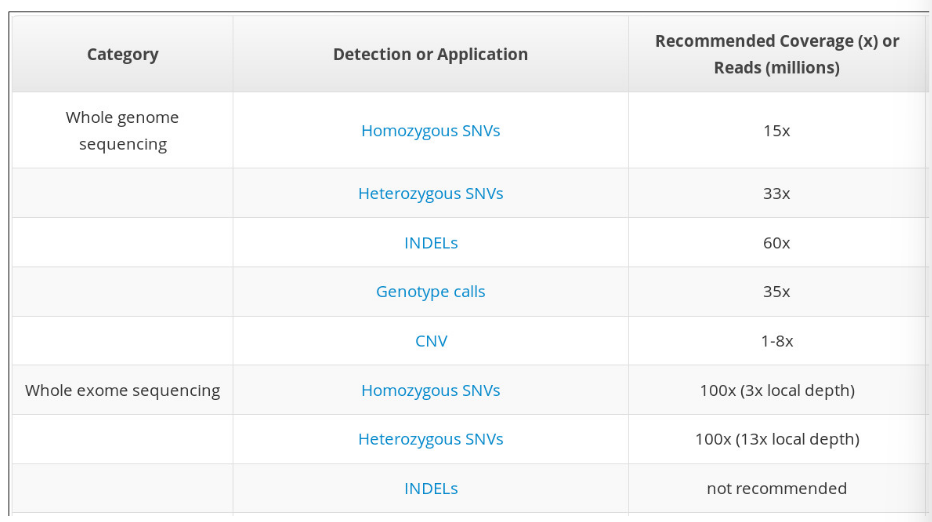
\includegraphics[width = 0.7\textwidth]{figs/wge-wgs.png}
\caption{Comparación de las coberturas recomendadas para WGE y WGS en base a su aplicación.}
\end{figure}

WGS tiene tres aplicaciones fundamentales:
\begin{itemize}
\item \textbf{Ensamblajes:} El ensamblaje de un genoma es una de las principales ventajas de poder secuenciar un genoma completo. Los ensamblajes basados en NGS implican reconstruir secuencias desde lecturas cortas, lo que es muy exigente computacionalmente. De las lecturas se forman los contigs, los cuales se ensamblan en scaffolds. Finalmente, los scaffolds se pueden ensamblar en pseudocromosomas y cromosomas. La generación de un genoma completo, pese a seguir siendo caro, ha reducido su coste desde el Proyecto Genoma Humano. Es importante poder hacer un ensamblado porque el genoma de referencia no es representativo por la diversidad natural y en algunos casos tiene muchos huecos.
\item \textbf{Genome-wide Association Studies (GWAS):} El análisis de variaciones a nivel genómico se puede realizar mediante la secuenciación de datos genómicos. No obstante, sigue habiendo problemas en cuanto a la relevancia y la estadística.
\item \textbf{Análisis de variantes estructurales:} La variación estructural, o la reorganización de partes del genoma de varias formas solo es posible capturarla mediante la secuenciación del genoma completo.
\end{itemize}

La principal limitación de NGS es que generan lecturas muy cortas, además de tener limitaciones intrínsecas por los métodos químicos que se utilizan a la hora de secuenciar. De estos métodos, el más popular es el de la secuenciación por síntesis, que es el que implementa Illumina en su secuenciación. Después de varias rondas de extensión y escaneado, las copias de la secuencia en un cluster empieza a descoordinarse, por lo que hay una limitación del tamaño de las lecturas. Esto es particularmente exigente cuando se trata de regiones que pueden estar repetidas a lo largo del genoma, ya que los ensamblajes pueden mostrar sesgos, dando lugar a huecos en los ensamblajes de referencia. Los genomas suelen ser muy repetitivos, pero hay distintos grados de repetitividad (simple y complejo). Así, no toda la parte repetitiva impide el ensamblaje, pero causa estragos.

\section{Práctica - lecturas cortas}
Ahora vamos a adquirir experiencia práctica con un ensamblaje de lecturas cortas y su análisis.
Como no tenemos tiempo ni recursos para trabajar con un genoma entero, trabajaremos con un fragmento amplificado por BAC del cromosoma 3 humano.
Utilizaremos ABySS para ensamblar un cromosoma artificial bacteriano (BAC) de 200 kbp utilizando un carril de lecturas paired-end de la plataforma Illumina. BWA-MEM se utiliza para alinear los contigs ensamblados con el genoma humano de referencia. IGV se utiliza para visualizar estas alineaciones y variantes.
Después de esta práctica, habremos aprendido a ensamblar un genoma pequeño, a utilizar BWA-MEM para alinear lecturas y contigs con un genoma de referencia, y a utilizar el navegador del genoma UCSC e IGV para visualizar estas alineaciones.

Los BAC pueden utilizarse para amplificar un determinado fragmento de ADN de interés dentro de bacterias. Se utilizó mucho para generar el genoma humano de referencia.

El primer paso es crear el directorio de trabajo:
\begin{lstlisting}[language=bash]
export WD=~/intro-wgs 
mkdir -p $WD
cd $WD
mkdir -p data res out log 
tree $WD
\end{lstlisting}

Ahora, como ya creamos el entorno intro-wgs con el script obtenido previamente, lo activamos mediante \texttt{conda activate intro-wgs}. Dentro del entorno podemos ver los paquetes que incluye, por ejemplo \texttt{which abyss-pe}. En este entorno se incluyen los siguientes software:
\begin{itemize}
\item bwa: short-read aligner
\item abyss: short-read assembler
\item samtools: tool to manipulate SAM format file
\item mummer: long sequence aligner
\item seqtk: toolkit for manipulating sequence data
\item igv: interactive genome visualizer
\item gnuplot: graphics library ised by mummer to generate plots
\end{itemize}

Como nos hemos descargado unos datos, o incluso los datos generados por nosotros mismos, es importante inspeccionarlos: 
\begin{lstlisting}[language=bash]
zcat data/30CJCAAXX_4_1.fq.gz | head -8

readlen=$(zcat data/30CJCAAXX_4_1.fq.gz | head -2 | sed -n 2p | awk '{print length}')
echo "Length of reads: ${readlen}bp"

nlines1=$(zcat data/30CJCAAXX_4_1.fq.gz | wc -l)
nlines2=$(zcat data/30CJCAAXX_4_2.fq.gz | wc -l)
echo "The files have $nlines1 and $nlines2 lines respectively"

nreads1=$(expr $nlines1 / 4)
nreads2=$(expr $nlines2 / 4)
total_reads=$(expr $nreads1 + $nreads2)
echo "Files have $nreads1 and $nreads2 reads, for a total of $total_reads"

nbases=$(expr $total_reads \* $readlen)
echo "Total number of bases sequenced: $nbases"

bac_length=200000
coverage=$(expr $nbases / $bac_length)
echo "Coverage of the 200kbp BAC: ${coverage}x"
\end{lstlisting}

La cobertura resultante es 2554x, por lo que es muy alta y se puede continuar con el ensamblaje. Primero, se crea un índice bwa para nuestro genoma, es decir, indexar el genoma en fragmentos para facilitar la búsqueda durante el mapeo:
\begin{lstlisting}[language=bash]
bwa index res/genome/chr3.fa
\end{lstlisting}

Ahora vamos a ensamblar nuestras lecturas en contigs usando abyss.
Usaremos un tamaño de kmer de 48 (recomendado para lecturas de 50bp), y le diremos que nuestro objetivo es un ensamblaje de 200kb.
\begin{lstlisting}[language=bash]
mkdir -p out/assembly/k48
abyss-pe -C out/assembly/k48/ name=BAC_ASSEMBLY k=48 s=200 v=-v in="$(pwd)/data/30CJCAAXX_4_1.fq.gz $(pwd)/data/30CJCAAXX_4_2.fq.gz" contigs 2>&1 | tee log/abyss.log
\end{lstlisting}

Para ver la longitud del contig más largo:
\begin{lstlisting}[language=bash]
grep -v ">" out/assembly/k48/BAC_ASSEMBLY-contigs.fa | awk '{print length}' | sort -n | tail -1
\end{lstlisting}

En el log se puede ver cuántas lecturas se han alineado durante el ensamblaje:
\begin{lstlisting}[language=bash]
grep "Mapped" log/abyss.log
\end{lstlisting}
El resultado es un 72,7\% mapeado, lo cual está bien (el límite se suele poner en 70\%).

%11/11 - Tomás di Domenico
El siguiente paso es alinear los contigs al genoma de referencia mediante BLAT. Primero obtenemos los encabezados de los contigs:
\begin{lstlisting}[language=bash]
grep ">" out/assembly/k48/BAC_ASSEMBLY-contigs.fa
\end{lstlisting}

Los contigs 93 y 96 se encuentran adyacentes. Para filtrarlos en ficheros separados, se puede utilizar samtools:
\begin{lstlisting}[language=bash]
samtools faidx out/assembly/k48/BAC_ASSEMBLY-contigs.fa 96 93 \
    > out/assembly/k48/selected_contigs.fa
\end{lstlisting}
Ahora nos vamos a \href{http://genome.ucsc.edu}{UCSC Genome Browser} y subimos el fichero que acabamos de generar. Estos contigs alinean al cromosoma 3. De hecho, el primero es un scaffold mejorado del cromosoma 3 que todavía no está incluido en el cromosoma 3 de referencia. Para ver la banda del cromosoma, en los resultados de BLAT nos vamos al visualizador, donde se especifica la banda (en este caso q27.3). En el visualizador, también se observan barras rojas en la sección de nuestros contigs. Estas barras coinciden con las barras de "Common dbSNP", que muestra las mutaciones de los contigs, y al pulsar sobre ellas, aparece la información de la base de datos dbSNP.

RepeatMasker es un programa que detecta las partes repetitivas del genoma y permite enmascararlas para que no afecten al análisis. Pulsando sobre el nombre, se expande en los distintos tipos de regiones repetitivas. En nuestro caso, los dos contigs están separados por una región repetitiva simple de TA. Hay otras regiones repetitivas en los contigs de tipo LINE o LTR, pero eso no supone ningún problema en el ensamblaje al ser regiones repetitivas del genoma, pero únicas en el fragmento. 

\section{Long read sequencing and WGS}
Como ya hemos mencionado, el uso de lecturas pequeñas es especialmente complicado cuando se trata de regiones que pueden repetirse a lo largo del genoma. Esta situación podría mejorarse considerablemente si se dispusiera de lecturas más largas que pudieran extenderse más allá de las regiones repetitivas. Las primeras máquinas que realizaron secuenciación de lectura larga fueron las de Pacific Biosciences (PacBio). Producen lecturas con una longitud media de unos 20k.

MinION, la primera máquina de Oxford Nanopore Technologies, es capaz de producir lecturas de longitud teóricamente ilimitada; el récord actual está en 2 megabases. La tecnología aprovecha una proteína de poro para secuenciar moléculas largas (no se limita al ADN). La porina se inserta en la membrana y, mediante otras proteínas, la molécula a secuenciar pasa a través de ella para su detección. A través del poro pasa una corriente estable. Cuando «objetos» atraviesan el poro, alteran esta corriente. La variación puede detectarse y su firma asociarse a un determinado «objeto» que atraviesa el poro.
Esto es análogo a entender qué rocas están bloqueando un agujero midiendo la cantidad de agua que lo atraviesa.
El ciclo de secuenciación funciona de la siguiente manera: una proteína motora une la doble cadena de ADN y ayuda a llevarla hasta el poro. Una de las hebras comienza a atravesar el poro a medida que la cadena se desenreda y, finalmente, la proteína motora sale y el ciclo se reinicia.
El proceso se desarrolla a gran velocidad, generando ingentes cantidades de datos en forma de señales eléctricas.

Esta señal se muestrea con mucha frecuencia y se toman una serie de medidas discretas. A continuación, estas mediciones se segmentan para intentar identificar diferentes tramos de secuencia de longitud k (k-mers). Esto no siempre es sencillo, ya que las diferencias en los niveles de señal consecutivos pueden ser muy pequeñas.
Tras pasar de la señal a los sucesos, el siguiente paso es traducir estos sucesos a secuencia. Esto se hace comparando el nivel de señal medido del suceso con el de una base de datos.
Aunque trabajar con k-mers hace que el tamaño de la base de datos sea mucho mayor, también nos proporciona una forma de comprobar el solapamiento entre k-mers consecutivos a medida que la secuencia se desplaza por el poro.

La secuenciación por nanoporos es un proceso de flujo continuo: se obtienen datos en cuanto se inicia la ejecución. Esto permite algunos usos exclusivos de la tecnología.
El proceso de secuenciación puede interrumpirse en cualquier momento. Se puede lavar la celda de flujo y cargar otra muestra para secuenciarla.
Se pueden realizar análisis en tiempo real de los datos transmitidos y el proceso se puede interrumpir cuando se hayan generado suficientes datos.
Se puede incluso generar una base de datos de secuencias y rechazar una molécula del poro en función de su coincidencia (o no) con dicha base de datos, con lo que a) se evita que el poro se desgaste por secuencias no deseadas y b) se eliminan secuencias no deseadas de los datos de salida.

Aparte de las largas lecturas obtenidas y de los flujos de trabajo run-until y read-until que acabamos de mencionar, el tamaño compacto de la tecnología abre la puerta a aplicaciones que antes eran imposibles.
Sin embargo, como es habitual, no todo es perfecto: las lecturas individuales de PacBio y las máquinas de nanoporos tienen una tasa de error mucho mayor que, por ejemplo, las lecturas de Illumina: 5\% frente a 0,01\%. Se necesitaría un consenso de 30 lecturas para alcanzar una precisión del 99,99\%.
Las mejoras son constantes y las actualizaciones tecnológicas periódicas siguen aumentando la precisión. Recientemente se han añadido dos puntos de chequeo para disminuir el problema de los homopolímeros.

\section{Práctica - lecturas largas}
Ahora vamos a adquirir experiencia práctica en el ensamblaje de lecturas largas.
En este caso, realizaremos un trabajo exploratorio: sin información previa sobre el experimento, descargaremos algunas lecturas generadas por una máquina de secuenciación de lecturas largas, las ensamblaremos y las mapearemos en el genoma humano. A continuación, intentaremos ver qué podemos averiguar sobre los datos.

Ahora, como ya creamos el entorno intro-wgs-long con el script obtenido previamente, lo activamos mediante \texttt{conda activate intro-wgs-long}. Dentro del entorno podemos ver los paquetes que incluye, por ejemplo \texttt{which abyss-pe}. En este entorno se incluyen los siguientes software:
\begin{itemize}
\item bwa: a sequence aligner
\item samtools: tool to manipulate SAM format file
\item assembly-stats: a tool to view stats on assemblies (and other sequence files)
\item flye: a tool for manipulating alignment files
\end{itemize}

Ahora podemos descargar y descomprimir nuestro primer conjunto de datos: una serie de lecturas largas obtenidas de una muestra humana con una máquina Promethion 2 Solo de Oxford Nanopore Technologies.
\begin{lstlisting}[language=bash]
wget -P data https://bioinformatics.cnio.es/data/courses/intro-wgs/long_reads.fastq.gz
\end{lstlisting}

El valor N50 es una de las principales estadísticas utilizadas para evaluar la calidad de un ensamblaje. En pocas palabras, cuanto mayor sea el valor N50, más largos serán los contigs.
Para calcular el N50, se toman los contigs más largos del ensamblaje y se suman sus longitudes hasta alcanzar el 50\% de la longitud total del genoma. La longitud del contig más corto de ese grupo es su valor N50.

Dado que los experimentos de secuenciación de lectura larga producen lecturas de longitud comparable a los contigs ensamblados de secuenciación de próxima generación, el estadístico N50 se utiliza habitualmente para evaluar sus resultados.

Vamos a obtener algunas estadísticas para nuestro fichero FASTQ:
\begin{lstlisting}[language=bash]
assembly-stats <(gunzip -c data/long_reads.fastq.gz)
\end{lstlisting}

Ahora estamos listos para probar un ensamblador basado en lectura larga.
Usaremos el ensamblador flye. El argumento -tle dice que utilice múltiples núcleos: en un ordenador personal lo ideal sería que se configurara con un núcleo menos que el total que tiene. --nano-hqle dice que la entrada proviene de datos de nanoporos de alta calidad (lo último en química y software). Ignoraremos -gpor ahora.
\begin{lstlisting}[language=bash]
mkdir -p log/flye
mkdir -p out/flye
flye -t 7 --nano-hq data/long_reads.fastq.gz -g 1.5m -o out/flye/ 2>&1 | tee log/flye/assembly.log
\end{lstlisting}
En el output aparece que hemos obtenido dos fragmentos. La longitud total es aproximadamente 1550000 bases, mientras que el contig más largo es aproximadamente 1540000, por lo que tenemos prácticamente un alineamiento de punta a punta salvo por un trozo pequeño. 

Ahora vamos a alinear nuestro ensamblaje con el genoma de referencia para que podamos cargarlo en el navegador del genoma de la UCSC y ver lo que tenemos. También convertiremos el SAM de salida a formato BAM y lo indexaremos.
\begin{lstlisting}[language=bash]
mkdir -p out/alignment
bwa mem -t2 ~/intro-wgs/res/genome/chr3.fa out/flye/assembly.fasta > out/alignment/assembly.sam
samtools sort -o out/alignment/assembly.bam out/alignment/assembly.sam
samtools index out/alignment/assembly.bam
\end{lstlisting}

Ahora vamos a subir nuestro archivo de alineación y su índice a Internet, para que podamos ponerlos a disposición del navegador de la UCSC como una pista personalizada.
Utilizaremos \href{https://uguu.se/}{Uguu}, un sitio web que permite subir temporalmente archivos que se borran automáticamente al cabo de 3 horas.
Sube out/alignment/assembly .bam y out/alignment/assembly.bam.bai. 

Ahora se puede copiar las URL haciendo clic en los iconos de la derecha, o haciendo clic con el botón derecho en las propias URL. A continuación, utilízalas en el siguiente código para sustituir:
\begin{lstlisting}[language=bash]
track type=bam name="My contigs" bigDataUrl=BAM_URL bigDataIndex=BAI_URL
\end{lstlisting}

A continuación, ve al navegador UCSC y haz clic en Mis datos > Pistas personalizadas, pega esa línea en la casilla PegarURL o datos y haz clic en el botón Enviar.

En la página siguiente, haz clic en el botón ir a la primera anotación. Cuando aparezca el navegador, haz clic en el botón de zoom 10x.
Si estás haciendo esta sección inmediatamente después de la lección de lecturas cortas, ya está todo listo para comparar ambos ensamblajes e intentar sacar algunas conclusiones.
Si no tienes los contigs de lecturas cortas ya cargados en el navegador, cárgalos de nuevo pegando el contenido de $\sim$ /intro-wgs/out/assembly/k48/selected\_contigs.faen UCSC BLAT, o enviando el archivo usando los botones de la sección «File Upload» de la herramienta BLAT.

%13/11 - Tomás di Domenico
\chapter{Variación estructural}
La variación estructural (también variación estructural genómica) es la variación en la estructura del cromosoma de un organismo. Consiste en muchos tipos de variación en el genoma de una especie, y suele incluir tipos microscópicos y submicroscópicos, como deleciones, duplicaciones, variantes del número de copias, inserciones, inversiones y translocaciones. Se denomina como variación estructural todo aquel cambio de secuencia que tenga más de 50 bases respecto a una referencia. Si tiene un tamaño menor, entra en los INDELs.

\begin{figure}[h!]
\centering
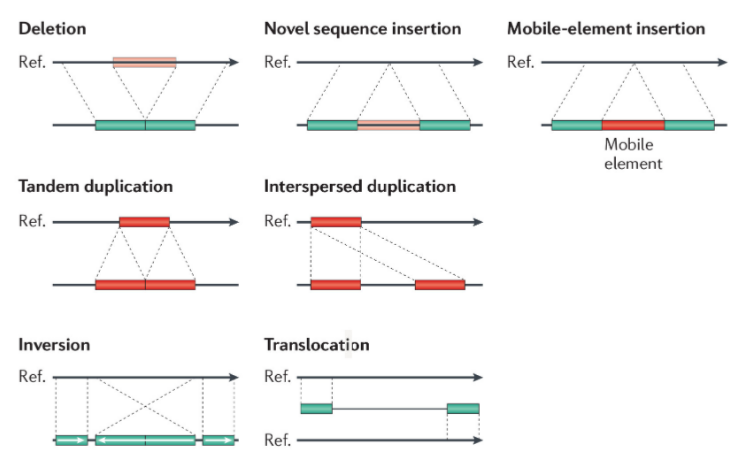
\includegraphics[width = 0.7\textwidth]{figs/types-sv.png}
\caption{Distintos tipos de variación estructural.}
\end{figure}

Varios mecanismos mutacionales pueden conducir a la generación de SV. Estos pueden ocurrir tanto meiótica como mitóticamente.
\begin{itemize}
\item Error en la recombinación
\item Errores en la reparación de ADN 
\item Errores en la replicación
\end{itemize}
Cada uno de estos métodos generaría una firma molecular particular en y alrededor de los puntos de rotura del SV.

\section{Detección de variantes estructurales}
Los tipos de variantes estructurales más estudiados son los que implican cambios en el número de copias de determinados fragmentos de material genético, ya que son más fáciles de detectar con las tecnologías actuales. Estos eventos se denominan colectivamente «variación del número de copias» (CNV). La detección de otros variantes desde NGS depende de la complejidad de los algoritmos: profundidad de lectura (o profundidad de cobertura), lectura pair-end, split read, ensamblaje de novo. 

\begin{figure}[h!]
\centering
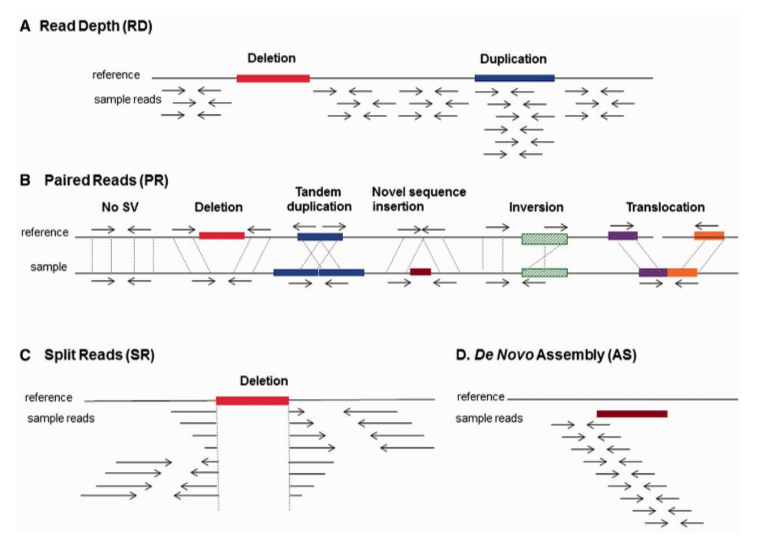
\includegraphics[width = 0.7\textwidth]{figs/sv-detection-methods.png}
\caption{Representación visual de los distintos métodos de detección de variantes estructurales.}
\end{figure}

El uso de lecturas pequeñas es especialmente difícil cuando se secuencian áreas que pueden repetirse a lo largo del genoma. Lecturas largas pueden resolver regiones complejas al anclarse en regiones normales. 

\section{Detección de CNV}
Como ya se ha mencionado, la variación estructural relacionada con los cambios en el número de copias de las regiones genómicas es la más fácil de caracterizar con las tecnologías actuales.
Existen dos técnicas principales actualmente en uso: la hibridación genómica comparativa (CGH) y la detección de CNV basada en secuenciación (CNV-seq).

\subsection{Hibridación genómica comparativa (CGH)}
Se coge una secuencia referencia y una muestra, marcándolas con fluorescentes distintos. Se hibrida, y dependiendo del color de la muestra resultante, se puede estimar la abundancia relativa. 

\begin{figure}[h!]
\centering
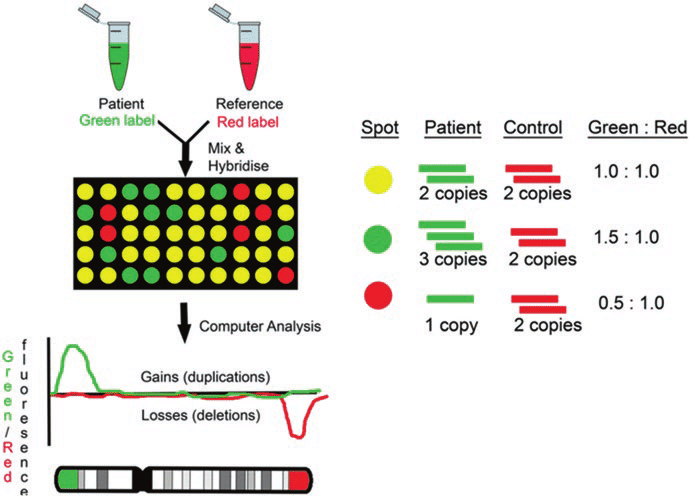
\includegraphics[width = 0.7\textwidth]{figs/Comparative-genome-hybridization-CGH-microarray-Karampetsou-et-al-2014.png}
\end{figure}

\subsection{CNV-seq}
El análisis de CNV basado en la secuenciación se basa en la detección de regiones del genoma con más (ganancia) o menos (pérdida) lecturas de lo esperado.
Puede realizarse mediante secuenciación del exoma completo (WES) o del genoma completo (WGS).
La llamada WES requiere una secuenciación muy profunda (100x), mientras que la WGS ha demostrado funcionar con una cobertura tan baja como 0,1x.
Esto se debe a que disponer del genoma completo nos permite crear una base estadística de lo que es «normal». Esto no es posible con sólo el 1\% del genoma (WES).

\begin{figure}[h!]
\centering
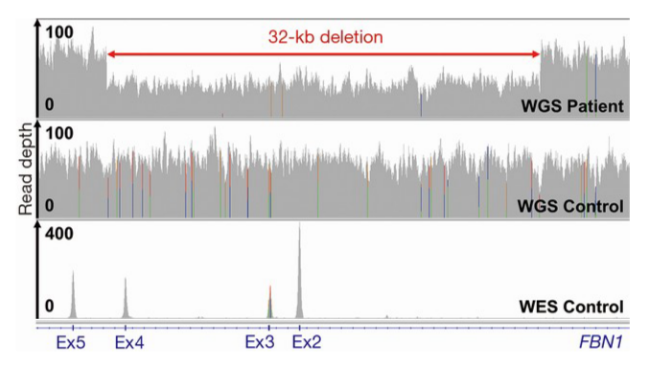
\includegraphics[width = 0.7\textwidth]{figs/cnv-calling-wgs.png}
\end{figure}

\subsection{CGH vs CNV-seq}
La CGH se considera el estándar dorado. Esto se debe a que para CNV-seq hay que hacer algunas suposiciones que harán que los diferentes métodos de análisis produzcan resultados potencialmente diferentes. Un ejemplo de la concordancia entre diferentes herramientas CNV-seq:

\begin{figure}[h!]
\centering
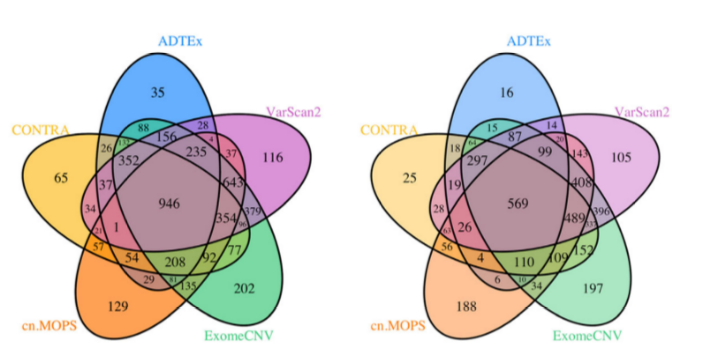
\includegraphics[width = 0.7\textwidth]{figs/cgh-vs-cnvseq.png}
\end{figure}

\subsection{Comprensión de la salida típica de CNV-seq}
Un gráfico típico de CNV sería como el siguiente:

\begin{figure}[h!]
\centering
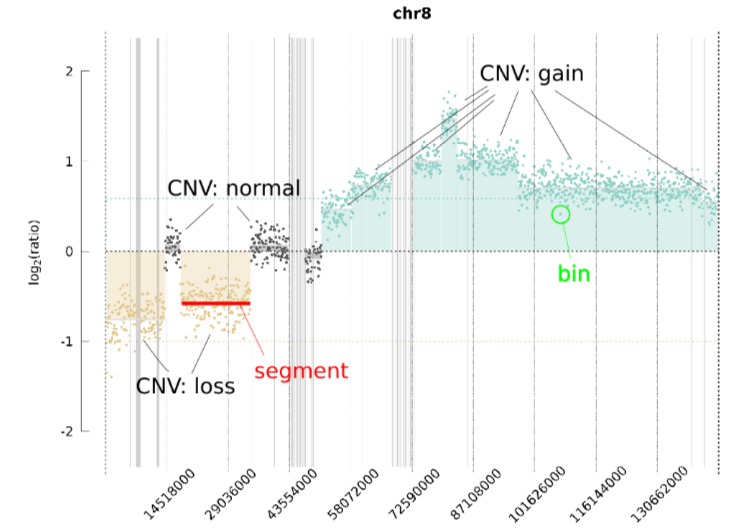
\includegraphics[width = 0.7\textwidth]{figs/cnv-plot.png}
\end{figure}
Los fragmentos grises son regiones sin resolver durante el ensamblado. 

El primer paso para realizar la llamada CNV es \textbf{dividir el genoma en intervalos no solapados} que cubren un determinado número de bases (por ejemplo, 50.000). Cada bin agrupa todas las lecturas que caen dentro de su área. Cuanto más pequeño sea el bin, mayor será la resolución y el detalle de los eventos CNV detectables.
El tamaño del bin (es decir, la resolución) depende de la profundidad de secuenciación, la ploidía del genoma y, en muestras de cáncer, la pureza del tumor, entre otros factores.
Cada bin se caracteriza por una relación log2, que representa la relación entre las lecturas observadas y las lecturas esperadas y el zscore para indicar su posición con respecto a la media.

El segundo paso es la \textbf{segmentación}: agrupar bins que parece que pertenecen al mismo segmento. Igual que los bins, se almacena en una tabla el ratio y el zscore. 

El paso final es la \textbf{llamada de aberraciones}, donde se asigna a los segmentos una probabilidad de ser un evento CNV verdadero mediante el zscore. La aberración es una etiqueta de eventos estadísticamente significativos. Son un subset de los segmentos que cuenta con una columna adicional que especifica si su tipo es una ganancia o una pérdida. Se utilizan colores para visualizarlo: el verde para ganancias y naranja para pérdidas. 

\section{Práctica - variantes estructurales}
En esta sección analizaremos algunas muestras utilizando WisecondorX para realizar llamadas CNV.
Comenzaremos con los resultados de los alineamientos con el genoma humano en formato BAM.
El resultado que obtengamos del llamador de CNV debería ayudarnos a arrojar algo de luz sobre la situación estructural de las muestras analizadas.

Al igual  que en las prácticas anteriores, primero se crea un entorno de conda con el software que se va a utilizar. Con el script de configuración se descargaron 10 ficheros de muestras control que se espera que no contengan eventos de CNV y dos muestras que queremos comparar. 

Ahora vamos a indexar nuestros archivos BAM, lo que es necesario para la mayoría de los análisis que hacen el acceso aleatorio de las alineaciones.
\begin{lstlisting}[language=bash]
parallel -j $(nproc) samtools index {} ::: data/*.bam
\end{lstlisting}

Ahora tenemos que convertir nuestros archivos BAM en archivos npz (archivos numpy arrays comprimidos), que es el formato que WisecondorX utilizará posteriormente.
\begin{lstlisting}[language=bash]
mkdir -p out/npz
time parallel -j $(nproc) WisecondorX convert {} out/npz/{/.}.npz ::: data/*.bam
#Alternativa: ls data/*.bam | parallel -j $(nproc) WisecondorX convert {} out/npz/{/.}.npz
\end{lstlisting}

A continuación creamos la referencia con la que comparar nuestras muestras control.
\begin{lstlisting}[language=bash]
mkdir -p out/ref
WisecondorX newref out/npz/control*.npz out/ref/reference.npz \
    --yfrac 1 --cpus $(nproc)
\end{lstlisting}

Finalmente, obtenemos las predicciones de nuestras muestras.
\begin{lstlisting}[language=bash]
mkdir -p out/predictions
parallel WisecondorX predict {} out/ref/reference.npz out/predictions/{/.} --bed --plot ::: out/npz/sample*.npz
\end{lstlisting}

En este punto, se han generado algunos plots en PNG. Tras abrirlos, vemos que los gráficos de sample1 son planos. Las nubes de puntos están extremadamente dispersas y no se puede determinar nada. En el caso de sample2, las nubes de puntos, pese a seguir siendo muy dispersas, sí permite ver algunos eventos de ganancia y pérdida. 

También podemos crear gráficos CNV basados en los resultados de WisecondorX. Para ello utilizaremos un script python personalizado.
Este script generará gráficos para los cromosomas 8, 10 y 13 de nuestras muestras.
\begin{lstlisting}[language=bash]
mkdir -p scripts
wget -P scripts https://gitlab.com/bioinfo-lessons/intro-sv/-/raw/master/scripts/plots.py
python scripts/plots.py
\end{lstlisting}

Este script genera los mismos gráficos, pero marcando algunos oncogenes como MYC. En los gráficos de los cromosomas 8, 10 y 13, se ve cómo sample2 tiene una pérdida de los supresores tumorales BRCA2 y RB1.

Ahora vamos a visualizar la salida de WisecondorX en IGV. Para ello, debemos eliminar la cabecera de los ficheros bed.
\begin{lstlisting}[language=bash]
for f in out/predictions/*.bed; do grep -v "start" $f > $(dirname $f)/$(basename $f .bed).igv.bed; done;
\end{lstlisting}
A continuación cargamos los segmentos y las aberraciones en IGV. Haciendo click derecho en cada una de las cuatro pistas, se puede seleccionar el modo de vista ampliada. 

Como conclusión de la práctica, hemos observado algunas pérdidas en genes supresores de tumores (BRCA2, RB1) y ganancias en un oncogén (Myc).
Esto indicaría que nuestra muestra afectada (sample2) procede de un paciente que padece algún tipo de cáncer, que es de hecho el origen de la muestra.

%18/11 - Dido Carrero
\part{Variantes genómicas: técnicas, llamada de variantes y anotación}
\chapter{Introducción a las variantes germinales}
\section{Análisis genómico}
El análisis genómico incluye varios pasos: primero, la extracción de muestras y la preparación de las librerías; luego, la secuenciación, el control de calidad de los archivos FastQ (donde se descartan las lecturas con errores, ya que una mayor refinación del pipeline implica un control de calidad más estricto); el alineamiento de las lecturas; la identificación o llamada de variantes (SNP, INDEL, CNV, SV); la anotación de los archivos VCF; la visualización de las variantes candidatas y, finalmente, los pasos de priorización y filtrado.

En general, en un análisis de genoma, pueden encontrarse muchas variantes en comparación con el genoma de referencia, por lo que es necesario aplicar filtros para identificar aquellas que sean realmente relevantes a nivel clínico. La validación final se realiza en el laboratorio mediante PCR.

Las variantes germinales se originan en la línea germinal, es decir, en los gametos, lo que las hace heredables y presentes en todo el organismo. En cambio, las variantes somáticas ocurren en células que no pertenecen a los gametos, son mutaciones adquiridas durante la vida y afectan solo a un linaje celular específico.

En la práctica, ya sea que se realice un análisis somático o germinal, se extraen muestras tanto del tejido tumoral como del tejido sano. Si se sospecha de una enfermedad genética germinal, también se debe extraer una muestra de un tejido germinal.

La frecuencia alélica es la proporción de moléculas de ADN en la muestra que contienen una mutación específica. Se calcula mediante la siguiente fórmula:
$$VAF = \frac{sequence.reads.with.a.DNA.variant}{overall.coverage.at.that.locus}$$
Este número es clave para diferenciar una variante somática de una germinal. En un organismo diploide, un locus heterocigoto debería mostrar un VAF cercano a 0,5, un locus homocigoto tendrá un VAF de 1 y un locus de referencia tendrá un VAF de 0. Las variantes somáticas presentan una frecuencia alélica muy variable, mientras que las variantes germinales suelen tener valores de VAF de 0, 0,5 o 1, dependiendo de si están presentes en uno, ambos o ninguno de los alelos.

\subsection{GATK}
GATK es un conjunto de herramientas desarrollado por el Broad Institute para el análisis de variantes genómicas. A partir de archivos BAM, estas herramientas permiten realizar un análisis completo de variantes. El paquete incluye buenas prácticas y un flujo de trabajo (workflow) que varía dependiendo de si se analizan variantes germinales o somáticas.

\begin{figure}[h!]
\centering
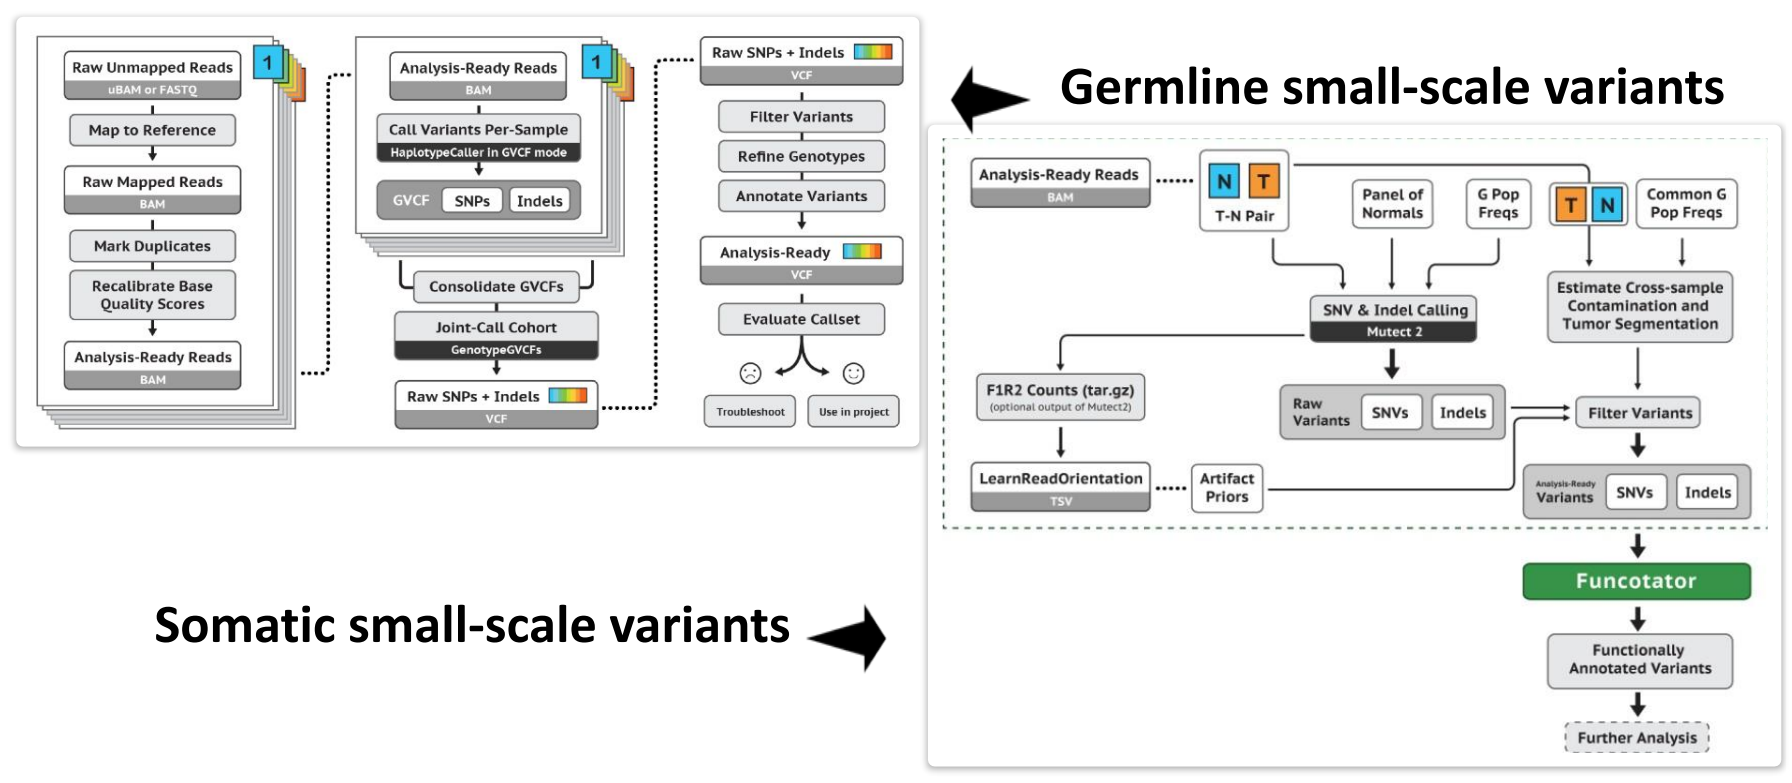
\includegraphics[width = 0.8\textwidth]{figs/gatk-pipelines.png}
\end{figure}

HaplotypeCaller es una herramienta utilizada para la llamada de variantes, basándose en el cálculo de la probabilidad de los genotipos. Utiliza un archivo BAM como entrada y produce un archivo de salida en formato VCF o GVCF con los genotipos 1/1, 0/1 y 0/0. Este archivo VCF debe ser filtrado mediante recalibración de bases (una práctica recomendada) o mediante hard-filtering. Si el archivo de salida es un GVCF, será necesario realizar un paso intermedio antes de aplicar el filtro y continuar con el análisis posterior. Además, con la opción -ploidy, se puede especificar la ploidía del organismo.

El comando básico para la herramienta es:
\begin{lstlisting}[language = bash]
gatk HaplotypeCaller \
	-R reference.fasta \
	-I preprocessed_reads.bam \
	-O germline_variants.vcf
\end{lstlisting}

MuTect2 es una herramienta diseñada para la llamada de variantes somáticas. Permite detectar SNVs e INDELs, con frecuencias alélicas variables, y es capaz de diferenciar entre variantes somáticas y germinales. MuTect2 ofrece varios modos: tumor con normal emparejado, solo tumor o modo mitocondrial.

\section{Práctica: análisis de datos}
Vamos a recibir los datos de cáncer de mama. Se ha secuenciado todo el exoma con Illumina. Primero creamos el entorno conda \texttt{OVCA\_case}. 
\begin{lstlisting}[language=bash]
conda create -n OVCA_case
conda activate OVCA_case
conda install bioconda::gatk4
conda install bioconda::samtools
\end{lstlisting}

Con los datos descargados, utilizamos la herramienta HaplotypeCaller. Lo primero que debemos hacer es realizar los índices de la referencia y del fichero bam:
\begin{lstlisting}[language=bash]
samtools dict  REFERENCE/hg19_chr17.fa -o  REFERENCE/hg19_chr17.dict
samtools faidx REFERENCE/hg19_chr17.fa
samtools index bams/normal_refined.bam
\end{lstlisting}

A continuación utilizamos la herramienta:
\begin{lstlisting}[language=bash]
gatk HaplotypeCaller -R REFERENCE/hg19_chr17.fa -I bams/normal_refined.bam -O out/normal_refined_out.vcf
\end{lstlisting}

El fichero resultante empieza con una cabecera con dos almohadillas y el cromosoma de referencia. Se muestra la información acerca de la generación del fichero y los filtros. Con una almohadilla se muestra el significado de cada columna: cromosoma en el que está la variante, posición genómica, ID, alelo de referencia, alelo alternativo con la mutación encontrada, score de calidad, filtros, información adicional con la anotación, formato del siguiente campo y normal. Dentro del formato, se distinguen: GT indica el genotipo, AD el número de lecturas que soporta la variante (en formato referencia,variante) y DP el total de lecturas.

El siguiente paso es la recalibración de variantes. Muchas veces, la calidad de las variantes que aparece de manera directa (columna QUAL) se debe recalibrar. Este modelo puntúa las calidades de las variantes y filtrar aquellas que no pasen los filtros. Se comprueba que una variante sea efectivamente verdadera. Para ello, se da un archivo de referencia de variantes y se estima si la variante es un artefacto de la secuenciación o una variante de verdad. El resultado es VQSLOD, que se añade al campo de información. Esto en general se realiza para SNPs e INDELs por separado debido a que las bases de datos de variantes son diferentes. 

El paso siguiente es aplicar los filtros VQSR. En la columna FILTER anota si la variante pasa filtros o no, pero no descarta aquellos que no pasen los filtros; si se quiere eso se debe especificar.
\begin{lstlisting}[language=bash]
tabix -p vcf Annotations/dbsnp_138.hg19_chr17.vcf.gz

gatk VariantRecalibrator -R REFERENCE/hg19_chr17.fa -V out/normal_refined_out.vcf
--resource:dbsnp,known=true,training=true,truth=true,prior=15.0
Annotations/dbsnp_138.hg19_chr17.vcf.gz -an QD -an ReadPosRankSum -an FS -an SOR -mode BOTH -O out/output_normal_refined.recal --tranches-file out/output_normal_refined.tranches

gatk ApplyVQSR -R REFERENCE/hg19_chr17.fa -V out/normal_refined_out.vcf -O out/output_normal_refined.recalibrated --truth-sensitivity-filter-level 99.0 --tranches-file out/output_normal_refined.tranches --recal-file out/output_normal_refined.recal -mode BOTH
\end{lstlisting}

El último paso es el filtrado de las variantes. 
\begin{lstlisting}[language=bash]
awk -F '\t' '{if ($0 ~ /#/ || $7 == "PASS") print}' out/output_normal_refined.recalibrated > out/output_normal_refined.onlypass

#Contar el número de líneas resultantes
grep "^chr17" out/output_normal_refined.onlypass | wc -l
\end{lstlisting}

%21/11 - Dido
\chapter{Introducción a las variantes somáticas}
\section{Control de calidad y refinamiento de alineamientos}
\subsection{Control de calidad}
Los controles de calidad se suelen hacer en varios puntos de todo el proceso. Hay varios puntos clave, y después de cada uno de ellos se realiza el control de calidad. El primero y más importante parte de los archivos FastQ de secuenciación, ya que si éstos están mal, el resto del análisis carece de sentido.

Se utiliza el programa FastQC que da un informe en HTML con varias estadísticas de los archivos. Hay otros programas que se pueden utilizar, como samtools, que indica si hay secuencias duplicadas y otras estadísticas. MultiQC combina varias herramientas para sacar un informe completo.

En los controles de calidad, se mira si hay un número de lecturas dentro del rango esperado, si las bases tienen una buena calidad mediante el Phred score, y si hay contaminación en las muestras. Una secuencia que aparezca repetidamente puede ser muy repetitiva en el genoma que se secuencie o una contaminación.

FastQC permite visualizar la calidad por base por secuencia, el contenido GC y secuencias sobrerrepresentadas entre otras métricas, pero esas son las que habitualmente están mal. En cuanto a la evaluación de la calidad por base, se ve la distribución de los scores en las lecturas. En secuenciación de Illumina, es habitual que al final de las lecturas la calidad decaiga un poco, pero debería seguir en un rango elevado. Si la calidad decae mucho, se trata de un error en la secuenciación. En los scores por secuencia, se espera que la mayoría de las secuencias tengan una puntuación muy alta. Si hay varias secuencias con una calidad baja, eso indica que algo está mal, pero es difícil indicar la causa (problema del secuenciador, purificación de las muestras, contaminación, librería, etc). La distribución esperada del contenido en GC debería seguir una distribución normal, aunque hay veces que se puede desviar un poco.

\begin{lstlisting}[language=bash]
conda install bioconda::fastqc
fastqc -o out/ Raw_data/*.fastq
\end{lstlisting}

El resultado es un fichero html y zip por cada FastQ. En cuanto a Normal R1, el contenido GC muestra un mensaje de error. Hay un pico muy grande alrededor del 60\%, cuando en humanos debería rondar el 50\%. Además, hay varias lecturas con un contenido GC bajo, sobre el 35\%. Como estos resultados son malos, se puede valorar descartarlos y repetir la secuenciación, pero en laboratorios pequeños puede ser un problema. Además, tenemos una secuencia sobrerrepresentada de N, que no nos preocupa porque se va a descargar. Todas las demás métricas han salido bien. En Normal R2, las secuencias sobrerrepresentadas dan error, pero sigue siendo una secuencia de todo N, por lo que se le puede dar poca importancia. El contenido GC también da error. En cuanto a las muestras de tumor, son muy similares: tienen un contenido GC más bajo y tiene una secuencia de N sobrerrepresentada. 
Hay que tener en cuenta que estamos trabajando solo con el cromosoma 17, pero que la distribución esperada está calculada sobre todo el genoma. Por tanto, si ese cromosoma tiene muchas secuencias repetitivas en AT, ya de por sí habrá un sesgo en la comparación con la distribución esperada. 

\subsection{Alineamiento}
En cuanto al alineamiento, se utiliza BWA. Se puede utilizar la siguiente chuleta para la indexación en base al fichero que se tenga:
\begin{lstlisting}[language=bash]
#Fasta
bwa index reference.fasta
samtools dict reference.fasta -o reference.dict
samtools faidx reference.fasta

#BAM
samtools index bam.file

#VCF
tabix -p vcf vcf.file
\end{lstlisting}

El siguiente paso es la alineación.
\begin{lstlisting}[language=bash]
bwa mem -R '@RG\tID:OVCA\tSM:Normal' REFRENCE/hg19_chr17.fa Raw_data/WEx_Normal_R1.fastq Raw_data/WEx_Normal_R2.fastq > alignment/normal.sam
bwa mem -R '@RG\tID:OVCA\tSM:Tumour' REFRENCE/hg19_chr17.fa Raw_data/WEx_Tumour_R1.fastq Raw_data/WEx_Tumour_R2.fastq > alignment/tumour.sam
\end{lstlisting}

Se puede utilizar \texttt{samtools flagstat normal.sam} para ver unas estadísticas como alineamientos mapeados, primarios, secundarios, duplicados, etc. 

\subsection{Refinamiento del alineamiento}
En este paso, queremos convertir los SAM en BAM para que los ficheros estén comprimidos y binarizados. Además, BWA a veces omite alguna información en los ficheros SAM que queremos rellenar.
\begin{lstlisting}[language=bash]
samtools fixmate -O bam alignment/normal.sam alignment/normal_fixmate.bam
samtools fixmate -O bam alignment/tumour.sam alignment/tumour_fixmate.bam
\end{lstlisting}

Los duplicados vienen de la amplificación por PCR durante la preparación de la librería. Un error al principio de la PCR se propaga. Los duplicados en secuenciación híbrida no aportan nada al análisis posterior, pudiendo dar lugar a falsos positivos y redundancia. Por ello, lo mejor es descartar estas duplicaciones. Además, para la llamada de variantes es necesario que el alineamiento esté ordenado por posición genómica, y aprovechamos para indexar el BAM.
\begin{lstlisting}[language=bash]
samtools sort -O bam -o alignment/normal_sorted.bam alignment/normal_fixmate.bam
samtools sort -O bam -o alignment/tumour_sorted.bam alignment/tumour_fixmate.bam

samtools rmdup -S alignment/normal_sorted.bam alignment/normal_refined.bam
samtools rmdup -S alignment/tumour_sorted.bam alignment/tumour_refined.bam

samtools index alignment/normal_refined.bam
samtools index alignment/tumour_refined.bam
\end{lstlisting}

Con esto hemos creado los bams que utilizamos en la parte anterior de las variantes germinales. Se pueden eliminar los ficheros intermedios de ficheros sam, fixmate y sorted, dejando los bam refinados.

\section{Recalibración de la calidad de base}
Cada posición de la secuencia tiene su calidad de base. Las diferentes tecnologías NGS tienen sus sesgos dependiendo del contexto, por lo que es importante hacer la recalibración para corregir empíricamente esos sesgos. La recalibración de bases no es lo mismo que la recalibración de variantes (eso viene después con los VCF).

La recalibración de bases consta de dos pasos. Primero, BaseRecalibrator parsea las lecturas y crea una tabla en la que se asigna a cada lectura el ciclo durante el que se leyó la base, su puntuación y la puntuación de las bases que van antes y después. EL modelo computa cuántas veces hay un cambio en la referencia según dbSNP, excluyendo los loci de alta variabilidad. Después, la herramienta ApplyBQSR parsea las lecturas y, utilizando la matriz de antes, recalibra las puntuaciones. Así, las calidades son más similares a las puntuaciones empíricas, pudiendo utilizarse para el variant calling.

\section{Llamada de variantes somáticas}
Las variantes son cambios permanentes en el ADN de un organismo que pueden deberse a errores durante la replicación, durante la recombinación durante la formación de gametos y por factores externos como radiación, viruses, transposones, rayos ultravioleta, etc. El genoma entre humanos es idéntico en un 99,9\%. El 0,1\% restante es la fuente de variabilidad, permitiendo los mecanismos de evolución, las diferencias fenotípicas entre individuos y en la respuesta a enfermedades y fármacos. 

\begin{figure}[htbp]
\centering
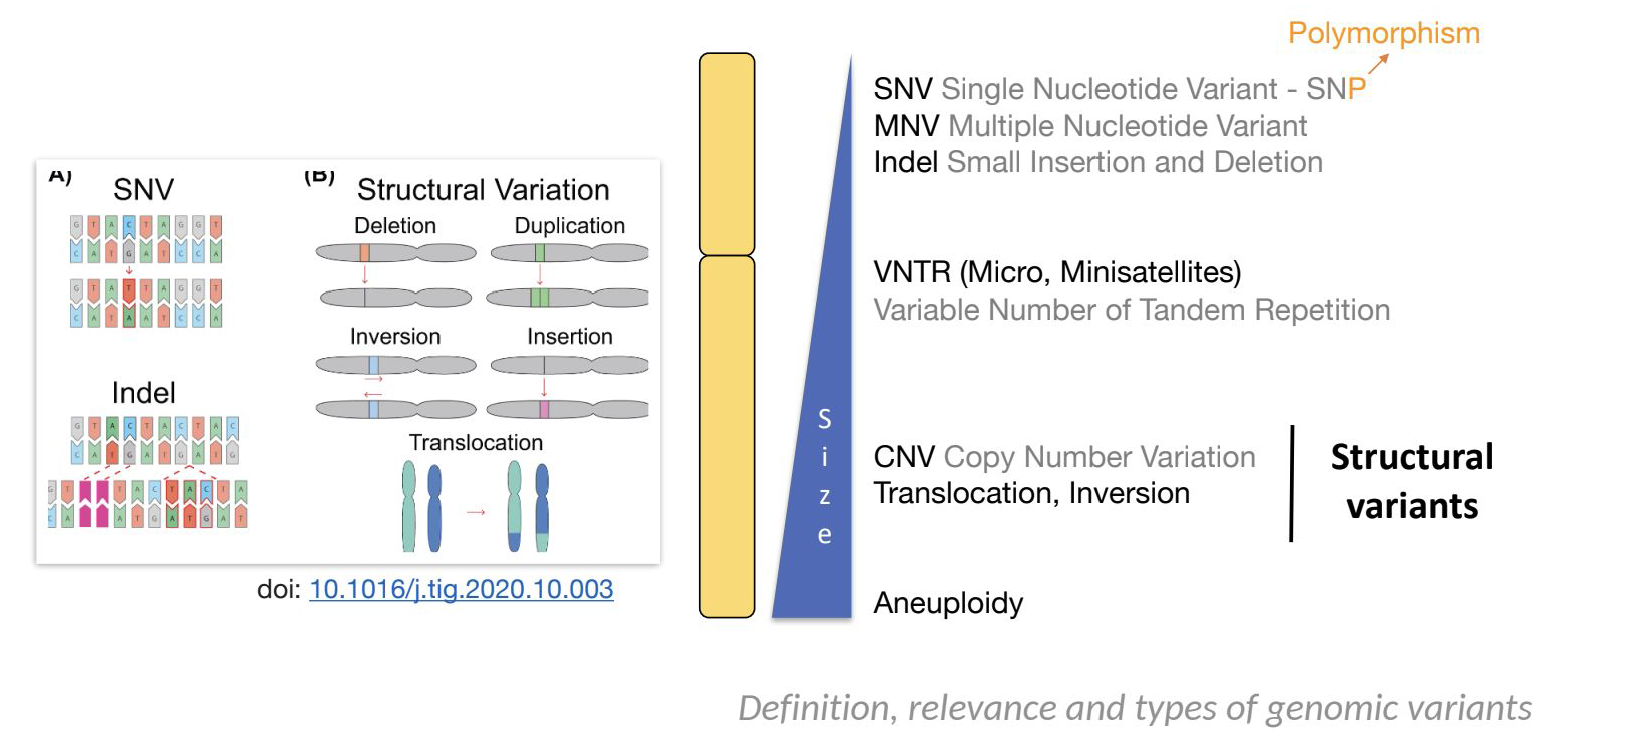
\includegraphics[width = \textwidth]{figs/variants-size.png}
\end{figure}

En función de la posición de la secuencia, puede haber variantes intergénicas (entre genes) en secuencias reguladoras o upstream o downstream de algún gen en concreto. Dentro de genes, puede haber variantes en las regiones UTR, en los exones, en los intrones o en regiones de splicing. 

Para realizar la llamada de variantes, se utiliza MuTect2. Es similar a GATK, pero permitiendo mayor variabilidad de frecuencia alélica (no solo 0, 0,5 y 1 como GATK), además de evitar las variantes germinales. Hay distintos modos: tumor con tejido normal (este es el óptimo), solo tumor y mitocondrial. Se crea un panel de normales para poder inferir qué mutaciones son exclusivamente somáticas. 
\begin{lstlisting}[language=bash]
#Modo Tumor-only 
gatk Mutect2 -R REFERENCE/hg19_chr17.fa -I alignment/tumour_refined.bam -O tumour_only_somatic.vcf

#Modo tumor with matched normal
gatk Mutect2 -R REFERENCE/hg19_chr17.fa -I alignmetn/tumour_refined.bam -I alignment/normal_refined.bam -normal Normal -O out/tumour_matched_somatic.vcf
\end{lstlisting}
 
Después del filtrado, obtenemos las siguientes variantes somáticas:
\begin{lstlisting}[language=bash]
grep "^chr17" out/tumour_matched_somatic.vcf | wc -l #193
grep "^chr17" out/tumour_only_somatic.vcf | wc -l #461
\end{lstlisting}
Cuando solo se mide el tumor, el número es casi el doble. Al dar el normal, el algoritmo sabe qué variantes son germinales por estar ya presentes en el tejido y los descarta. Al medir solo el tumor, algunas variantes germinales se excluyen, pero otras se cuelan, por lo que el número de variantes es mayor. 

Las frecuencias alélicas vienen en la columna FORMAT bajo AF. Estas frecuencias van del 0 al 1 en todo el rango. En las variantes germinales, esta información aparece en INFO y es de 0, 0,5 o 1. 

El fichero de solo tumor, tiene más variantes porque no puede excluir todas las variantes germinales. No obstante, el número de mutaciones sigue siendo mayor que la suma de tumor matched y las mutaciones germinales calculadas en la parte anterior. Esto se debe a que, al calcular las variantes germinales, el algoritmo solo se queda con aquellas que tengan una frecuencia alélica de 0,5 o de 1, no con todo el rango como el que detecta tumor only. Por ejemplo, por contaminación, tumor only puede detectar una variante germinal que no esté al 0,5 o 1 y que, por tanto, esté excluida del análisis de variantes germinales. El fichero de tumor only siempre va a  tener más variantes.

%25/11 - Dido
\chapter{Anotación de variantes}
La anotación de variantes consiste en enriquecer los archivos VCF con información adicional útil para su priorización. Esta información proviene tanto de bases de datos como de cálculos basados en la posición genómica de las variantes.

Dado el gran número de variantes en un archivo VCF, es impráctico evaluarlas manualmente. Como no todas tienen impacto relevante en el fenotipo de estudio, se aplican filtros para reducir el conjunto a las variantes potencialmente relevantes. Esto incluye descartar variantes comunes, benignas o de significancia incierta (VUS, variants of unknown significance).

En una anotación estándar, se incluye información sobre:
\begin{itemize}
\item Tipo de variante (SNV, indel, etc.)
\item Localización genómica
\item Consecuencias en la secuencia
\item Predicción del impacto funcional
\item Frecuencia poblacional
\item Asociación con patologías conocidas
\end{itemize}

\section{Nomenclatura de variantes}
Las variantes se identifican por el cromosoma, la coordenada genómica, el alelo de referencia y el alelo alternativo. Existen dos genomas de referencia principales: hg19 y hg38. El más reciente, hg38, es el recomendado para investigaciones actuales. Para convertir coordenadas entre estas referencias, se puede utilizar la herramienta Liftover disponible en UCSC.

El impacto en el ADN codificante y en la proteína se describe según la nomenclatura HGVS:
\begin{itemize}
\item g. genomic reference sequence
\item c. coding DNA reference sequence
\item m. mitochondrial DNA reference sequence
\item n. non-coding DNA reference sequence
\item r. RNA reference sequence (transcript)
\item p. protein reference sequence
\end{itemize}

Para asegurar la uniformidad, se recomienda seguir las \href{https://hgvs-nomenclature.org/stable/recommendations/general/}{guías estandarizadas para la nomenclatura HGVS}.

Las mutaciones pueden tener efectos diferentes en los transcritos de un mismo gen debido al splicing alternativo. Algunas enfermedades surgen por mutaciones que afectan transcritos minoritarios mientras que el principal permanece intacto. Para gestionar esta complejidad, se usan identificadores únicos, como los de Ensembl:
\begin{itemize}
\item Gene Identifiers: ENSG 
\item Transcript Identifiers: ENST
\end{itemize}

Además, las bases de datos como \href{https://www.genecards.org/}{GeneCards} o \href{https://www.genenames.org/}{GeneNames} ayudan a identificar el nombre oficial del gen, ya que un mismo gen puede tener varios nombres comunes.

Ensembl proporciona información detallada sobre cada gen, sus transcritos y biotipos, junto con equivalencias entre diferentes bases de datos. Por ejemplo:
\begin{itemize}
\item RefSeq incluye principalmente el transcrito principal
\item MANE es una anotación colaborativa que indica el transcrito principal
\end{itemize}

Para proteínas, la base de datos por referencia es \href{https://www.uniprot.org/}{Uniprot},  que incluye información sobre función, localización subcelular, relación con enfermedades y efectos de mutaciones.
Además, APPRIS (proyecto de Gencode) identifica transcritos principales y sus isoformas, categorizados como MANE, canonical o APPRIS principal.

\section{Consecuencias en la secuencia}
El impacto de una variante depende de su ubicación dentro del gen o región reguladora. Las consecuencias están codificadas y documentadas en \href{https://www.ensembl.org/info/genome/variation/prediction/predicted_data.html}{Ensembl}. 

\begin{figure}[htbp]
\centering
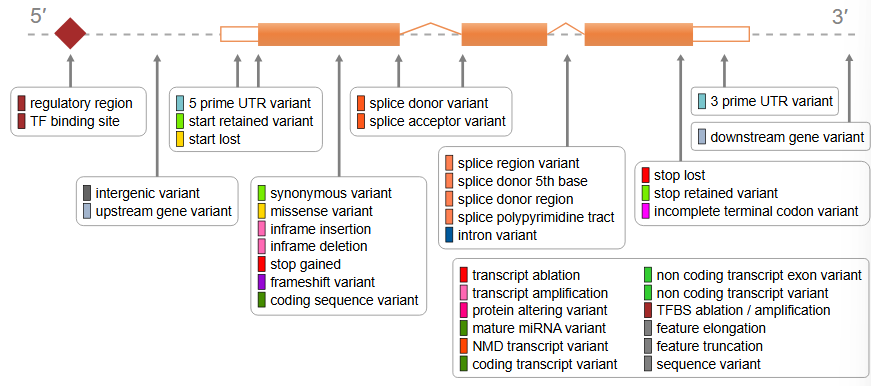
\includegraphics[width = \textwidth]{figs/consequences.png}
\end{figure}

\begin{itemize}
\item Mutaciones puntuales:
\begin{itemize}
\item Missense: cambian un aminoácido. Pueden ser conservativas o no conservativas en función de si mantienen la polaridad.
\item Nonsense: introducen un codón de parada
\item Silentes: no afectan al aminoácido
\end{itemize}
\item Mutaciones inframe: no alteran el marco de lectura
\item Mutaciones frameshift: cambian el marco de lectura, afectando significativamente la proteína.
\end{itemize}

Las consecuencias se clasifican según su impacto:
\begin{itemize}
\item Alto: frameshift, nonsense
\item Moderado: missense
\item Bajo: silentes
\item Modificador: sin efecto directo conocido
\end{itemize}

Esta clasificación facilita priorizar variantes según su potencial efecto dañino.

\section{Predicción del impacto funcional}
Existen numerosos algoritmos para predecir el impacto de variantes en la función y estructura de proteínas. Estos se agrupan en:
\begin{itemize}
\item Predictores para variantes missense
\item Predictores para variantes que afectan el splicing
\item Predictores basados en la conservación evolutiva
\end{itemize}

\subsection{Predictores para variantes missense}
El hecho de que haya tantos predictores hace que haya varias escalas para predecir el impacto de un cambio. Cada software tiene su escala y sus criterios para ver si una variante es benigna o no. Por ello, se realiza la anotación con varios y se busca el consenso entre ellos. Algunos predictores son:
\begin{itemize}
\item \textbf{Sift:} evalúa el efecto funcional basándose en homología y propiedades de aminoácidos. Score: 0-1 (más bajo = mayor impacto); < 0,05 deleterious
\item \textbf{PolyPhen:} basado en estructura y función proteica. Score: 0-1 (más alto = mayor impacto); benigno < $\sim$ 0,435 < dañino
\item \textbf{Revel:}  integra 13 herramientas, incluidas SIFT y PolyPhen, para una predicción más robusta.
\item \textbf{ClinPred:} utiliza machine learning para identificar variantes relevantes en enfermedades, incorporando frecuencias alélicas de gnomAD.
\item \textbf{AlphaMissense:} se trata de una adaptación de AlphaFold ajustada a bases de datos de frecuencias de poblaciones de variantes humanas y primates para predecir la patogenicidad de variantes sin sentido combinando el contexto estructural y la conservación evolutiva. Genera predicciones para todas las posibles sustituciones de aminoácidos en humanos y clasificación del 89\% de las variantes sin sentido como probablemente benignas o patógenas.
\end{itemize}

Como no hay consenso, a la hora de realizar la prioridad hay que tener en cuenta su score. Estos predictores tienen una precisión y especificidad moderada, por lo que se deben utilizar en conjunto y ver el consenso.

\subsection{Predictores para variantes de splicing}
En cuanto a los predictores de splicing, uno muy notable es \textbf{SpliceAI}. Se trata de una herramienta basada en deep-learning que identifica las variantes de splicing y predice el efecto. La puntuación delta de una variante oscila entre 0 y 1 y puede interpretarse como la probabilidad de que la variante altere el splicing. En el artículo se ofrece una caracterización detallada de los valores de corte de 0,2 (alta recuperación), 0,5 (recomendado) y 0,8 (alta precisión).

\section{Frecuencias poblacionales}
Las frecuencias poblacionales ayudan a filtrar variantes comunes. Si una variante aparece en más del 1\% de la población, se considera un polimorfismo y generalmente no se asocia a enfermedades graves. Estas variantes pueden causar diferencias desde el color de pelo a la respuesta frente a fármacos. Las bases de datos clave son:
\begin{itemize}
\item gnomAD: es la más completa, con datos de 807,162 individuos divididos entre exomas y genomas completos, y estratificados por población y sexo. También incluye una versión con individuos sanos. Las variantes se pueden buscar mediante las coordenadas de hg38.
\item Proyecto 1000 Genomas
\item dbSNP
\item CIBERER: servidor de variantes en la población española con 2.100 exomas. Permite obtener información mucho más concreta de la población
\end{itemize}

\section{Asociación con enfermedades}
Muchas bases de datos incluyen información aportada por mutaciones in silico o in vivo que guardan relación con el desarrollo de una enfermedad. Algunas de ellas son de pago (como HGMD), pero hay otras buenas de libre acceso.
\begin{itemize}
\item \textbf{ClinVar}: recoge una serie de mutaciones (principalmente pequeñas SNV e indels, aunque hay algunas CNV), dando información sobre la clasificación clínica de la variante (benigna, probablemente benigna, patogénica, probablemente patogénica, respuesta a fármacos, factor protector para una condición, factor de riesgo, etc.), la enfermedad que causa y estatus de revisión. La mayor parte de las variantes son de significado incierto.
\item \textbf{OMIM}: es una base de datos de genes humanos y trastornos y rasgos genéticos con un enfoque particular en la relación gen-fenotipo. La búsqueda se realiza por enfermedad para ver todas las variantes asociadas a la misma.
\item \textbf{COSMIC}: es una base de datos en línea que recoge las mutaciones somáticas descubiertas en el cáncer humano. Recopila datos de publicaciones científicas y de estudios experimentales a gran escala.
\item \textbf{DisGeNET}
\end{itemize}

\section{Herramientas de anotación}
Las herramientas de anotación más comunes son:
\begin{itemize}
\item \textbf{Variant Effect Predictor (VEP):} se trata de una herramienta de Ensembl, siendo la más utilizada y completa. Proporciona anotaciones para los distintos tipos de alteraciones en las diferentes localizaciones genómicas. Tiene una versión en línea de comandos, pero también una \href{https://www.ensembl.org/info/docs/tools/vep/index.html}{versión web}. Permite incluir los identificadores de gen, versión del transcrito, UniProt y HGVS, además de muchos otros predictores e información. 
\item \textbf{ANNOVAR}
\item \textbf{Variant Effect}
\item \textbf{Predictor}
\item \textbf{VarAFT}
\item \textbf{SnpEff}
\end{itemize}

Utilizando VEP con los datos generados en la llamada de variantes somáticas con tejido normal pareado, los resultados son los siguientes (muchas columnas de la tabla están ocultas, como la puntuación de los distintos predictores):
\begin{figure}[htbp]
\centering
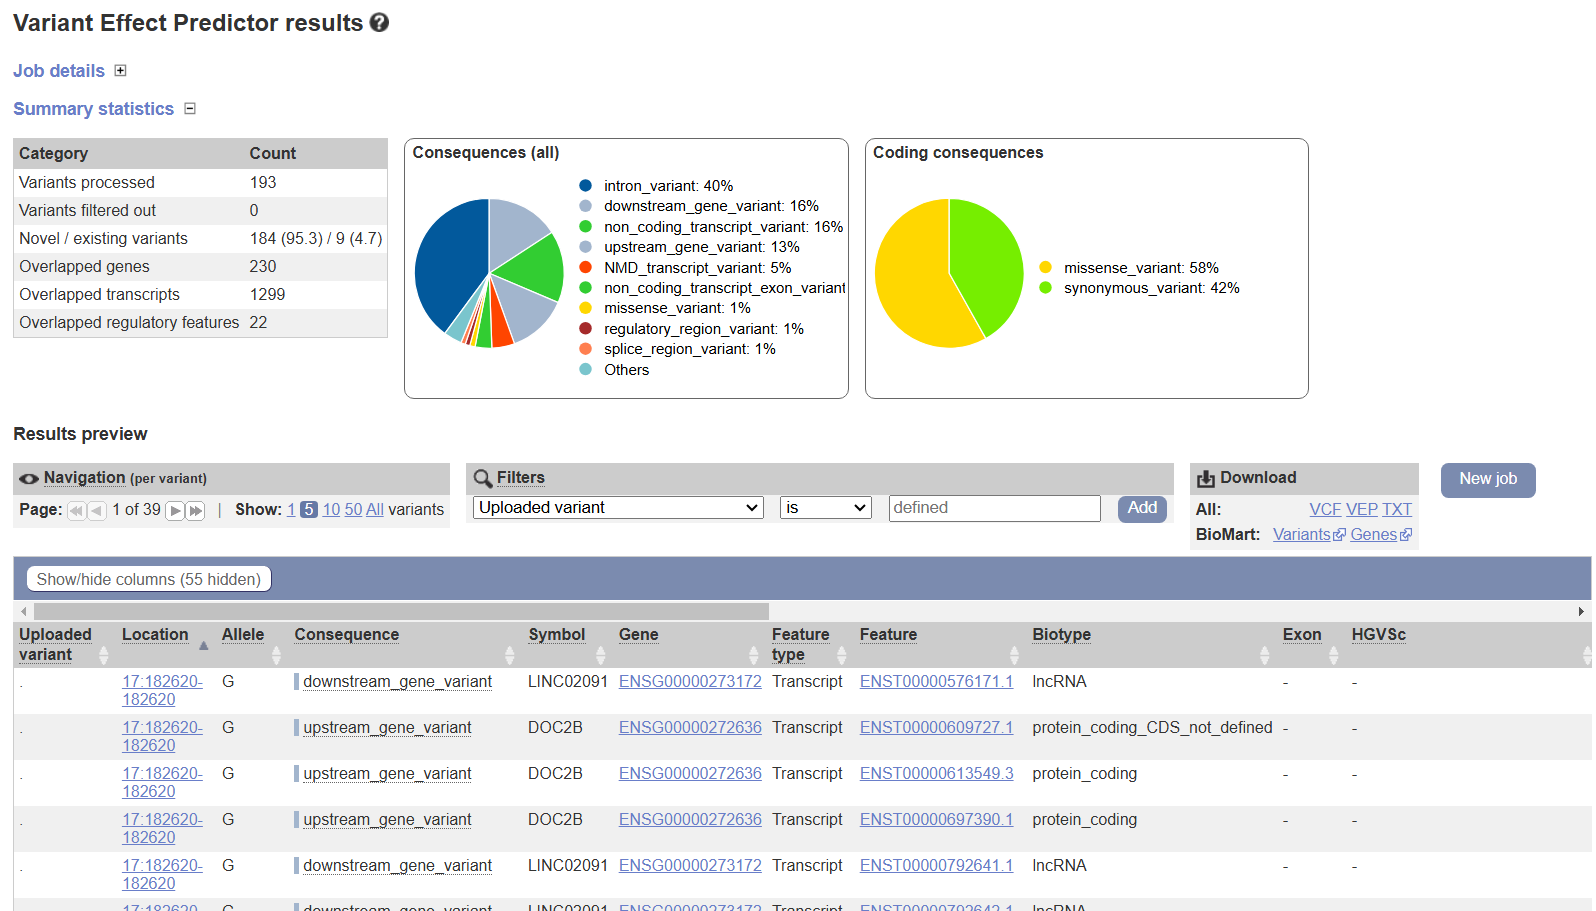
\includegraphics[width = \textwidth]{figs/vep-result.png}
\end{figure}

Para priorizar, se tendría en cuenta el score de AlphaMissense, SpliceAI, ClinPred, Revel, Sift y PolyPhen, buscando un consenso entre todos. Además, se puede buscar el identificador en ClinVar por si se hubiese recogido una asociación.

%26/11 - Dido
La priorización es un paso posterior, y en ocasiones nos podemos quedar en la descripción de lo que hay en las muestras sin profundizar cuál puede ser la mutación clave. En un análisis genómico descriptivo, nos quedaríamos en el VCF filtrado. 

Aunque nosotros hayamos utilizado el servidor web, de forma profesional se utiliza por línea de comando. En cualquier caso, podemos descargarnos el VCF ya anotado. Este fichero incluye la leyenda de lo que significa la información en el campo INFO. El encabezado muestra también información sobre las distintas herramientas utilizadas con los distintos límites de los scores y el comando para la línea de comando, incluso si se ha generado por el servidor web. EL VCF ya tenía información previa en el campo INFO, pero los detalles nuevos comienzan con CSQ y está separada por barras verticales. Como esto es algo difícil de leer bien, cada uno tiene su código para separar esa información en columnas más legibles; ningún bioinformático trabaja desde la web.

En resumen: En el archivo de input que se carga, había 193 variantes. Los genes y transcritos afectados por las variantes son 230 y 1299 respectivamente. Hay 22 variantes que caen en regiones reguladoras. La consecuencia más abundante son variantes intrónicas. Dentro de secuencias codificantes, la más común es missense. Las variantes que caen en una región codificante de un gen son 0. Los identificadores HGVS indican la notación estándar de las variantes. Las herramientas de predicción no siempre tienen mucho consenso. En caso de no encontrarlo para una variante, se debe valorar. Podríamos tener en cuenta primero REVEL, AlphaMissense y ClinPred. Sift y PolyPhen por sí mismos no son suficientes. Para ver si hay polimorfismos en nuestros datos, se mira la columna Existing Variant, indicando si esa variante está ya descrita en alguna base de datos, o la frecuencia alélica en gnomADe AF (exomas; valores mayores a 0,01).

Para datasets grandes y análisis de muchas muestras, no se utiliza el servidor web, si no el programa por línea de comandos. La instalación puede ser algo compleja al tener que descargar ficheros caché y una base de datos local para que la consulta de datos sea más rápida y no dependa de internet. También hay que descargar algunos plugins para facilitar y mejorar la anotación. Finalmente, se pueden realizar anotaciones customizadas de ficheros VCF, BED, GTF o BigWig.

\begin{figure}[htbp]
\centering
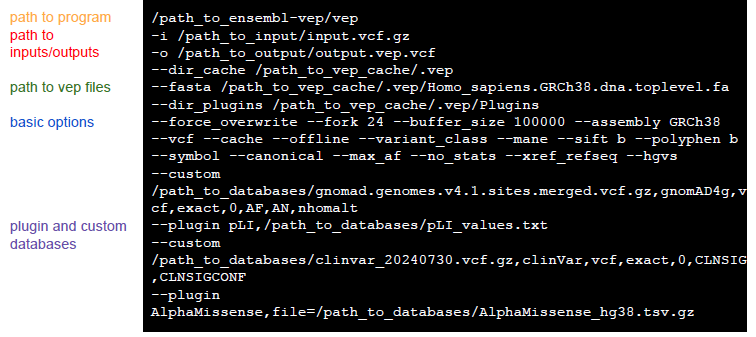
\includegraphics[width = \textwidth]{figs/ensembl-vep-commandline.png}
\caption{Ejemplo de un comando con pocas anotaciones en Ensembl. Está la ruta a la herramienta, el input y output en formato vcf comprimido o no. La caché son una serie de archivos que permite hacer las consultas en modo offline para que vaya más rápido. Los plugins están en el repositorio de GitHub y se pueden descargar para utilizarlos. Después hay una serie de opciones básicas: sobreescribir archivos en caso de existir previamente, paralelizar, número de variantes que se procesan a la vez, genoma de referencia, formato, coficiación MANE del tránscrito, que utilice Sift, PolyPhen, etc. Después se especifican los plugins y las bases de datos customizadas. En este caso, se accede a la base de datos gnomAD4g en formato VCF y se pide la anotación exacta, obteniendo la frecuencia alélica. Como se quiere utilizar la versión 4.1, se debe realizar una consulta customizada. En otros casos hay plugins existentes, como en caso de pLI, en el que no es necesario especificar qué datos debe buscar. De igual forma se especifica el plugin de AlphaMissense y se crea una consulta customizada para ClinVar.}
\end{figure}

\chapter{Priorización de variantes}
Una vez anotados los VCF, nos podemos limitar a la descripción de las variantes de un paciente o una cohorte, o realizar un análisis más detallado filtrando variantes y priorizando. Este sería el último paso, y no en todos los casos se realiza. 

\section{Visualización en IGV}
Al ver una variante interesante, se recomienda visualizarla en IGV para verificar la variante. Se pueden encontrar falsos positivos (artefactos) debido a errores de secuenciación o análisis, al igual que falsos negativos por regiones de baja cobertura o variantes de baja frecuencia. 

Cuando una variante está en los extremos de las lecturas, especialmente si está al final, puede deberse a errores en la secuenciación. Si las demás lecturas tienen esa base en el centro y no cuentan con la variante, podemos tratarlo como artefacto y falso positivo. También puede darse que una variante solo se dé en lecturas que vayan en el mismo sentido. En esos casos se trata de un sesgo y causa un falso positivo. Finalmente, si las lecturas se alinean en regiones que no están muy bien representadas en la referencia y hay muchas sustituciones, probablemente se deba a un alineamiento parálogo (las lecturas tendrían que haber alineado en otro sitio muy parecido). Estos errores no son muy frecuentes por los pasos de filtrado y refinamiento, pero pueden ocurrir. 

\section{Priorización}
La priorización se realiza utilizando un conjunto de evidencias de relevancia basadas en las anotaciones. Las anotaciones utilizadas en la priorización varían con la patología o condición en estudio. Los criterios pueden variar en función del objetivo (variantes raras, variantes comunes en la población, etc.).

Algunas evidencias para variantes clínicamente relevantes son:
\begin{itemize}
\item \textbf{Significancia clínica conocida:} ClinVar muestra si la variante es patogénica, un factor de riesgo, respuesta a fármacos.
\item \textbf{Impacto funcional:} puede ser algo o moderado en función de la consecuencia en la secuencia. Hay varios predictores del impacto funcional.
\item \textbf{Relevancia en patología:} se buscan genes implicados en procesos que están involucrados en enfermedades, o variantes frecuentes/alteraciones recurrentes de un gen o de la enfermedad
\end{itemize}

Algunas evidencias para variantes no relevantes clínicamente son variantes en tránscritos no relevantes o muy poco soportados, polimorfismos y variantes con una frecuencia poblacional mayor al 1\% salvo que esté asociado con predisposición, prognosis, respuesta a fármacos, etc.

Para el diagnóstico existen los \textbf{criterios ACMG}. Lo creó el American College of Medical Genetics and Genomics, y son normas y directrices para la interpretación de variantes de secuencia.
Se desarrollaron principalmente como un recurso educativo para los genetistas de laboratorio clínico para ayudarles a proporcionar servicios de laboratorio clínico de calidad. Las directrices del ACMG incluyen 28 criterios. Durante la interpretación de variantes, éstas se clasifican en cinco niveles: Patogénicas (P), Probablemente patogénicas (LP), Significación incierta (VUS), Probablemente benignas (LB) y Benignas (B), en función de los criterios aplicados.

\begin{figure}[htbp]
\centering
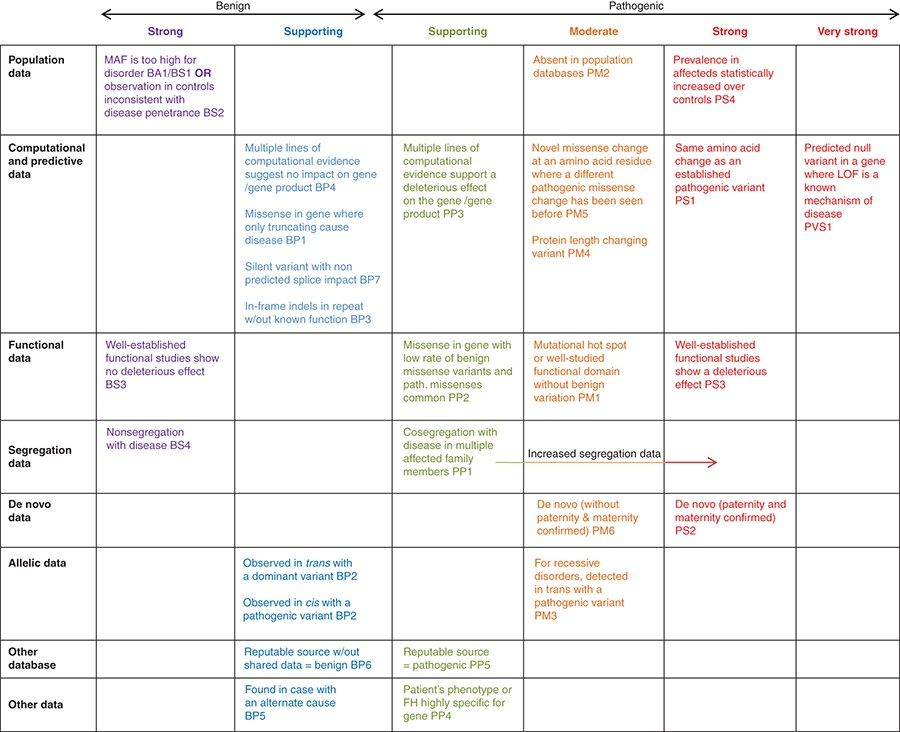
\includegraphics[width = 0.8\textwidth]{figs/acmg-guideline-table.jpg}
\end{figure}

Con la tabla anterior, se realiza un balance entre las opciones que apliquen. Cuando hay criterios de benignos y malignos, normalmente se clasifica como variante de significado incierto. 

%28/11 - Dido
\chapter{Caracterización de cohortes}
Cuando se secuencia un conjunto de muestras, se puede realizar para el diagnóstico o para hacer un análisis holístico y global (exploración de los datos). En este contexto, se pueden realizar varios pasos para ver si hay puntos en común entre los datos o si se describe alguna tendencia.

\section{Carga mutacional tumoral (TMB)}
La TMB es una medida cuantitativa del \textbf{número total de mutaciones por megabase} de ADN en el genoma de un tumor. Sirve como indicador de la \textbf{inestabilidad genómica} y a menudo se asocia con el potencial del tumor para producir neoantígenos que desencadenen una respuesta inmunitaria. El TMB se utiliza habitualmente como \textbf{biomarcador} para predecir la eficacia de la inmunoterapia, como los inhibidores de puntos de control inmunitarios, ya que un mayor TMB suele correlacionarse con mejores resultados terapéuticos. La TMB se suele calcular con mutaciones puntuales, y se pueden excluir las mutaciones sinónimas.

Hay muchas herramientas para calcular el TMB, como puede ser \href{https://github.com/anitalu724/MutScape}{MutScape}. Contiene varios sets de herramientas, como la detección de genes significativamente mutados, anotación de mutaciones asociados a cáncer o las estadísticas de la carga mutacional. Estas herramientas utilizan los ficheros en formato VCF o MAF (para esto último, se puede convertir un VCF con la herramienta \href{https://github.com/mskcc/vcf2maf}{VCF2MAF}. También calcula las mutational signatures, inestabilidad cromosómica, anotación de mutaciones accionables por fármacos, etc. 

A continuación se muestra un gráfico o plot de una cohorte de muestras tumorales divididas por el tumor primario. Se representa la carga mutacional. Testículo tiene una carga mutacional muy baja (1 mutación por megabase), pero el útero tiene mucha. Esto puede servir para poder identificar el tumor primario hipermutado. Es un buen primer enfoque para caracterizar la cohorte.

%FIXME añadir plot

\section{Oncoplot}
Un oncoplot es una representación visual utilizada habitualmente en genómica del cáncer para resumir y mostrar el panorama mutacional de una cohorte de muestras tumorales. Suele mostrar mutaciones, CNV y otras alteraciones en genes clave relacionados con el cáncer de varios pacientes, utilizando un formato similar a un mapa de calor. Cada fila representa un gen, cada columna representa una muestra y los colores o símbolos indican tipos específicos de alteraciones.

%FIXME añadir plot

Estos oncoplots se generan y trabajan con la herramienta \href{https://bioconductor.org/packages/devel/bioc/vignettes/maftools/inst/doc/maftools.html}{Maftools}. 

\href{https://www.cbioportal.org/}{Cbioportal} es una plataforma donde se han subido los genomas de muchos estudios de cáncer para poder visualizarlos a través de oncoplots. Se pueden seleccionar unos genes para buscar en muestras sacadas del atlas de cáncer pangenómico (TCGA). 

\section{Mutational signatures}
Las firmas mutacionales son \textbf{patrones únicos de mutaciones} en el ADN que reflejan los procesos subyacentes que causan alteraciones genéticas en un tumor. Estos procesos pueden incluir la exposición a factores ambientales (por ejemplo, radiación UV, fumar), deficiencias en la reparación del ADN o actividades enzimáticas. El análisis de las firmas mutacionales ayuda a identificar la etiología de las mutaciones, descubrir mecanismos de desarrollo tumoral y orientar las decisiones terapéuticas vinculando firmas específicas a posibles vulnerabilidades u opciones de tratamiento.

\href{https://cancer.sanger.ac.uk/signatures/}{COSMIC} ha generado las firmas mutacionales utilizando análisis de gran escala. Las colecciones de formas están clasificadas en función de las mutaciones que se estén analizando (mutaciones puntuales, dobletes, indels, etc). La mayoría de etiologías son desconocidas, pero sí se caracteriza una huella. La herramienta oficial es \href{https://github.com/AlexandrovLab/SigProfilerExtractor}{SigProfilerExtractor} para generar el análisis.

%FIXME añadir plot

Un patrón se puede descomponer en distintas firmas. Se puede inferir el mecanismo de acción que causó el tumor mediante el ProfilerExtractor y \href{https://github.com/AlexandrovLab/SigProfilerMatrixGenerator}{ProfilerMatrixGenerator}. 

Una vez calculadas las firmas de cada una de las muestras (aunque se computen en conjunto), se realiza la descomposición para que la composición de firmas de cada una de las muestras. Así, se puede ver si un mutor tiene la huella de haber sido tratado con quimioterapia con platino, si está asociado al tabaco, etc. 

%FIXME añadir plot de heatmap

\section{Otros aspectos relevantes}
La \textbf{inestabilidad cromosómica (CIN)} se refiere al aumento de la tasa de cambios cromosómicos, incluyendo ganancias, pérdidas y reordenamientos de cromosomas dentro de una célula. La CIN contribuye a la heterogeneidad tumoral, la progresión y la resistencia a las terapias al crear diversidad genética y promover la adaptación al estrés o a los tratamientos.

Los \textbf{neoantígenos} son péptidos de nivel que se presentan en la superficie de las células tumorales como resultado de mutaciones suáticas. Estos antígenos únicos son reconocidos por el sistema inmunitario y pueden desencadenar una respuesta inmunitaria antitumoral. Los neoantígenos son un punto clave en la inmunoterapia del cáncer, sobre todo para desarrollar vacunas personalizadas contra el cáncer e inhibidores de puntos de control inmunitario.

La \textbf{inestabilidad de microsatélites (MSI)} es una enfermedad caracterizada por la acumulación de mutaciones en secuencias repetitivas de ADN denominadas microsatélites debido a defectos en el sistema de reparación de errores de emparejamiento del ADN (MMR). La MSI suele asociarse a ciertos tipos de cáncer, como el colorrectal, el endometrial y el gástrico, y sirve como biomarcador de la respuesta a la inmunoterapia, en particular a los inhibidores de puntos de control inmunitarios.

\chapter{Copy Number Variants (CNV)}
La variación del número de copias (CNV) es un fenómeno en el que se repiten secciones del genoma
y el número de repeticiones en el genoma varía de un individuo a otro.
La variación del número de copias es un tipo de variación estructural: en concreto, es un tipo de duplicación o que afecta a un número considerable de pares de bases (genes enteros).
Aproximadamente dos tercios de todo el genoma humano pueden estar compuestos por repeticiones y el 4,8-9,5\% del genoma humano pueden clasificarse como variaciones del número de copias.
Cada vez hay más pruebas de que las CNV desempeñan un papel importante en las enfermedades humanas.

Las variaciones del número de copias se estudiaron originalmente mediante \textbf{técnicas citogenéticas}, que son técnicas que permiten observar la estructura física del cromosoma.
Una de estas técnicas es la \textbf{hibridación fluorescente in situ (FISH)}, que consiste en insertar sondas fluorescentes que requieren un alto grado de complementariedad en el genoma para unirse. Al microscopio se podían ver bandas y patrones en los cromosomas para ver si habían surgido deleciones, inserciones o translocaciones. Pequeñas CNVs no se veían.
La \textbf{hibridación genómica comparada (CGH)} también se utilizaba habitualmente para detectar variaciones en el número de copias mediante la visualización de fluoróforos y la posterior comparación de la longitud de los cromosomas, con mayor resolución. Compara la longitud esperada con la observada por fluorescencia. Con secuenciación, la detección de CNVs mejoró considerablemente. 

\section{Llamada de variantes de número de copias}
Se han desarrollado muchos algoritmos para realizar la llamada de variantes en el número de copias.
La base de estos algoritmos varía en función de la tecnología NGS utilizada para secuenciar los datos.
La secuenciación del genoma completo (WGS) a menudo utiliza estrategias de mapeo de profundidad de lectura o de extremo pareado, mientras que la secuenciación del exoma (WES) se basa en la normalización de la cobertura y el análisis de regiones específicas (si una región en lugar de tener una cobertura de 200x tiene una cobertura de 600x, se puede inferir que está triplicada; pero depende mucho de la preparación de la librería). 
Entre los principales retos a los que se enfrenta la llamada de VNC se encuentran la distinción entre variantes verdaderas y artefactos técnicos, el manejo de regiones de baja calidad y la detección fiable de puntos de rotura (breakpoints).
Una interpretación adecuada requiere algoritmos robustos y la validación con técnicas complementarias de laboratorio (como MLPA), ya que los algoritmos, sobre todo en el caso de exomas, no funcionan del todo bien.

Algunos programas para la llamada de variantes en el número de copias en \textbf{WGS} son:
\begin{itemize}
\item \href{https://github.com/Illumina/manta}{Manta}: Diseñado para detectar variantes estructurales (VS) y CNV a partir de datos WGS. Utiliza un enfoque basado en gráficos, ofreciendo una alta sensibilidad a duplicaciones, deleciones y reordenamientos complejos. Funciona bien con datos de alta cobertura y es particularmente adecuado para CNVs grandes.
\item \href{https://github.com/dellytools/delly}{Delly}: Se especializa en la detección de variantes estructurales, incluidas duplicaciones, deleciones, inserciones y translocaciones. Aprovecha las lecturas divididas y discordantes, lo que proporciona una gran precisión en conjuntos de datos WGS.
\item \href{https://genomebiology.biomedcentral.com/articles/10.1186/gb-2014-15-6-r84}{Lumpy}: Un llamador de variantes estructurales que combina lecturas divididas, lecturas discordantes y profundidad de cobertura. Eficaz para datos WGS, capaz de detectar CNV de varios tamaños y tipos.
\end{itemize}

Para \textbf{WGS}, se utilizan:
\begin{itemize}
\item \href{https://cnvkit.readthedocs.io/en/stable/}{CNVkit}: Diseñado específicamente para datos WES, pero también compatible con paneles específicos. Normaliza la profundidad de lectura a la vez que tiene en cuenta las características únicas de los diseños de captura de exomas. Alta precisión para CNV pequeñas y medianas en regiones codificantes.
\item \href{https://github.com/vplagnol/ExomeDepth}{ExomeDepth}: Paquete R adaptado para WES, que compara la profundidad de lectura entre muestras con un panel de controles. Muy adecuado para aplicaciones clínicas, ya que ofrece una alta sensibilidad y especificidad en las regiones capturadas.
\item \href{https://www.nature.com/articles/s41588-023-01449-0}{GATK gCNV}: Parte de la suite GATK, desarrollada para la detección de CNV en WES. Utiliza un modelo bayesiano para integrar datos de múltiples muestras y mejorar la precisión.
\end{itemize}

Una base de datos que recoge la frecuencia poblacional de CNVs es \href{https://dgv.tcag.ca/dgv/app/about}{DGV o Database of Genomic Variants}. Resumen de la variación estructural en el genoma humano (alteraciones genómicas que afectan a segmentos de ADN de más de 50 pb). El contenido de la base de datos sólo representa la variación estructural identificada en muestras de control sanas, por lo que proporciona un catálogo útil de datos de control para los estudios que pretenden correlacionar la variación genómica con los datos fenotípicos. La base de datos se actualiza continuamente con nuevos datos procedentes de estudios de investigación revisados por expertos.

\chapter{Snakemake y pipeline management}
Todos los pasos vistos anteriormente se deben automatizar, ya que es inviable realizar los pasos individuales para una gran cantidad de muestras.

Snakemake es un potente y flexible sistema de gestión de flujos de trabajo diseñado para crear pipelines de análisis de datos reproducibles y escalables utilizando un lenguaje basado en Python.
Utiliza una sintaxis declarativa para definir flujos de trabajo, donde cada paso (o «regla») especifica la entrada, la salida y los comandos para procesar los datos.
Snakemake determina automáticamente las dependencias entre los pasos y los ejecuta de manera eficiente, ya sea en una máquina local, un clúster o un entorno en la nube.

Para un proceso de análisis de variantes somáticas y de línea germinal, Snakemake proporciona la estructura para integrar múltiples herramientas y scripts en un flujo de trabajo cohesivo.
Garantiza un orden de ejecución adecuado, gestiona archivos intermedios y admite puntos de comprobación y pasos condicionales para canalizaciones dinámicas.

Los ficheros necesarios para un workflow en Snakemake son:
\begin{itemize}
\item \textbf{Snakefile:} es el archivo central que define el flujo de trabajo. Contiene reglas que especifican cómo se transforman los archivos de entrada en archivos de salida, comandos para herramientas de llamada de variantes (BWA, GATK, MuTect2, etc) y dependencias entre pasos (por ejemplo, alineación $\rightarrow$ llamada de variantes $\rightarrow$ anotación).

\begin{figure}[h!]
\centering
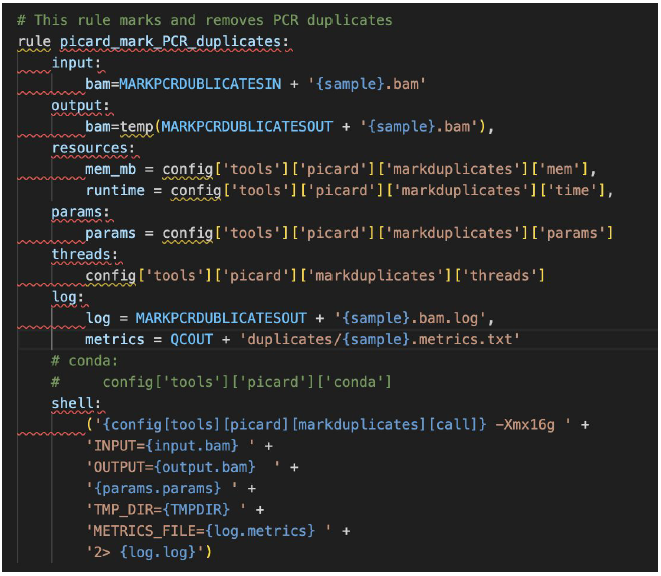
\includegraphics[width = 0.36\textwidth]{figs/snakemake-rule.png}
\end{figure}

\item \textbf{Fichero de configuración (config.yaml):} almacena parámetros personalizables para la pipeline, tales como rutas de archivos para los datos de entrada (FastQ, BAM, etc) y rutas del genoma de referencia, ajustes específicos de la herramienta (por ejemplo, umbrales de mutación o ploidía). Permite la reutilización y simplifica la adaptación del proceso a nuevos conjuntos de datos.

\begin{figure}[htbp]
\centering
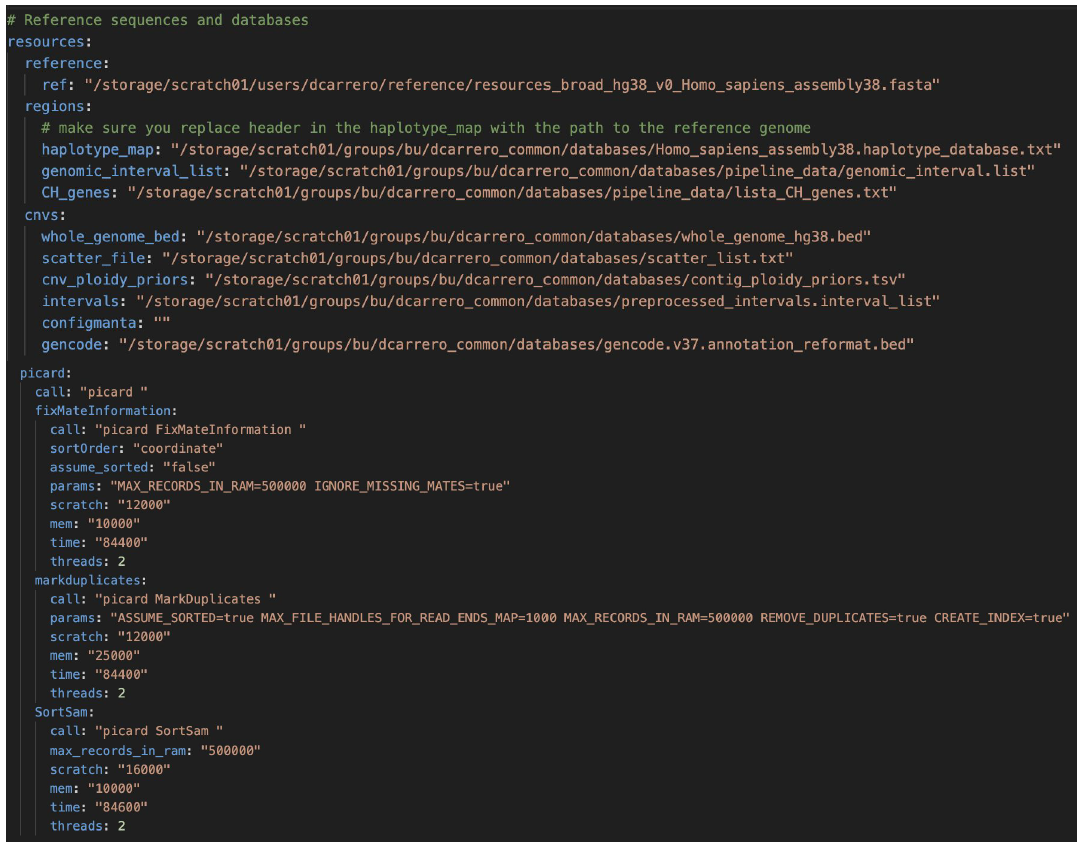
\includegraphics[width = 0.5\textwidth]{figs/snakemake-config.png}
\end{figure}

\item \textbf{Entornos o módulos:} garantizan un entorno de software coherente y reproducible. Cuenta de archivos de entorno conda (environment.yaml) o definiciones de módulos para herramientas y dependencias necesarias. 

\begin{figure}[htbp]
\centering
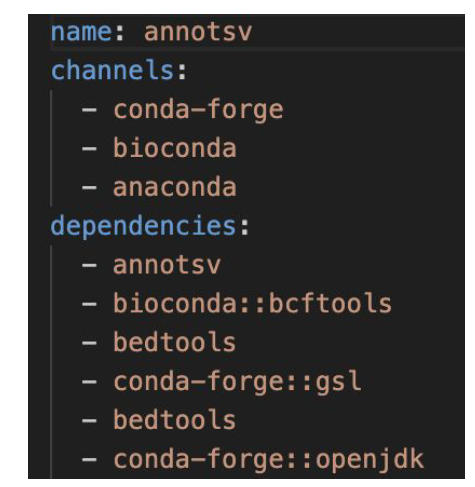
\includegraphics[width = 0.3\textwidth]{figs/snakemake-env.png}
\end{figure}
\end{itemize}

Snakemake permite crear un gráfico con todos los pasos de la pipeline para verificar si los pasos están ordenados de forma correcta.
%29/11 - Lucía Sánchez
\part{Genome/Phenome Analysis}
\chapter{Genome-Wide Association Studies (GWAS)}
\section{Introducción a GWAS y características}
Los \textbf{estudios de asociación a nivel del genoma} (GWAS, por sus siglas en inglés) son un enfoque utilizado para identificar variantes genéticas asociadas a rasgos o enfermedades específicas en una población. Estos estudios analizan la asociación entre \textbf{variantes genéticas comunes} y fenotipos mediante el genotipado de grandes cantidades de SNPs (Single-Nucleotide Polymorphisms) en múltiples individuos.

El gráfico ilustra la relación entre \textbf{frecuencia alélica} y \textbf{penetrancia}. La penetrancia mide el porcentaje de individuos portadores de una variante genética que desarrollan un fenotipo o enfermedad. Por otro lado, la frecuencia alélica indica la proporción en la población de un alelo determinado que causa un fenotipo.
\begin{itemize}
\item \textbf{Enfermedades mendelianas:} tienen alta penetrancia (con una mutación se desarrolla la enfermedad) pero baja frecuencia alélica. Un ejemplo es la talasemia, una enfermedad autosómica recesiva que afecta la síntesis de las cadenas alfa y beta de la hemoglobina, provocando anemia severa.
\item \textbf{Enfermedades complejas:} tienen baja penetrancia pero alta frecuencia alélica. GWAS se enfoca en estas variantes comunes que influyen parcialmente en el riesgo de enfermedades complejas como las enfermedades cardiovasculares, que involucran factores genéticos y ambientales.
\end{itemize}

\begin{figure}[htbp]
\centering
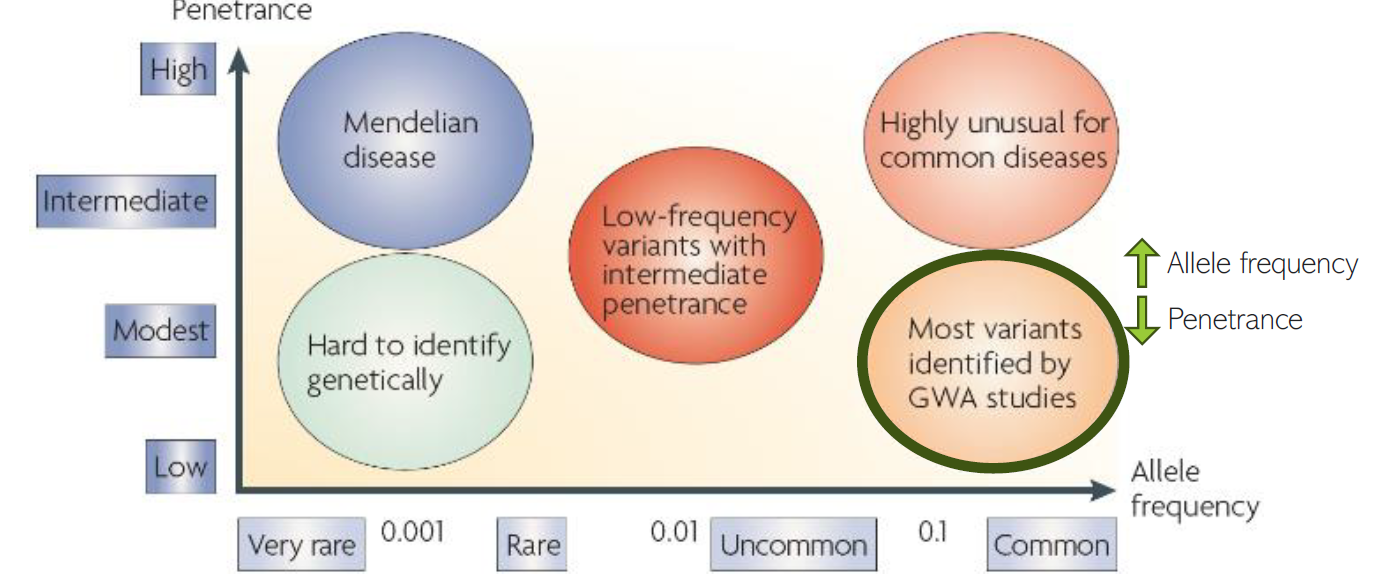
\includegraphics[width = \textwidth]{figs/gwas.png}
\end{figure}

Las variantes estudiadas en GWAS son:
\begin{itemize}
\item Single-Nucleotide Variant (SNV): Cambios de una sola base en el ADN causados por errores durante la meiosis o daño en el ADN de las células germinales.
\item Single-Nucleotide Polymorphism (SNP): SNVs presentes en al menos un 1\% de la población.
\end{itemize}

GWAS analiza grandes cantidades de SNPs (entre 500,000 y 1,000,000 por muestra). Esto es posible gracias a plataformas tecnológicas como Illumina y Affymetrix.

Las herramientas utilizadas en GWAS son:
\begin{itemize}
\item PLINK: Software especializado en la manipulación, resumen y limpieza de datos genéticos.
\item R: Utilizado para análisis estadístico y visualización.
\item Bases de datos:
\begin{itemize}
\item dbSNP: Para obtener información sobre variantes conocidas.
\item GWAS Catalog: Repositorio de estudios GWAS publicados.
\end{itemize}
\end{itemize}

\section{Realizar un GWAS}
El primer paso es \textbf{seleccionar una población de estudio}. Esto depende de la pregunta experimental y hay que tener un tamaño muestral suficiente para asegurar potencia estadística. Si el estudio es dicotómico, habría que tener casos y controles para ver la asociación entre presencia y ausencia. Si por el contrario el estudio es cuantitativo, hay que tener medidas cuantitativas. 

A las personas se las \textbf{genotipa} mediante Whole-genome Sequencing (WGS), whole-exome sequencing (WES) o microarrays (análisis de SNPs concretos para analizar variantes preseleccionadas). 

Una vez secuenciados los datos, hay que \textbf{procesarlos}. En algunos casos hay que anonimizar los datos, ver si hay relaciones familiares entre muestras, sexo, información fenotípica, etc. También es necesario realizar control de calidad. La imputación permite predecir variantes no genotipadas mediante patrones de asociación conocidos. Por último, se realiza un \textbf{test de asociación} para analizar la relación entre variantes genéticas y el fenotipo.

\subsection{Control de calidad}
\subsubsection{Missingness}
En el control de calidad, se mira el missingness o la ausencia tanto por SNP como por individuo. Se eliminan los SNPs o individuos con altos porcentajes de datos ausentes. Los valores recomendados son tener al menos un 95\% de información por muestra y un 95-99\% de información por SNP (call rate).

\begin{figure}[htbp]
\centering
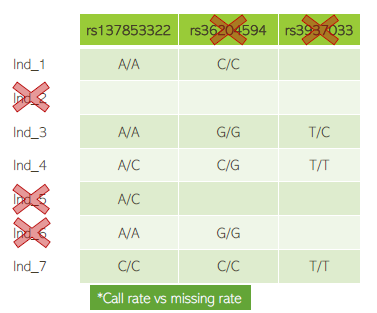
\includegraphics[width = 0.8\textwidth]{figs/missingness.png}
\end{figure}

\subsubsection{Discrepancia por sexo}
Se verifica la concordancia entre el sexo genotípico (tasa de homocigosis en el cromosoma X) y el sexo declarado.

%Para estudiar la discrepancia por sexo, se mira la diferencia entre el sexo asignado y el determinado basado en la información genotípica. Se determina mediante la computación de la tasa de homocigosis de los SNP del cromosoma X.

\subsubsection{Minor Allele Frequency (MAF)}
El Minor Allele Frequency (MAF) se define como la frecuencia del alelo menos frecuente en cada locus. Los GWAS se centran en variantes comunes asociadas a enfermedades en la población. Las variantes raras tienen baja potencia estadística.
Las variantes con un MAF muy bajo también se ven afectadas más fácilmente por errores de genotipado. Se utilizan los siguientes límites: 1-5\% para GWAS de unos cientos o mil individuos y más bajo (0,1\%) para tamaños muestrales más grandes, como UK Biobank.

\subsubsection{Hardy-Weinberg Equilibrium (HWE)}
El equilibrio de Hardy-Weinberg o ley de Hardy-Weinberg establece que en un apareamiento aleatorio tanto las frecuencias alélicas como genotípicas de una población permanecen invariables. Para que este equilibrio se dé, se deben cumplir los siguientes supuestos: apareamiento aleatorio, alelos femeninos y masculinos independientes, frecuencias alélicas idénticas entre machos y hembras, tamaño poblacional grande (infinito), no hay efecto de migración, mutación o selección natural. Para calcular las frecuencias genotípicas, se utiliza la siguiente fórmula:
$$P(G_i) = \sum_{j=1}^6 P(G_i|MT_j) \cdot P(MT_j)$$

\begin{figure}[htbp]
\centering
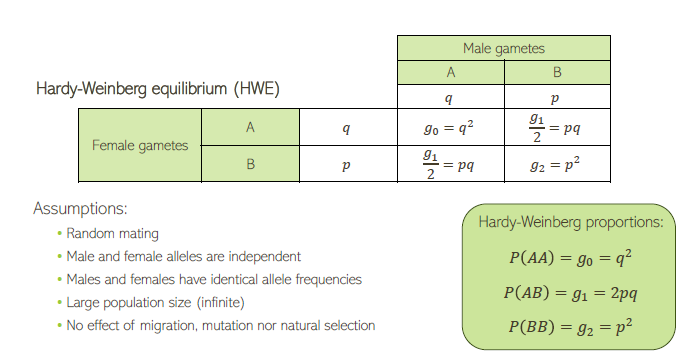
\includegraphics[width = \textwidth]{figs/hwe.png}
\end{figure}

Para asimilar esto, vamos a realizar un ejercicio en el que calculamos el equilibrio Hardy-Weinberg:
\begin{table}[h!]
\centering
\begin{tabular}{|l|c|ccc|}
\hline
\textbf{Mating types} & \textbf{Frequency} & \multicolumn{3}{c|}{\textbf{Frequency of zygotes}} \\ 
\cline{3-5}
                      &                    & \textbf{AA} & \textbf{AB} & \textbf{BB} \\ \hline
MT1: AA x AA          & $g_0g_0 = g_0^2$   & 1           & -           & -           \\
MT2: AA x AB          & $g_0g_1+g_1g_0 = 2g_0g_1$ & 0.5         & 0.5         & -           \\
MT3: AA x BB          & $g_0g_2 + g_2g_0= 2g_0g_2$ & -           & 1           & -           \\
MT4: AB x AB          & $g_1g_1 = g_1^2$   & 0.25        & 0.5         & 0.25        \\
MT5: AB x BB          & $g_1g_2+g_2g_1 = 2g_1g_2$ & -           & 0.5         & 0.5         \\
MT6: BB x BB          & $g_2g_2 = g_2^2$   & -           & -           & 1           \\ \hline
\end{tabular}
\caption{Tabla de frecuencias de tipos de apareamiento y cigotos.}
\label{tab:zygotes}
\end{table}

En base a los resultados de la tabla \ref{tab:zygotes}, las frecuencias genotípicas son:
$$q^2 = P(AA) = 1 \cdot g_0^2 + \frac{2g_0g_1}{2} + \frac{g_1^2}{4} = g_0^2 + g_0g_1 + \frac{g_1^2}{4} = (g_0 + \frac{g_1}{2})^2$$
$$p^2 = P(BB) = \frac{g_1^2}{4} + \frac{2g_1g_2}{2} + g_2^2 = \frac{g_1^2}{4} + g_1g_2 + g_2^2 = (g_2 + \frac{g_1}{2})^2$$
$$2pq = P(AB) = \frac{2g_0g_1}{2} + 1 \cdot 2g_0g_2 + \frac{g_1^2}{2} + \frac{2g_1g_2}{2} = g_0g_1 + 2g_0g_2 + \frac{g_1^2}{2} + g_1g_2 = 2(g_2 + \frac{g_1}{2})(g_0 + \frac{g_1}{2})$$

Para testar las proporciones HWE, se utiliza el test del chi cuadrado.

\begin{figure}[htbp]
\centering
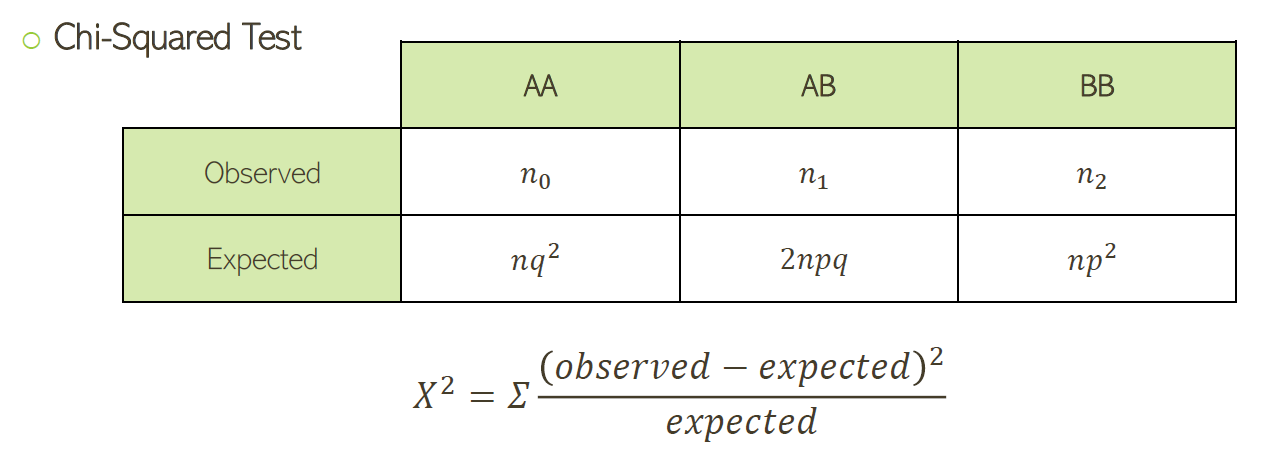
\includegraphics[width = \textwidth]{figs/chi-cuadrado.png}
\end{figure}

Mide lo que difiere los resultados observados con los resultados esperados. El problema es que con los GWAS, este test no es del todo preciso, por lo que se emplea el exact test.

Una vez calculado el HWE y con el test se ve cómo difieren los resultados, se ve si se está violando la ley de HW, es decir, si las frecuencias genotípicas son significativamente diferentes de las esperadas. En GWAS, se asume que desviaciones de HWE se deben a errores del genotipado. En el caso de estudios binarios, el límite del HWE es menos estricto en casos que en controles, ya que la violación de la ley puede indicar una asociación genética real con riesgo a enfermedad. Para estudios cuantitativos, se emplea un p-valor menor a 1e-6. 

\subsubsection{Heterocigosidad}
La heterocigosidad indica la proporción de loci heterocigotos en un individuo, es decir, se refiere a la presencia de los dos alelos en un SNP de un individuo. Se recomienda eliminar todos los individuos que se desvíen $\pm 3 SD$ de la media:
$$HeterozygosityRate_ind = \frac{NonMissingCounts - HomozygousGenotypeCount}{NonMissingCounts}$$
Un alto nivel de heterozigosidad se puede deber a una calidad baja de las muestras o contaminación, y unos niveles bajos a inbreeding o una relación entre las muestras.

\subsubsection{Relatedness}
Relatedness es el último paso del control de calidad. En los GWAS más comunes, se asume que no hay asociación entre los participantes del estudio. El grado de relatedness se puede definir como número de alelos compartidos entre los individuos dos a dos. Se mide mediante identity by descent (IBD), que es la proporción de los genomas de dos individuos compartiendo alelos heredados de un ancestro común. 

\begin{figure}[htbp]
\centering
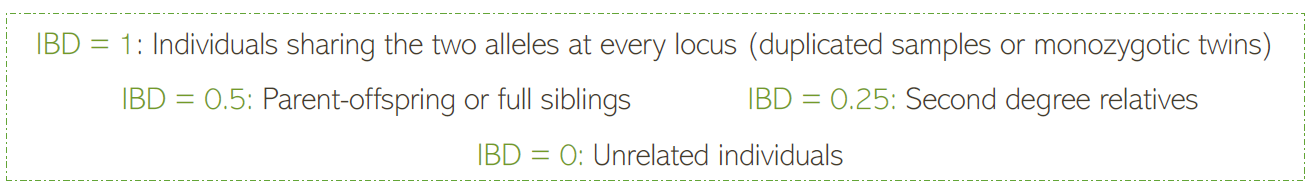
\includegraphics[width = \textwidth]{figs/ibd.png}
\end{figure}

Se diferencian Identity-by-state (IBS) de Identity-by-descent (IBD). En IBS, los alelos compartidos entre individuos son en un locus particular debido a evolución convergente, ancestros comunes o eventos mutacionales similares y se computa como sin información sobre herencia, mientras que en IBD los alelos compartidos entre individuos en un locus particular se debe a un ancestro comun y se debe estimar la probabilidad de heredad la misma copia de un alelo.

En estudios de población estándar, se recomienda eliminar uno de los individuos con un IBD mayor de 0,2. El desequilibrio de ligamiento hace referencia a la herencia conjunta de genes en diferentes loci en el mismo cromosoma en una población concreta. Los SNP están en LD cuando la frecuencia de asociación de sus alelos es superior a la esperada si los loci fueran independientes y estuvieran asociados al azar. 

\section{Práctica: Proyecto HapMap internacional}
El objetivo es elaborar un mapa de haplotipos del genoma humano. La información está disponible gratuitamente en conjuntos de datos públicos. Comenzó con una reunión, celebrada del 27 al 29 de octubre de 2002, y alcanzó su objetivo de completar el mapa en tres años. Se trata de una colaboración entre investigadores de centros académicos, grupos de investigación biomédica sin ánimo de lucro y empresas privadas de Japón, Reino Unido, Canadá, China, Nigeria y Estados Unidos. El HapMap identifica entre 250.000 y 500.000 SNP marcados (casi tanta información cartográfica como los 10 millones de SNP). Cuenta con muestras procedentes de Yoruba, Japón, China y Estados Unidos (residentes en Utah con ascendencia del norte y oeste de Europa).

Los haplotipos son un conjunto de alelos de un cromosomas que se han heredado conjuntamente de un mismo progenitor al estar localizados de forma próxima en el cromosoma. Se puede limitar a un solo gen o a múltiples. Los \textbf{TagSNP} son SNPs representativos en una región del genoma con un alto linkage disequilibrium. 

\begin{figure}[htbp]
\centering
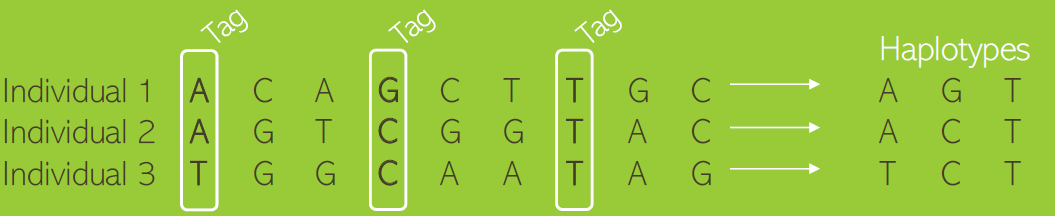
\includegraphics[width = \textwidth]{figs/tagsnp.png}
\end{figure}

El Proyecto Internacional HapMap nació para desarrollar un mapa de haplotipos del genoma humano. 

Durante las prácticas de esta parte de la asignatura, haremos uso de los datos del HapMap para determinar asociaciones entre los SNPs de este estudio y la variable de resultado, en lo que se conoce como estudios de asociación de genoma completo (GWAS).

Como ya hemos visto en clase, el control de calidad es el primer paso en los GWAS. Este proceso es crucial para eliminar las muestras de baja calidad, la contaminación, deshacerse de los errores generados durante el SNP calling o controlar la subestructura de la población, entre otras cosas. Esto es esencial para asegurar que nuestros datos tienen suficiente calidad para realizar las pruebas de asociación.

Como recordatorio, el control de calidad se divide en algunos pasos:
\begin{enumerate}
\item Control for missingness
\item Sex Discrepancy
\item Minor allele frequency
\item Hardy-Weinberg equilibrium
\item Heterozygosity
\item Relatedness
\item Population substructure
\end{enumerate}

En este pipeline, controlaremos los seis primeros pasos. Para ello se utilizará principalmente PLINK, una herramienta que permite estudiar las características de los datos y limpiarlos de forma sencilla y eficaz. También se utilizará R para trazar algunos resultados y ayudar en la determinación de los umbrales (librerías ggplot2 y dplyr).

\subsection{Missingness por individuo y por SNP}
La falta de datos (missingness) se refiere al grado de datos no disponibles a nivel de SNP o de individuo y está directamente asociada con la calidad de los datos. Una buena práctica consiste en eliminar los SNP/individuos con una elevada proporción de omisión.

Para determinar esta proporción, podemos utilizar `--missing` de PLINK. Este flag genera dos archivos que muestran la proporción de SNPs perdidos por individuo y la proporción de individuos perdidos por SNP, respectivamente. 

En este paso, se crean los ficheros plink.lmiss con la información de missigness de los SNP y plink.imiss con la información de missigness de los individuos.

\begin{lstlisting}[language=bash]
plink --bfile HapMap_3_r3_1 --missing --out plink
\end{lstlisting}

Como dice el informe, tenemos 1457897 variantes y 165 personas (80 hombres / 85 mujeres).

\subsection{Estudio de Missingness de SNP}

\begin{lstlisting}[language=R]
snpmiss <- read.table(file="plink.lmiss", header=TRUE)

kable(head(snpmiss), caption = "SNP missingness information") %>%
  kable_styling(bootstrap_options = c("striped", "hover", "condensed", "responsive"), full_width = FALSE) 
\end{lstlisting}

Una vez cargados los datos, los visualizamos:

\begin{lstlisting}[language=R]
p <- ggplot(snpmiss, aes(x=F_MISS)) +
  geom_histogram(color="black", fill="#E69F00", binwidth=.0025) +
  ggtitle('Histogram SNP missingness') +
  ylab('Frequency') +
  geom_vline(xintercept = .02, linetype="dotted",
               color = "black", linewidth=.9)
p 
\end{lstlisting}

\begin{figure}[htbp]
\centering
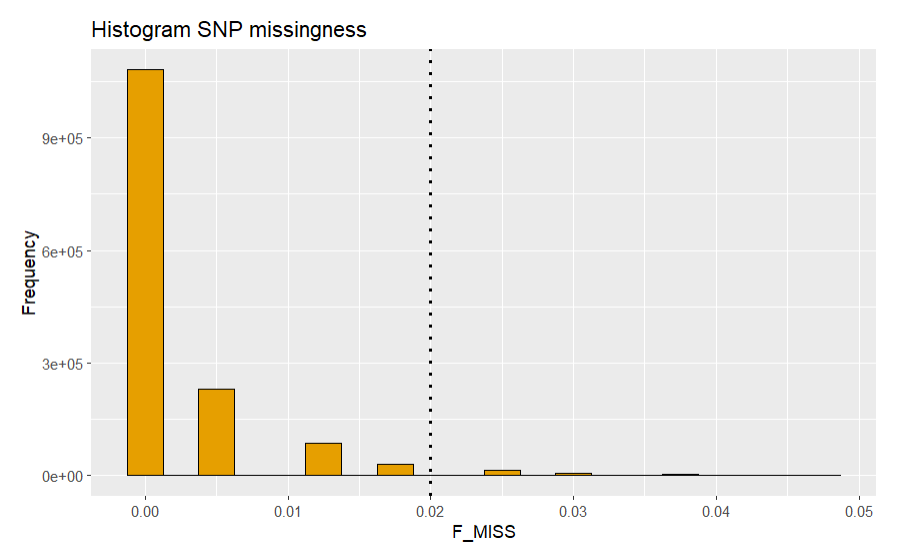
\includegraphics[width = 0.8\textwidth]{figs/hist-snpmiss.png}
\end{figure}

Imaginemos que decidimos fijar un umbral en 0,02. Esto significa que estamos eliminando SNPs con más del 2\% de su información faltante.
\begin{lstlisting}[language=R]
sum(snpmiss$F_MISS > 0.02)
\end{lstlisting}

En total estamos eliminando 27454 valores. Para ver la cantidad de individuos que deben tener una ausencia información para ese SNP para que se elimine, se realiza el siguiente código y el resultado son 4 personas.
\begin{lstlisting}[language=R]
deleted_snp <- snpmiss[snpmiss$F_MISS > 0.02, ]
min(deleted_snp$N_MISS)
\end{lstlisting}

\subsubsection{Estudio de missingness de individuos}
De forma similar a como hemos hecho con el SNP missingness, queremos detectar el missingness individual. Para ello, cargar el archivo que contiene esta información y, representar los individuos falta en un histograma:
\begin{lstlisting}[language=R]
indmiss <- read.table("plink.imiss", header = TRUE)

p <- ggplot(indmiss, aes(F_MISS)) +
  geom_histogram(color="black", fill="#E69F00", binwidth=.0005)

p
\end{lstlisting}

\begin{figure}[htbp]
\centering
\includegraphics[width = 0.8\textwidth]{figs/hist-indmiss.png}
\end{figure}

Decidimos fijar de nuevo el umbral en 0,02. Esto significa que se eliminan los individuos con más de un 2\% de omisión en sus SNP, que en este caso es una persona.
\begin{lstlisting}[language=R]
sum(indmiss$F_MISS > 0.02)
\end{lstlisting}

Para ver la cantidad de SNPs que deben estar ausentes en un individuo para eliminarlo, se realiza el siguiente cálculo y el resultado son 29584.
\begin{lstlisting}[language=R]
deleted_ind <- indmiss[indmiss$F_MISS > 0.02, ]
min(deleted_ind$N_MISS)
\end{lstlisting}

\subsubsection{Filtrar SNPs e individuos}
Después de representar los resultados, concluimos que el 2\% de missingness es un buen umbral tanto para SNPs como para individuos. Por lo tanto, debemos utilizar `--geno` y `--mind` para eliminar ese porcentaje.

\begin{lstlisting}[language=bash]
# Delete SNPs with missingness >0.02.
plink --bfile HapMap_3_r3_1 --geno 0.02 --make-bed --out HapMap_3_r3_2

# Delete individuals with missingness >0.02.
plink --bfile HapMap_3_r3_2 --mind 0.02 --make-bed --out HapMap_3_r3_3
\end{lstlisting}

Tras analizar el output, vemos que no se ha eliminado ningún individuo. Esto se debe a que, como primero se eliminan los SNP, se recalcula el missingness para los individuos y el que antes sí eliminábamos, ya no cumple con la condición (los SNPs de los que no tenía información son aquellos que se han eliminado por tener poca información de individuos).

%02/12 - Lucía Sánchez
A continuación miramos la discrepancia entre sexos. La discrepancia de sexo se refiere a la diferencia entre el sexo asignado y el determinado. Puede estudiarse con `--check-sex`, que genera un documento con 6 columnas:
\begin{enumerate}
\item FID: family ID
\item IID: individual ID
\item PEDSEX: sex from the pedigree file (1 = male, 2 = female)
\item SNPSEX: sex determined by X chromosome
\item STATUS: problem/ok
\item F: the actual X chromosome inbreeding (homozygosity) estimate. This estimate allows to determine the sex of the individuals, being F < 0.2 assigned to females, and F > 0.8, to males.
\end{enumerate}

Primero utilizamos ese flag para determinar el número de personas con sexo masculino y femenino:
\begin{lstlisting}[language=bash]
plink --bfile HapMap_3_r3_3 --check-sex --out plink
\end{lstlisting}

Ese fichero se carga en R y se genera un histograma con F estimado:
\begin{lstlisting}[language=R]
sex <- read.table("plink.sexcheck", header = TRUE)
p <- ggplot(sex, aes(F)) +
  geom_histogram(color="black", fill="#E69F00", binwidth=.005)
p
\end{lstlisting}

Para ver el número de hombres y mujeres predichos:
\begin{lstlisting}[language=R]
#males
sum(sex$SNPSEX == 1)

#females
sum(sex$SNPSEX == 2)
\end{lstlisting}
Obtenemos 81 hombres y 84 mujeres. Ahora queremos ver si hay alguna discordancia entre el sexo predicho y el computado:
\begin{lstlisting}[language=R]
discordance <- sex[sex$PEDSEX != sex$SNPSEX,]
discordance
\end{lstlisting}

Vemos que hay un individuo que discrepa, por lo que queremos filtrarlo. Generamos un fichero .txt con el FID e IID de la persona problemática.
\begin{lstlisting}[language=bash]
grep "PROBLEM" plink.sexcheck | awk '{print $1, $2}' > sex_discrepancy.txt
\end{lstlisting}

Posteriormente utilizamos el flag --remove para eliminar los individuos en el fichero txt.
\begin{lstlisting}[language=bash]
plink --bfile HapMap_3_r3_3 --remove sex_discrepancy.txt --make-bed --out HapMap_3_r3_4
\end{lstlisting}

Ahora analizamos minor allele frequency (MAF). El MAF se refiere a la frecuencia del alelo menos frecuente en un locus. Debemos eliminar los SNP con un MAF bajo porque la potencia estadística de los GWAS no permite detectar asociaciones si la frecuencia del alelo es demasiado baja. Generamos un fichero .txt con los SNPs autosomales y después eliminamos aquellos con el MAF más pequeño. 
\begin{lstlisting}[language=bash]
# Select autosomal SNPs (from chromosomes 1 to 22).
awk '{ if ($1 >= 1 && $1 < 23) print $2}' HapMap_3_r3_4.bim > snp_1_22.txt
#Remove unlisted variants
plink --bfile HapMap_3_r3_4 --extract snp_1_22.txt --make-bed --out HapMap_3_r3_5
\end{lstlisting}

A continuación utilizamos el flag --freq para computar el MAF en los cromosomas autosomales.
\begin{lstlisting}[language=bash]
plink --bfile HapMap_3_r3_5 --freq --out plink
\end{lstlisting}

Cargamos el fichero generado y representamos la distribución de MAF en un histograma, estableciendo un límite del 5\%.
\begin{lstlisting}[language=R]
maf_freq <- read.table("plink.frq", header = TRUE)
p <- ggplot(maf_freq, aes(MAF)) +
	geom_histogram(color="black", fill="#E69F00", binwidth=.005) +
	geom_vline(xintercept = .05, linetype="dotted", color = "black", linewidth=.9)
p
\end{lstlisting}

Estamos eliminando 1073226 SNPs y quedándonos con 325318.
\begin{lstlisting}[language=R]
#deleting
sum(maf_freq$MAF >= 0.05)
#retaining
sum(maf_freq$MAF < 0.05)
\end{lstlisting}

Eliminamos los SNPs.
\begin{lstlisting}[language=bash]
plink --bfile HapMap_3_r3_5 --maf 0.05 --make-bed --out HapMap_3_r3_6
\end{lstlisting}

El siguiente paso es eliminar los SNPs que no estén en equilibrio Hardy-Weinberg. El equilibrio de Hardy-Weinberg (HWE) establece que, en un apareamiento aleatorio, las frecuencias alélicas y genotípicas permanecen constantes o estables en una población si no se introducen factores perturbadores. `--hardy` escribe una lista de recuentos de genotipos y estadísticas de la prueba exacta de equilibrio Hardy-Weinberg.
\begin{lstlisting}[language=bash]
plink --bfile HapMap_3_r3_6 --hardy --out plink
\end{lstlisting}

Posteriormente elegimos los SNPs con un p-valor HWE < 0,0001.
\begin{lstlisting}[language=bash]
awk '{ if ($9 <0.00001) print $0 }' plink.hwe > plinkzoomhwe.hwe
\end{lstlisting}

Y ahora creamos los histogramas:
\begin{lstlisting}[language=R]
hwe <- read.table("plink.hwe", header = TRUE)
hwe
p <- ggplot(hwe, aes(P)) +
  geom_histogram(color="black", fill="#E69F00", binwidth=.05)
p

hwe_zoom <- read.table("plinkzoomhwe.hwe", header = FALSE)
hwe_zoom
p <- ggplot(hwe_zoom, aes(V9)) +
  geom_histogram(color="black", fill="#E69F00")
p
\end{lstlisting}

\section{Consideraciones de GWAS}
En cuanto al diseño del estudio, pueden diferenciarse los estudios basados en población, en familia o en poblaciones aisladas.

\subsection{Population-based GWAS}
Se trata de un estudio de asociación genética con individuos no emparentados. El estudio más común es uno de casos y controles, siendo los casos personas con presencia de un fenotipo y los controles ausencia del mismo. Los individuos pueden seleccionarse activamente y los controles se pueden emparejar con los casos (con respecto al sexo, factores de riesgo, ...). Se realiza un reclutamiento activo. Estos estudios tienen buena potencia y son rentables si la frecuencia de la enfermedad en la población es baja (<20\%). Si la frecuencia de los casos es mayor que la frecuencia basada en población, se debe ajustar por covariantes durante el análisis estadístico. Los casos y controles que no se genotipen conjuntamente deben tener una corrección (batch correction) para ajustar por covariables.

Los estudios de casos y controles se pueden clasificar en estudios retrospectivos y prospectivos. En los \textbf{estudios retrospectivos}, los sujetos se seleccionan en función de su estado de enfermedad. Se suele utilizar con enfermedades raras, ya que no es viable escoger participantes y esperar a que generen la enfermedad. Se obtienen los datos genéticos y ambientales.

En los \textbf{estudios prospectivos}, se establece una cohorte y se realiza un genotipado base de todos los sujetos. Se realiza un seguimiento de los individuos y se observa si hay un desarrollo de la enfermedad. Aquellos que la desarrollen pasan a ser controles, y aquellos que no serán los controles. 

Las ventajas es que estos estudios son muy rentable para asociaciones a gran escala, pero tiene la desventaja de obtener subgrupos poblacionales, generando asociaciones falsas debido a las subpoblaciones.

\subsection{Family-based GWAS}
Este estudio utiliza sujetos recogidos en familias, y se utilizó frecuentemente en los inicios de GWAS. En el caso del trío caso-padres, se genotipa a la descendencia afectada y a los padres. Se compara entre el número de alelos marcadores transmitidos de padres a descendientes con el número de alelos no transmitidos. Se puede tralizar la prueba de desequilibrio de transmisión (TDT) o prueba de asociación para identificar el vínculo genético entre un marcador genético (SNP) y un rasgo (fenotipo). Examina la segregación de un alelo dentro de una familia. La ventaja es que es robusto frente a estratificación poblacional y con enfermedades de baja prevalencia (< 1\%). Además, se estudian los efectos de un alelo en un fenotipo individual de sus efectos indirectos en miembros familiares cercanos. No obstante, se requiere un tamaño muestral más grande que el GWAS poblacional para alcanzar la misma potencia estadística y es menos eficiente en el caso de enfermedades de aparición tardía.

\subsection{Poblaciones aisladas}
Las poblaciones aisladas son grupos separado de sus poblaciones vecinas por barreras (geográficas, culturales o lingüísticas) y que tienen un flujo genético mínimo desde ellas. Estas poblaciones aisladas han permanecido aisladas durante un periodo prolongado, teniendo un flujo genético restringido con las poblaciones vecinas. Estos estudios tienen una mayor precisión de imputación que otras pruebas con un desequilibrio de ligamiento de largo alcance. 
Los descubrimientos en poblaciones aisladas son muy difíciles de replicar en otras poblaciones. Así, variantes funcionales raras pueden estar presente en mayor frecuencia en poblaciones aisladas, habiendo así una potencia aumentada para estudios de asociación de estas variantes.

\subsection{Subestructura poblacional - práctica}
En esta práctica estudiaremos relatedness y la estratificación poblacional. La estratificación poblacional puede ser la principal fuente de confusión. Ejemplo: estudio de casos y controles, en el que las diferencias genotípicas entre casos y controles se deben a los distintos orígenes de la población (casos: europeos, controles: asiáticos) y no a un efecto sobre el riesgo de enfermedad. La confusión se debe a que la subestructura de la población no está distribuida por igual entre los grupos de casos y controles. Así, una señal de asociación surgirá no por una asociación entre un fenotipo y un SNP, sino por diferencias de frecuencia alélica entre las poblaciones que comprenden los casos y los controles. Esto tiene dos soluciones: eliminar los individuos de ascendencia divergente o establecer la ascendencia como covariable/efecto aleatorio en modelos mixtos.

Los métodos para identificación de individuos con diferencias a larga escala en ascendencia es mediante una PCA (principal component analysis) o MDS (multidimensional scaling). MDS calcula la proporción de alelos compartidos entre cada par de individuos para identificar la variación genética para cada individuo. Los resultados se muestran en un gráfico para explorar la distribución de individuos en los datos. Por ejemplo, estudio genético que incluya sujetos de Asia y Europa. El análisis MDS revelaría que los asiáticos son genéticamente más parecidos entre sí que a los europeos.

\end{document}
